%%%%%%%%%%%%%%%%%%%%%%%%%%%%%%%%%%%%%%%%%
% Design based on a template by Roberto and following the format of
% the xmipp tutorials. In turn, they seem to be based on a template
% from http://www.latextemplates.com
%%%%%%%%%%%%%%%%%%%%%%%%%%%%%%%%%%%%%%%%%

%----------------------------------------------------------------------------------------
%	PACKAGES AND OTHER DOCUMENT CONFIGURATIONS
%----------------------------------------------------------------------------------------

\documentclass[12pt]{article} % Default font size is 12pt, it can be changed here
\usepackage[english]{babel}
\usepackage[utf8]{inputenc}
\usepackage{listings} % To include source code
\usepackage{caption}
\usepackage[htt]{hyphenat}
\usepackage{geometry} % Required to change the page size to A4
%\geometry{a4paper} % Set the page size to be A4 as opposed to the default US Letter
\usepackage{framed}
\usepackage{url}
\usepackage{graphicx} % Required for including pictures
\usepackage{natbib}
\usepackage{float} % Allows putting an [H] in \begin{figure} to specify the exact location of the figure
%\usepackage{hyperref}
\usepackage{menukeys}
\usepackage{array}
\usepackage{fancyhdr}
\usepackage{marvosym}%smileys\Smiley{} \Frowny{}
\usepackage{etoolbox}
\usepackage{listings}
\usepackage{makecell}
\usepackage{marginnote}
\usepackage{soul}
\usepackage[toc,page]{appendix}
\usepackage{caption}
\usepackage{menukeys}
\usepackage{fancybox,framed}
\usepackage{xspace}
\usepackage{rotating}
\usepackage{gensymb}
\usepackage{vhistory}

%commands
\newcommand{\ffigure}[1]{{Fig. {\ref{#1}}}\xspace}
\newcommand{\ttable}[1]{{Table {\ref{#1}}}\xspace}
\newcommand{\scommand}[1]{{{\keys{#1}}}\xspace}
%definitions
\def\ccmask{CC\textsubscript{MASK}\xspace}
\def\ccp4{\textit{CCP4}\xspace}
\def\chimera{\textit{Chimera}\xspace}
\def\coot{\textit{Coot}\xspace}
\def\emringer{\textit{EMRinger}\xspace}
\def\modeller{\textit{Modeller}\xspace}
\def\molprobity{\textit{MolProbity}\xspace}
\def\validationCryoEM{\textit{Validation CryoEM}\xspace}
\def\phenix{\textit{PHENIX}\xspace}
\def\powerfit{\textit{PowerFit}\xspace}
\def\refmac{\textit{Refmac}\xspace}
\def\scipion{\textit{Scipion}\xspace}

\sethlcolor{yellow}

%\renewcommand{\hl}[1]{#1}
%pdflatex -jobname=students '\def\student{}\input{main}'
%pdflatex -jobname=teachers '\def\teachers{}\input{main}'
%  \ifdef{\teachers}
%  {Content for teachers}
%  {Content for students} 
\newcommand{\ttt}[1]{\texttt{#1}}
\newcommand{\iii}[1]{\textit{#1}}
\newcommand{\ra}{$\rightarrow$}
\pagestyle{fancy}
\fancyhf{}
\fancyhead[RO]{{Image Processing}}
\fancyhead[LO]{Scipion}
%\fancyhead[RO]{{\leftmark}}
\fancyfoot[RO]{\thepage}

\linespread{1.2} % Line spacing

%\setlength\parindent{0pt} % Uncomment to remove all indentation from paragraphs

\newenvironment{command}{\tt\begin{quote}}{\end{quote}}
\newcommand{\comm}[1]{\texttt{#1}}

\newcommand{\imgfig}[3]{\begin{figure}[H]\centering \
\includegraphics[scale=#2]{images/#1} \caption{#3} \end{figure}}

\newcommand{\proto}[1]{\textit{\textbf{#1}}}
\newcommand{\popt}[1]{\textit{#1}}
\newcommand{\pval}[1]{\texttt{#1}}

\newcommand\tstrut{\rule{0pt}{2.4ex}}
\newcommand\bstrut{\rule[-1.0ex]{0pt}{0pt}}

\def \humanAdenoMap {7034}%5172

\begin{document}

%----------------------------------------------------------------------------------------
%	TITLE PAGE
%----------------------------------------------------------------------------------------

\begin{titlepage}

% New command for horizontal lines. Change thickness here.
\newcommand{\HRule}{\rule{\linewidth}{0.5mm}}

\center % Center everything on the page


\includegraphics{images/scipion_logo}

{\large Scipion Tutorial Series}\\[1.0cm]

\textsc{\LARGE National Center for Biotechnology}\\[0.5cm]
\textsc{\Large Biocomputing Unit}\\[0.15cm]

\HRule\\[0.3cm]
{ \huge \bfseries Image Processing}\\ % Title of your document
\HRule \\[0.35cm]
{\large \today}\\ % Date, change the \today to a set date if you want to be precise

\begin{center}
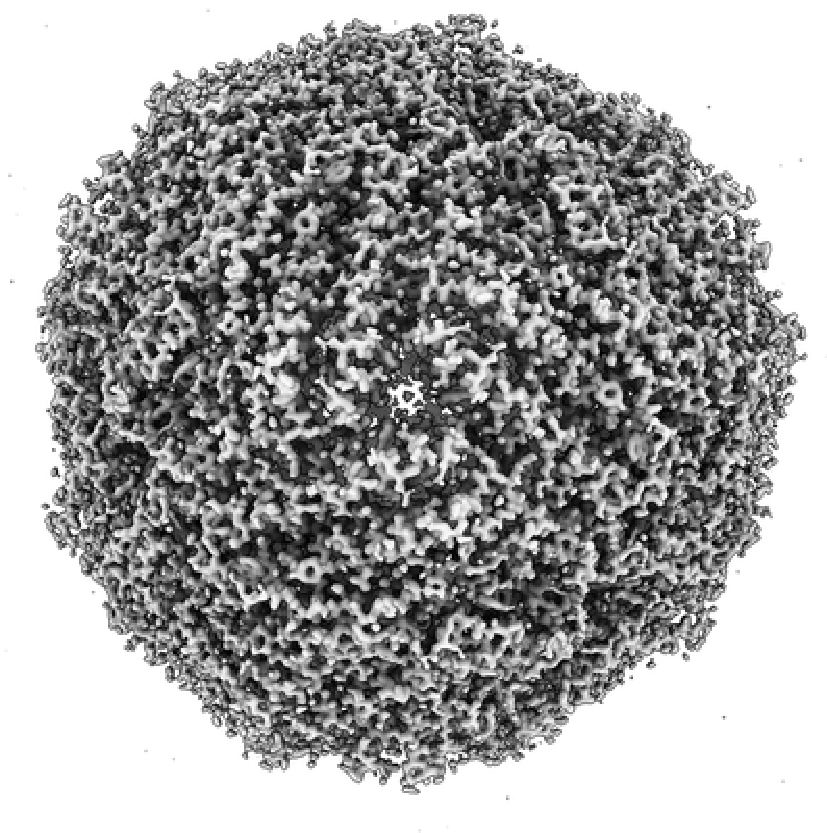
\includegraphics[width=0.50\textwidth]{{images/Cover_apoferritin.pdf}}\\
Cryo-EM map of apoferritin at 1.54 \AA~resolution \footnotesize{(EMD-9865)}
\end{center}

%\vfill % Fill the rest of the page with whitespace
%\begin{minipage}{0.4\textwidth}
\begin{flushright}
 \large
%\emph{Author:}\\
  \textsc{Carlos Oscar S. Sorzano \& Marta Martínez} % Your name
\end{flushright}
%\end{minipage}

\end{titlepage}

\begin{versionhistory}
  \vhEntry{1.0}{11.18.2019}{MM}{Initial draft created for Stanford Image Processing Workshop}
\end{versionhistory}\newpage

%----------------------------------------------------------------------------------------
%	OBJETIVOS
%----------------------------------------------------------------------------------------


\subsection*{Intended audience}
The recent rapid development of single-particle electron cryo-microscopy (cryo-EM) allows structures to be solved by this method at almost atomic resolutions.  Providing a basic introduction to image processing, this tutorial shows the basic workflow aimed at obtaining high-quality density maps from cryo-EM data by using \scipion software framework. %tomography in  electron microscopy with special emphasis in basic image processing. The tutorial requires matlab but does not assume any programing skills. 


\subsection*{We'd like to hear from you}

We have tested and verified the different steps described in this demo
to the best of our knowledge, but since our programs are in continuous
development you may find inaccuracies and errors in this text. Please
let us know about any errors, as well as your suggestions for
future editions, by writing to
scipion@cnb.csic.es.


\subsection*{Requirements}

This tutorial requires, in addition to \scipion, \textit{cryoSPARC2} (\url{https://cryosparc.com/}).

\newpage


%----------------------------------------------------------------------------------------
%	TABLE OF CONTENTS
%----------------------------------------------------------------------------------------

\tableofcontents % Include a table of contents

\newpage % Begins on a new page instead of on the same page as the table of contents


\section{Introduction to Model building}

\subsection*{Definition}
 Model building is the process that allows getting the atomic interpretation of an electron density map. Although a electron density volume can be obtained from different methodologies, in this tutorial we focus in maps obtained by cryo-EM. As an example of these maps, \ffigure{fig:model_building_example} shows the input electron density map (a), as well as the output haemoglobin tetramer atomic model (b) obtained by the model building process. Since high quality atomic structures are essential to accomplish detailed mechanistic studies and to seek inhibitor drugs of macromolecules, the main aim of model building is obtaining reliable structures of these macromolecules. 
 

\begin{figure}[H]
 \centering
 \captionsetup{width=.8\linewidth}  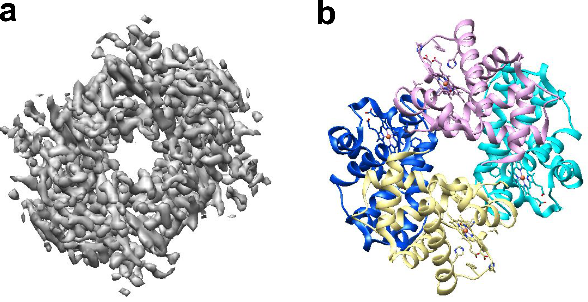
\includegraphics[width=0.6\textwidth]
  {{Images/Fig1.pdf}}
  \caption{Haemoglobin tetramer \citep{khoshouei2017}. a) Electron density map at 3.2\AA\ resolution obtained by Cryo-EM single particle analysis with Volta phase plate. b) Atomic structure model inferred from the electron density volume.}
  \label{fig:model_building_example}
  \end{figure} 
 

\subsection*{Relevance of cryo-EM map resolution}

Model building process is limited by the resolution of the starting cryo-EM density map. The higher the resolution, the more detailed and reliable atomic structure will be obtained. Fortunately, single-particle cryo-EM is undergoing in this decade a resolution revolution that has allowed the structures of macromolecules to be solved at near-atomic resolution. The density map is thus sufficiently resolved to build the atomic model. As a general rule, at resolutions of 4.5\AA\ the molecule backbone can be inferred based on the map alone, and resolutions lower than 4\AA\ allow to trace side chains of some residues. 

 \subsection*{ Model building workflow}
 
 The set of successive tasks aimed to get the atomic interpretation of electron density maps is known as model building workflow. Main steps of the general workflow are detailed from top to bottom in \ffigure{fig:model_building_workflow}. Tasks and tools required are highlighted in green (left side). Before starting those tasks, a detailed study and recruiting of experimental information of the macromolecule itself and similar specimens is recommended. Cryo-EM density map preprocessing is also desirable in order to optimize it by maximizing details and connectivity, as well as extracting the lower asymmetrical element of the starting volume (ASU: asymmetric unit) to save computational resources and facilitate the modeling.
 
 In addition to the map ASU, the workflow considers as input the sequence of each individual structural element (from 1 to n). This sequence is used to get the initial model, \iii{de novo} or by prediction based in structures of homologous sequences. Initial model of each structure element has to be fitted to the volume ASU, and then refined according to the density of this map fraction. Refinement in real and/or reciprocal spaces are included in the workflow. Once refined, the geometry of each individual structure has to be validated regarding the starting volume. The last two steps of refinement and validation will be applied globally to the whole set of structures contained in that map ASU to avoid forbidden steric overlaps among them. Borders between adjacent unit cells will be checked similarly in the reconstruction of the whole atomic structure. 
 
 In this tutorial, we show how to obtain an atomic model using a reference homologous structure.
 
% of model building every step of the general workflow will be considered, except the $de novo$ modeling step because the appropriate tools to accomplish this type of modeling are not still implemented in \scipion. 
 
\begin{figure}[H]
 \centering
 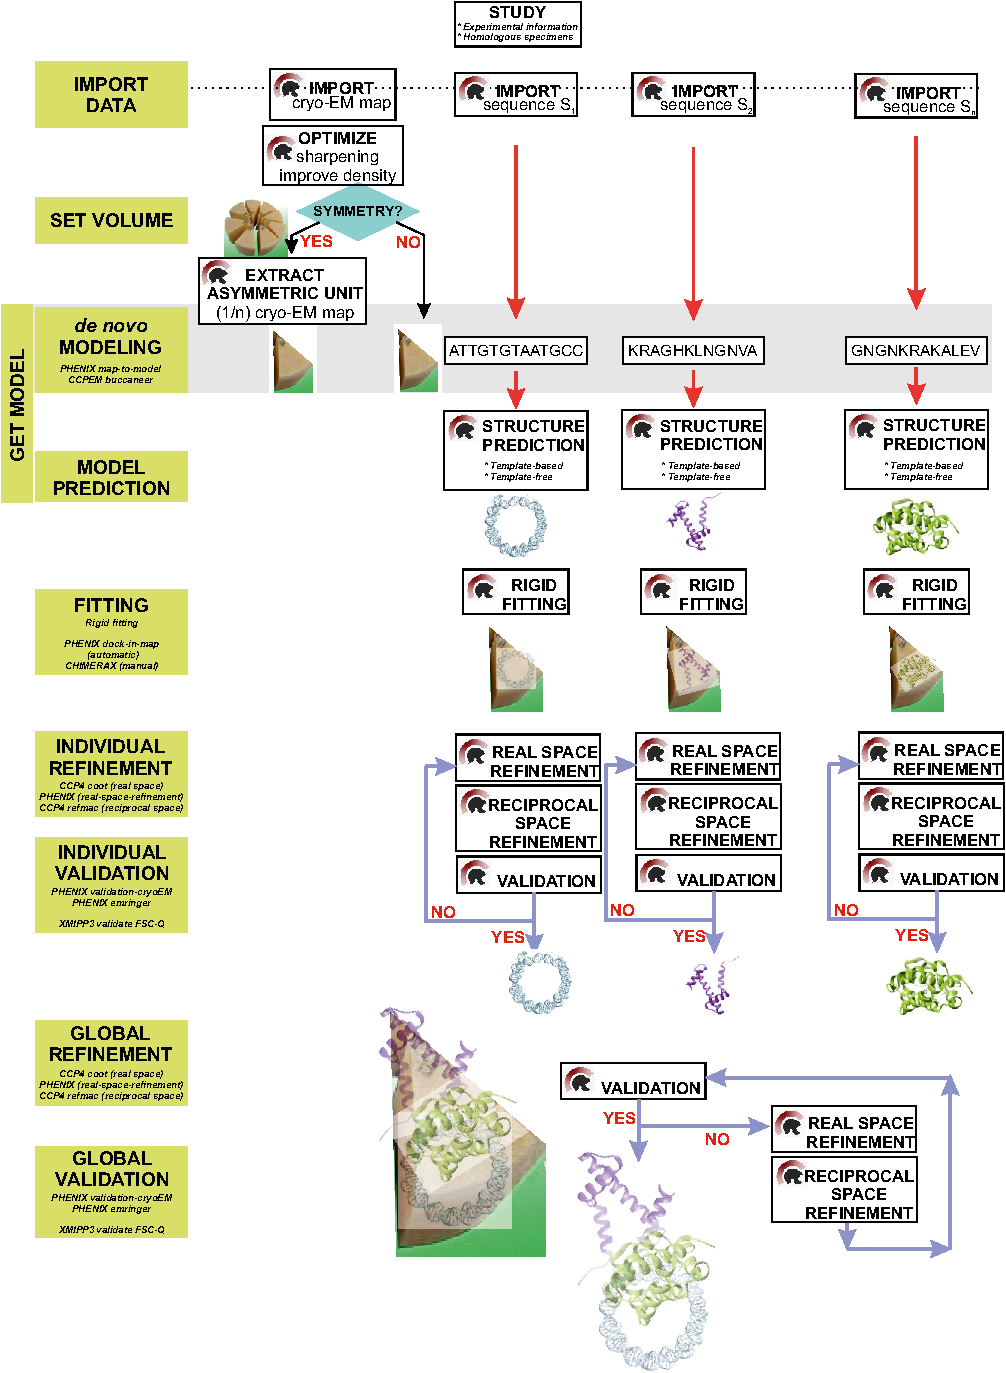
\includegraphics[width=0.95\textwidth]
  {{Images/Fig2.pdf}}
  \caption{General Model Building Workflow.}
  \label{fig:model_building_workflow}
  \end{figure} 
  


\section{Problem to solve: Apoferritin}

Ferritins are iron storage metalloproteins ubiquitously distributed among living organisms. These proteins are involved in iron metabolism in many different types of cells, and play a relevant dual role both in iron detoxification and iron reserve. The ferritin's architecture, similar to a spherical shell, is highly conserved in bacteria, plants and animals, and it allows to accumulate high amounts of Fe(III) atoms (up to 4000 per molecule). \\

The highly stable iron-free shell is known as apoferritin. Mammalian apoferritins are heteromeric molecules, constituted by 24 monomers structurally equivalent that surround the central cavity. Among these monomers, variable proportions of two types of subunits with different properties, H (heavy) and L (light), can be found. The tissues involved in iron storage contain higher proportion of L chains, whereas the tissues that require higher protection against oxidation, such as heart or brain, have a higher content of H chains. Unlike L chains, H chains display ferroxidase catalytic activity, necessary to oxidize Fe(II) to Fe(III). Concerning the structure of each subunit, it is constituted by 4 long helices, a fifth smaller helix and an additional extended loop. The dinuclear iron site, or ferroxidase site, is located in the center of the four helix bundle.\\

This tutorial will guide us in the building process of the mouse apoferritin 3D map using the \scipion framework (\ffigure{fig:workflow_pdf}). As starting input data, we are going to use the \ttt{EMPIAR ID: 10248} data, obtained from mouse heavy chain apoferritin. This cryo-EM data allowed to generate the 3D map \ttt{EMD-9865} at 1.54 \AA\ resolution \citep{hamaguchi2019}. The most recent atomic structure of mouse apoferritin, homo 24-mer of ferritin heavy chain with octahedral symmetry, was also obtained from cryo\-EM data at 1.84 \AA\ (\ttt{PDB ID: 6S61}). The 24 monomers of this metal binding protein are ligated to 6 Fe(III) and 24 Zn(II) ions.

\subsection*{Apoferritin processing workflow in \scipion}
\begin{figure}[H]
  \centering
  \captionsetup{width=.8\linewidth} 
  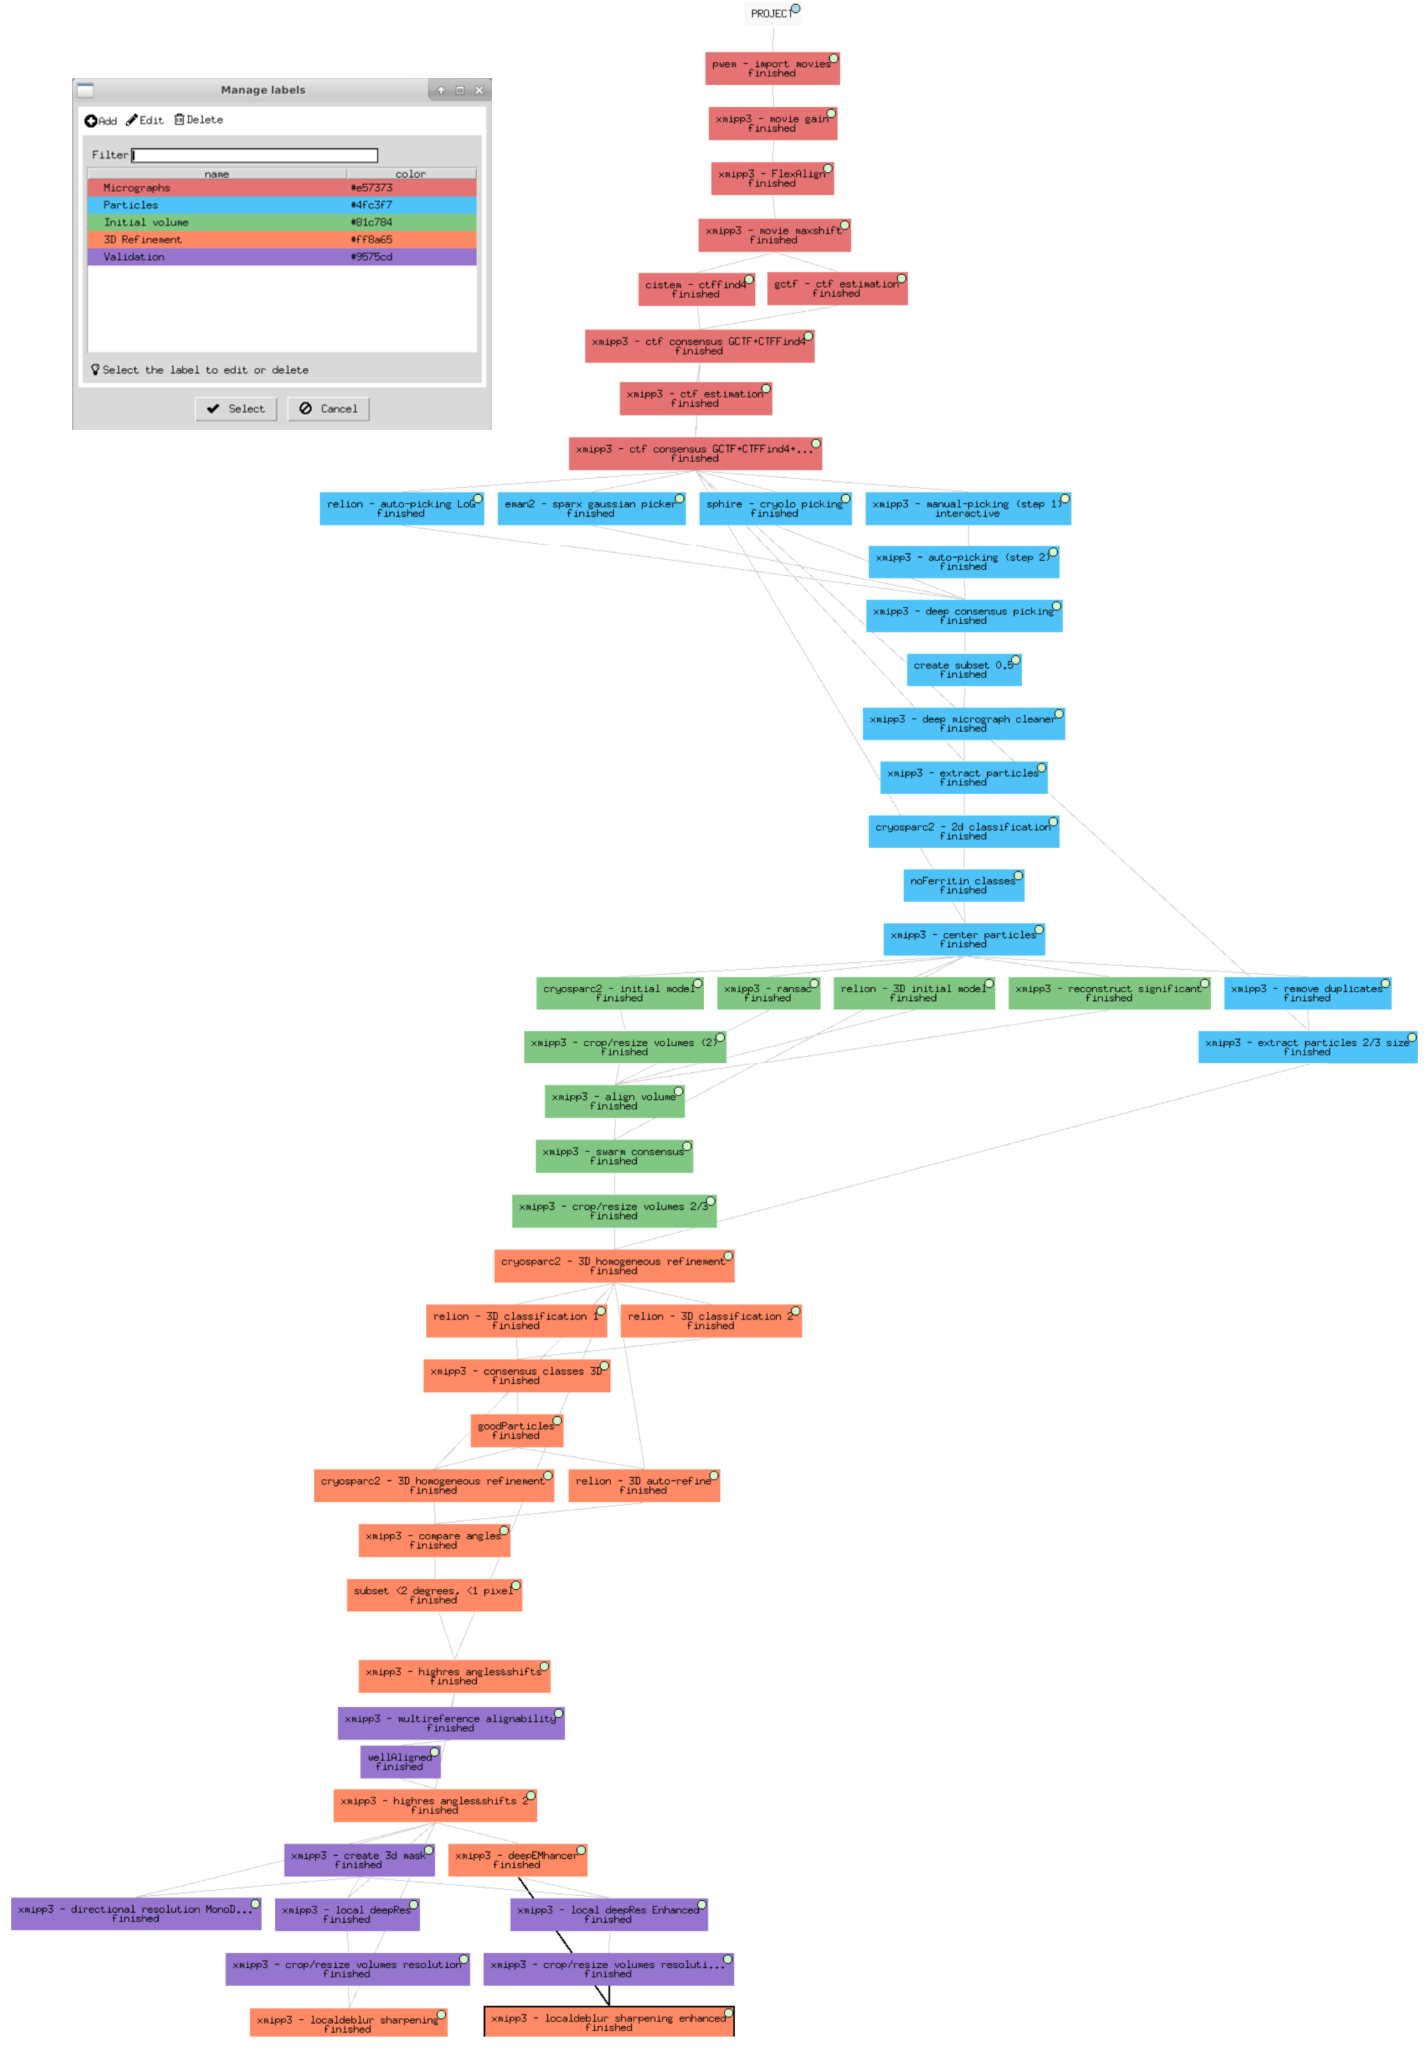
\includegraphics[width=0.95\textwidth]
  {images/workflow1.pdf}
  \caption{Apoferritin processing workflow.}
  \label{fig:workflow_pdf}
  \end{figure}







\section{From movies to micrographs}
 \begin{figure}[H]
  \centering
  \captionsetup{width=.8\linewidth} 
  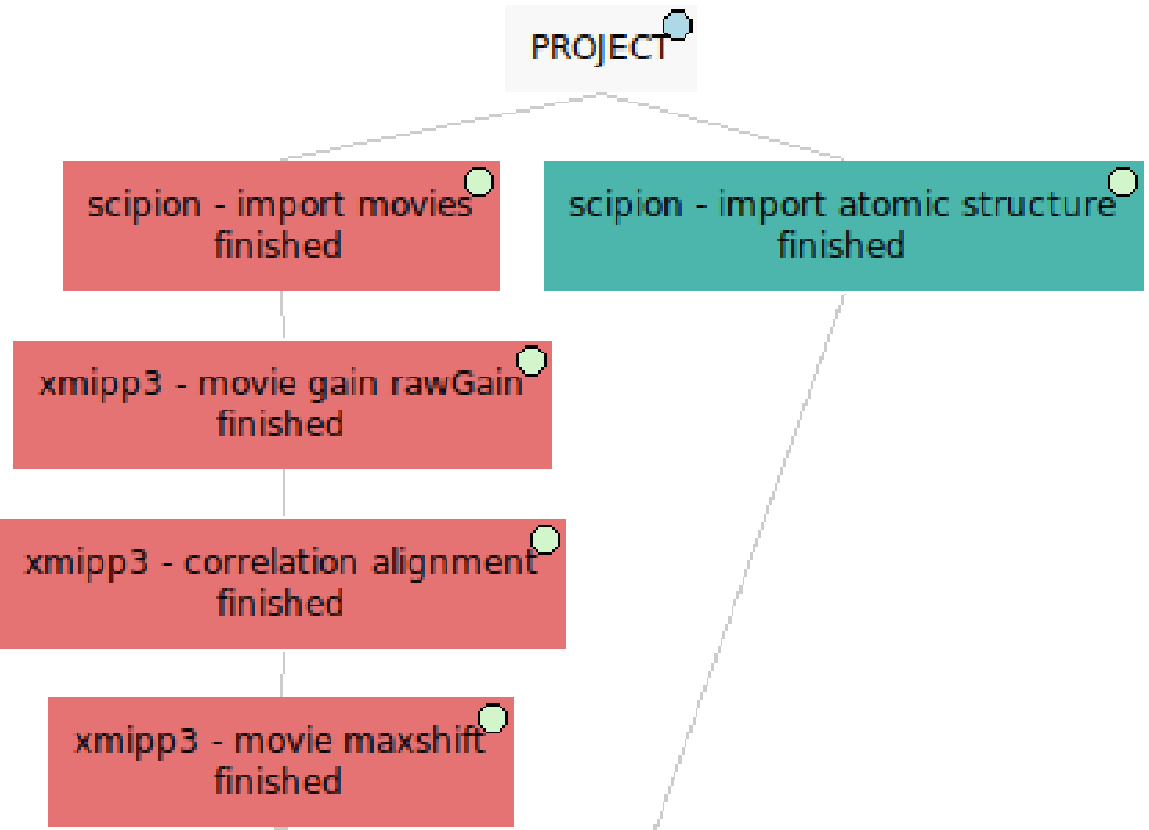
\includegraphics[width=0.65\textwidth]
  {{images/workflow_1.pdf}}
  \caption{From movies to micrographs workflow.}
  \label{fig:workflow_1}
  \end{figure}

 \subsection*{Import movies}
The protocol \scommand{scipion-import movies} allows to download the mouse apoferritin cryo-EM data in \scipion. The protocol form with parameters can be seen in \ffigure{fig:import_movies}. With this protocol, besides the set of movies, located in the Data folder, acquisition parameters such as accelerating voltage, spherical aberration and sample rate, will be registered in your \scipion project. 
 
 \begin{figure}[H]
  \centering
  \captionsetup{width=.8\linewidth} 
  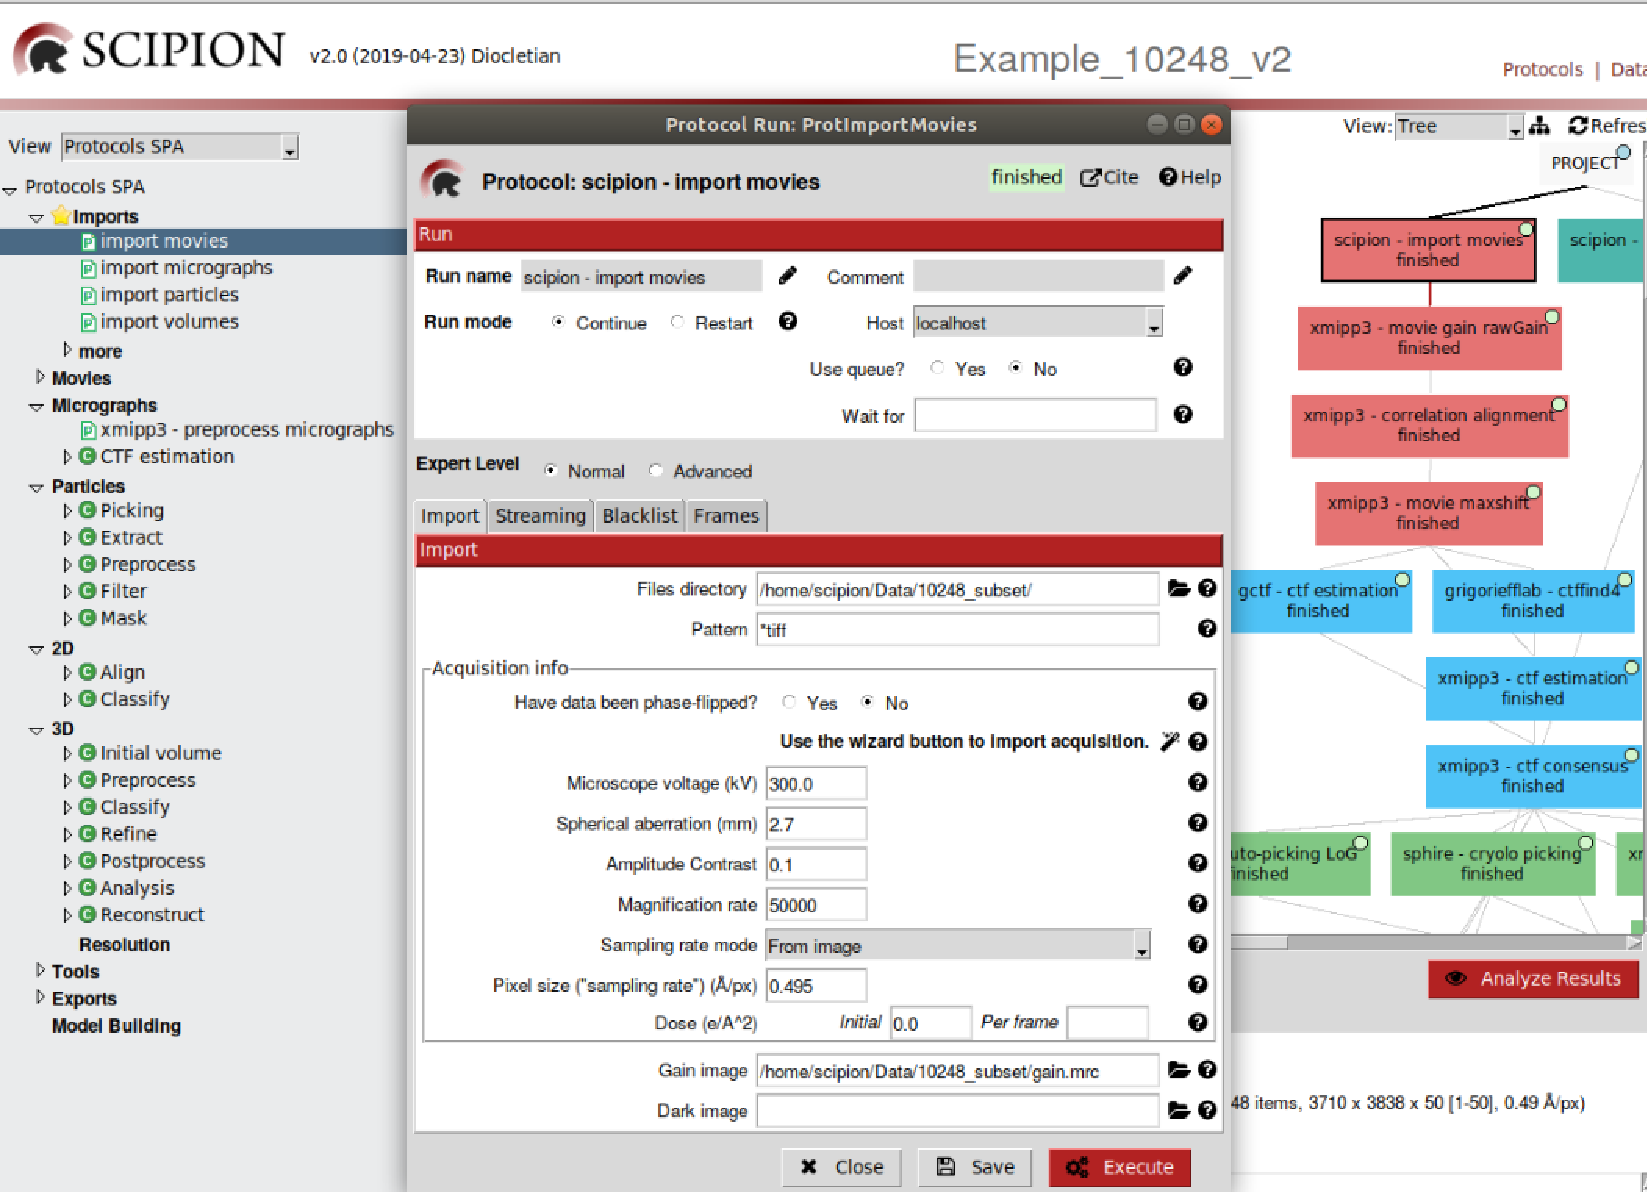
\includegraphics[width=0.95\textwidth]
  {{images/import_movies.pdf}}
  \caption{Filling in the protocol to import cryo-EM data.}
  \label{fig:import_movies}
  \end{figure}
  
After executing this protocol, we can visualize the list of 48 movies imported to the project by pressing \scommand{Analyze Results}. Each movie contains 50 frames with size 3710 pixels x 3838 pixels. Frames contained in each movie can be visualized by right-clicking each entry.
 
 \subsection*{Computation of movie gain}
 
The protocol \scommand{xmipp3-movie gain} is used to compute the movie gain (\ffigure{fig:movie_gain}). Two movie gains will be computed: 1) Without applying the input gain, to orientate the input movie gain; 2) Applying the input gain to estimate the residual movie gain.

\begin{figure}[H]
  \centering
  \captionsetup{width=.8\linewidth} 
  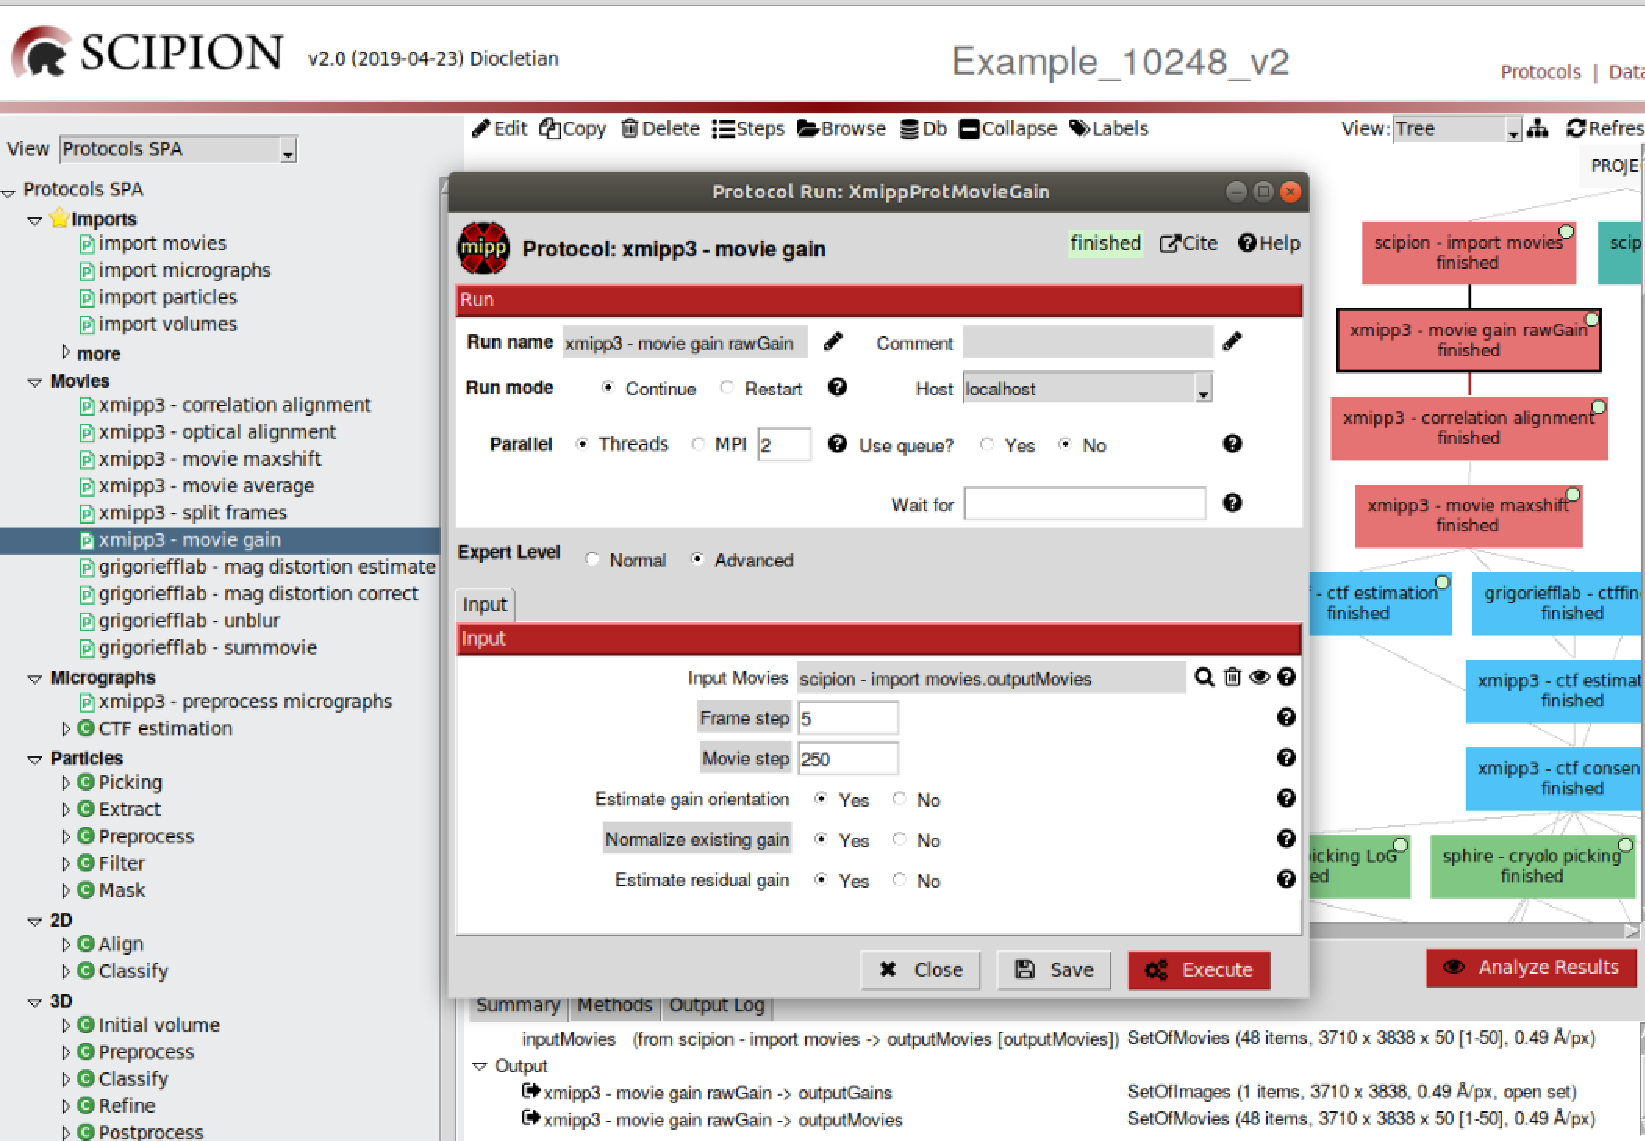
\includegraphics[width=0.95\textwidth]
  {{images/movie_gain.pdf}}
  \caption{Completing the protocol to compute the movie gain.}
  \label{fig:movie_gain}
  \end{figure}
 
After executing this protocol, by pressing \scommand{Analyze Results} we can visualize the image of the gain computed. None of the movie gains computed moves forward the protocol output.

 \subsection*{Movie alignment}
In order to correct BIM-induced image blurring and restore important high resolution information, the stack of individual frames contained in each movie needs to be aligned. Only one image will be generated, and this image is called micrograph. Although in \scipion we have integrated several protocols to perform global and local alignment, in this tutorial we are going to use \scommand{xmipp3-correlation alignment}. We have completed the params of this protocol in \ffigure{fig:correlation_alignment}.

\begin{figure}[H]
  \centering
  \captionsetup{width=.8\linewidth} 
  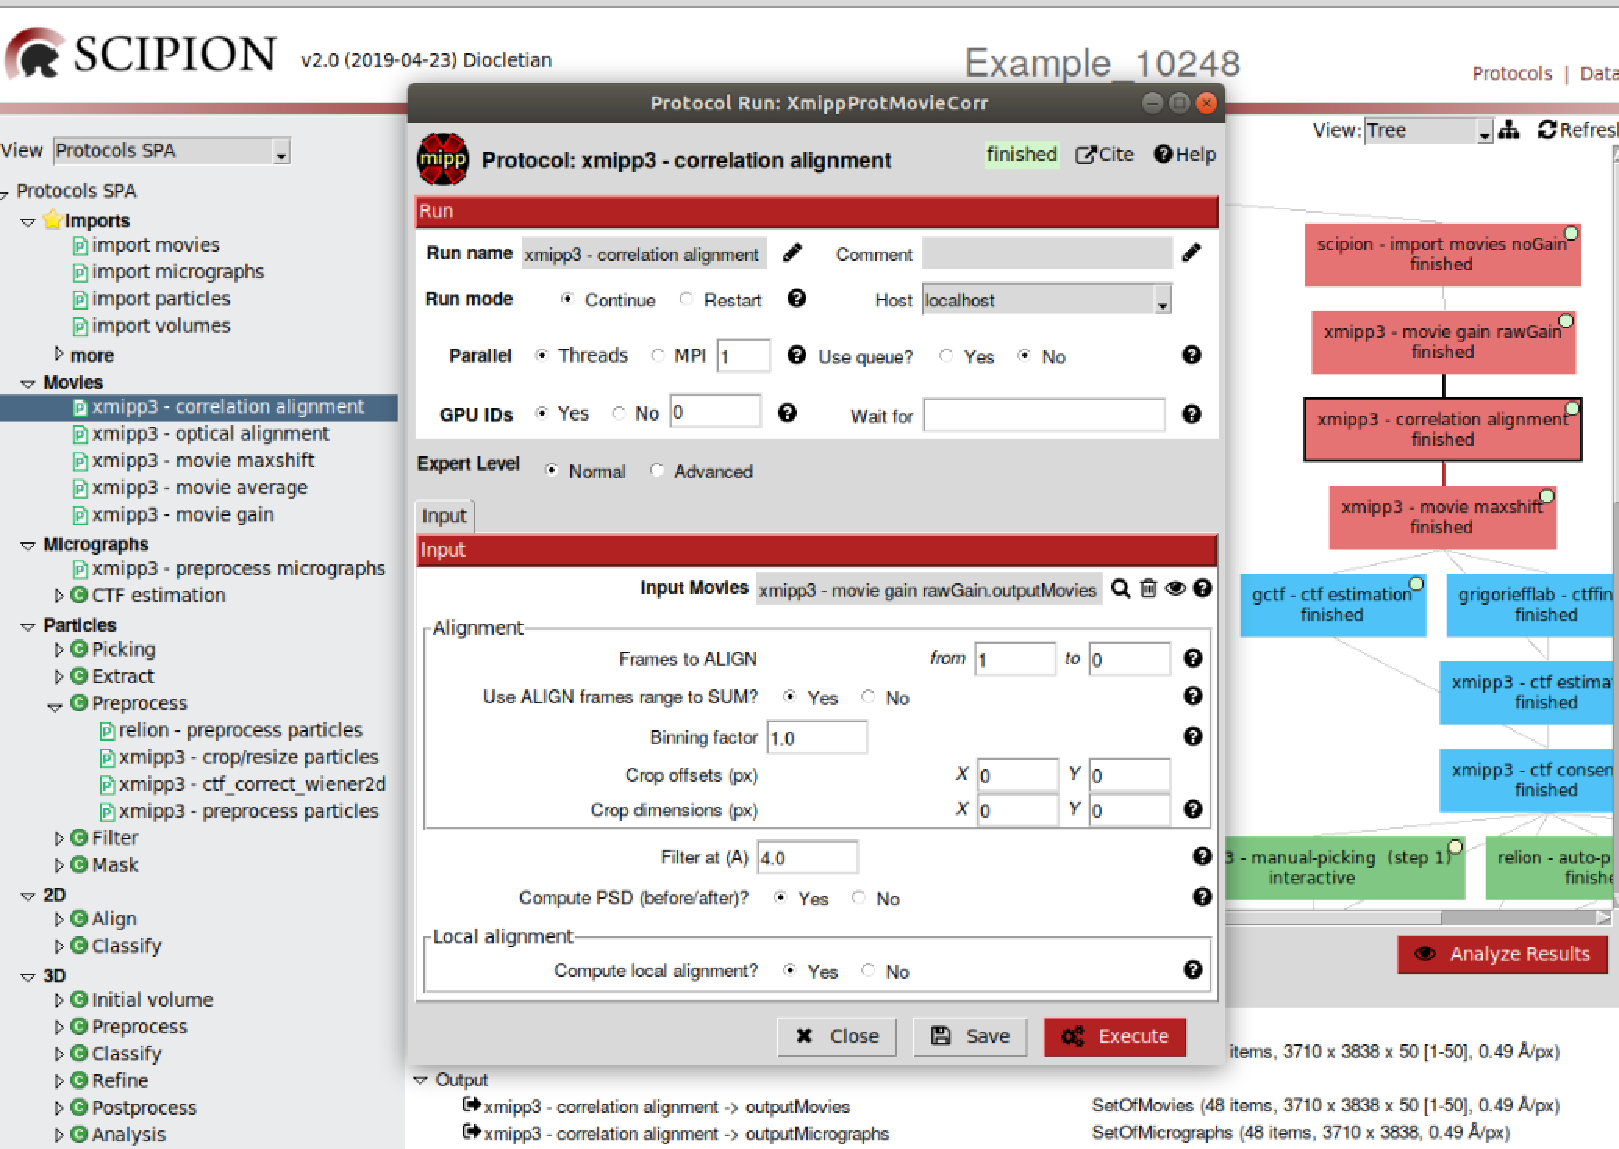
\includegraphics[width=0.95\textwidth]
  {{images/correlation_alignment.pdf}}
  \caption{Filling in the protocol to align the frames of each movie.}
  \label{fig:correlation_alignment}
  \end{figure}
  
When the execution of this protocol finishes, we can observe the list of the set of 48 resulting micrographs by pressing \scommand{Analyze Results}. The first column contains composite images with half of the PSD of the unaligned micrograph (left side) and half of the PSD of the aligned one (right side). The plots in the second column reflect accumulated shifts of the movie frames. The name of each resulting micrograph appears in the third column. Each micrograph included in the set generated can be opened for visual inspection by right-clicking its entry. 

\subsection*{Screening of micrographs}

Since some of the micrographs generated in the previous step could derive from movies with high drift among frames, we have added in the processing workflow a step to select only the micrographs originated from movies with allowed drifting values among frames. The protocol \scommand{xmipp3-movie maxshift}, completed in \ffigure{fig:movie_maxshift}, was designed to screen micrographs according maximum shift values. Movies will be rejected if they exceed the maximum shift value among frames, the maximum travel value for the whole movie, or both previous conditions.

\begin{figure}[H]
  \centering
  \captionsetup{width=.8\linewidth} 
  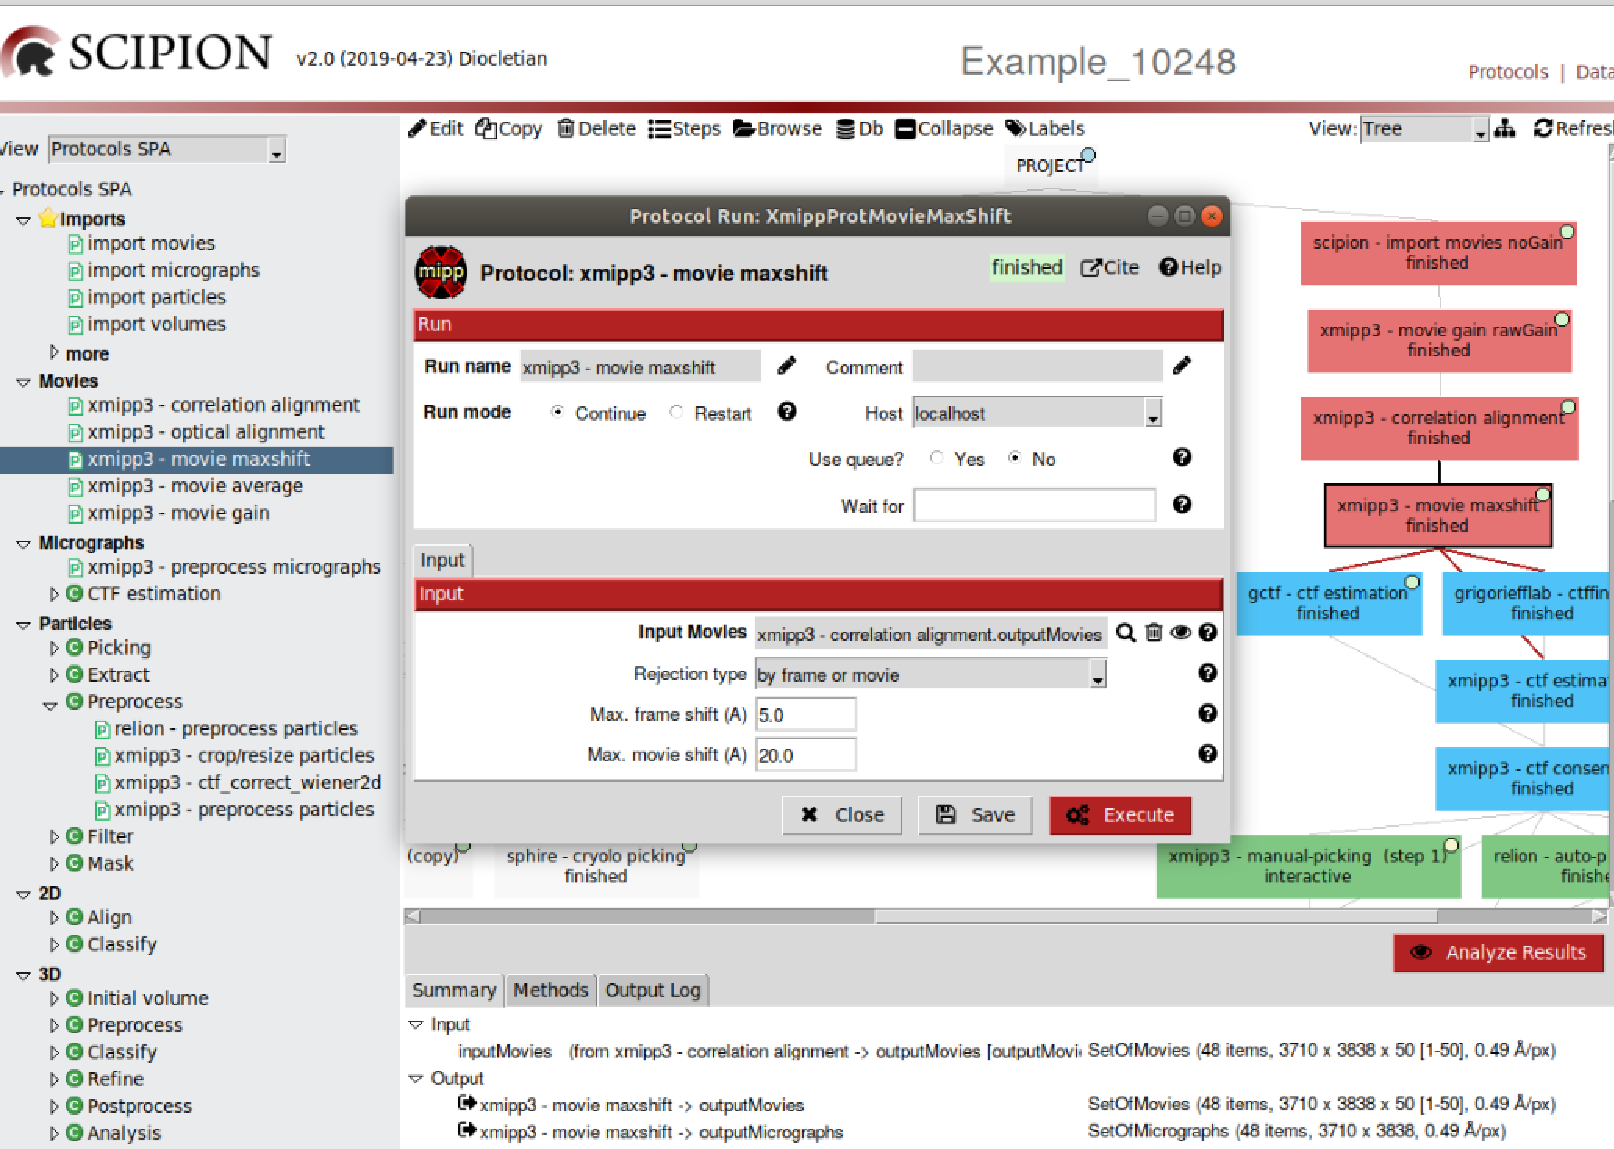
\includegraphics[width=0.95\textwidth]
  {{images/movie_maxshift.pdf}}
  \caption{Completing the protocol to screen the micrographs.}
  \label{fig:movie_maxshift}
  \end{figure}
  
  Once the protocol is executed, both discarded and accepted lists of micrographs can be visualized by pressing \scommand{Analyze Results}. Each micrograph can be opened for visual inspection by right-clicking. In this case, the set of 48 input micrographs have been included in the protocol output. This set will serve as input for further processing steps.

\section{CTF estimation}
 \begin{figure}[H]
  \centering
  \captionsetup{width=.8\linewidth} 
  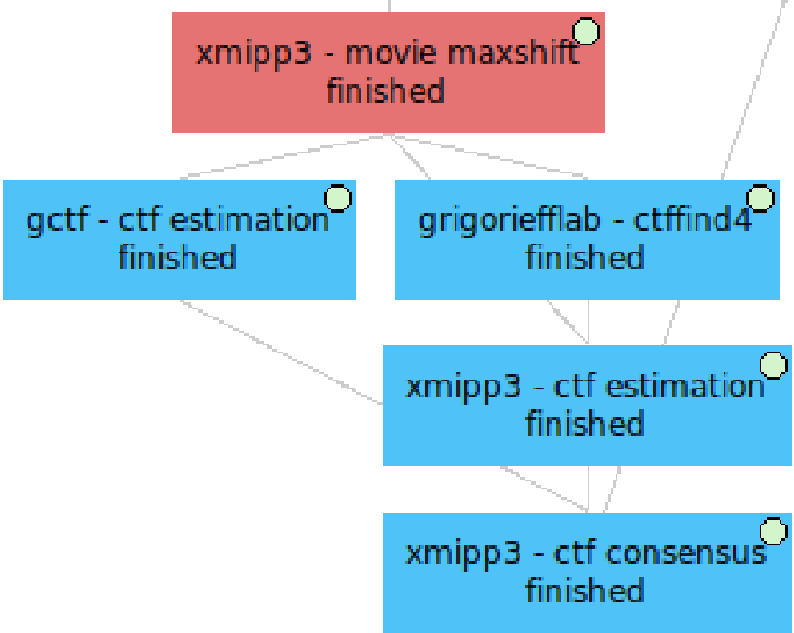
\includegraphics[width=0.55\textwidth]
  {{images/workflow_2.pdf}}
  \caption{CTF estimation workflow (Blue color).}
  \label{fig:workflow_2}
  \end{figure}
Since in focus images of biological specimens embedded in vitreous ice generate very little contrast, we take our movie-frames out of focus, and retrieve systematically distorted images of our specimens. The alteration observed is due to the different transference of contrast for each frequency. In an ideal microscope all the frequencies are transferred with total contrast (+1). In a normal one, some frequencies are transferred with contrast 0 or even -1. The CTF (Contrast transfer function) indicates how much contrast is transferred to the image as a function of the spatial frequency. The estimation of the CTF is the first step to correct it, repair its negative effect and retrieve our specimens undistorted.\\

How to estimate the CTF?\\

Since part of the Fourier components are lost, attenuated or inverted, images of the specimens taken in a non-ideal microscope will appear blurry. We define this blurry effect with the PSF (Point spread function). The effect of the PSF makes that a discrete point in the specimen is reproduced in the image as a thick point surrounded by a variable number of halos. The PSF can be directly estimated from the micrographs and, since the PSF and the CTF are related through the Fourier Transform, by computing the Fourier Transform of the PSF, we can directly estimate the CTF.\\

We count on different protocols to estimate the CTF of the micrographs in \scipion. In this tutorial we are going to use three different algorithms: \ttt{Gctf}\citep{gctf2016}, \ttt{CTFFind4} \citep{ctffind42015} and \ttt{Xmipp CTF estimation} \citep{sorzano2013semiautomatic} executed with protocols \scommand{gctf-ctf estimation} (\ffigure{fig:gctf_ctf_estimation}), \scommand{grigoriefflab-ctffind4}(\ffigure{fig:grigorieff-ctffind4}) and \scommand{xmipp3-ctf estimation}(\ffigure{fig:xmipp3_ctf_estimation}), respectively. Besides of estimating the CTF envelope, this last protocol improves the CTF estimation of \ttt{CTFFind4}. Thus, an additional parameter in this case is the defoci from a \ttt{Previous CTF estimation}. \\

\begin{figure}[H]
  \centering
  \captionsetup{width=.8\linewidth} 
  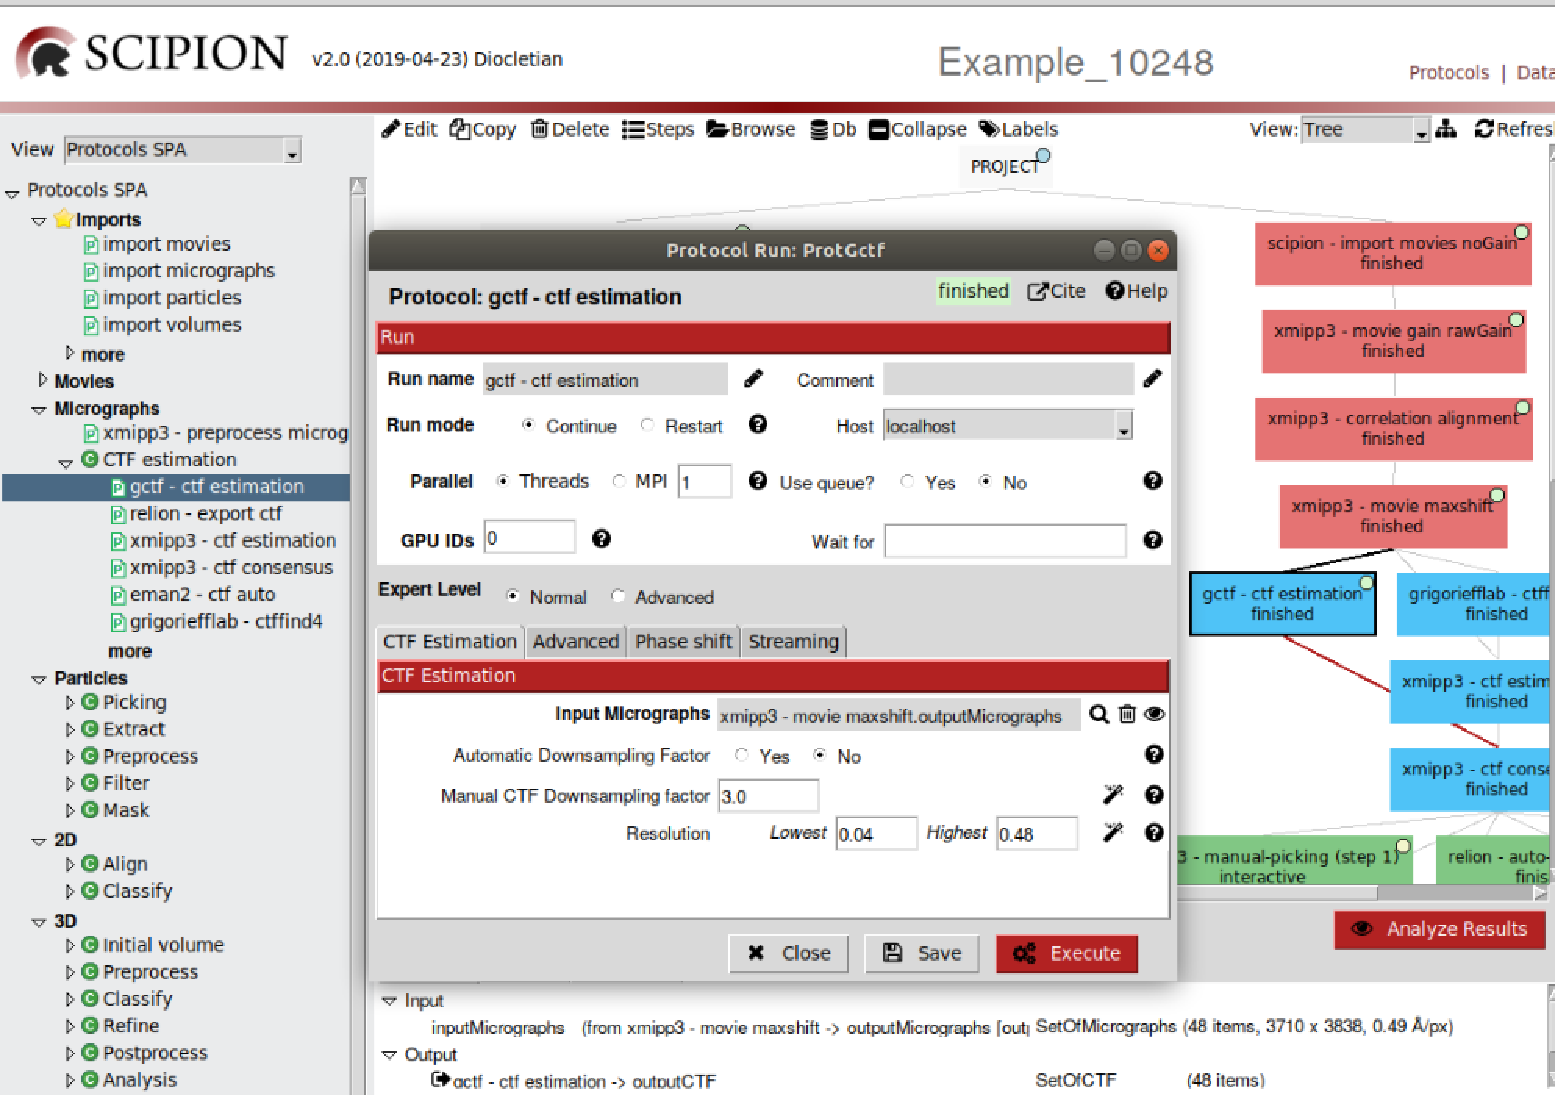
\includegraphics[width=0.95\textwidth]
  {{images/gctf_ctf_estimation.pdf}}
  \caption{Protocol \scommand{gctf-ctf estimation} to compute the CTF.}
  \label{fig:gctf_ctf_estimation}
  \end{figure}
  
  \begin{figure}[H]
  \centering
  \captionsetup{width=.8\linewidth} 
  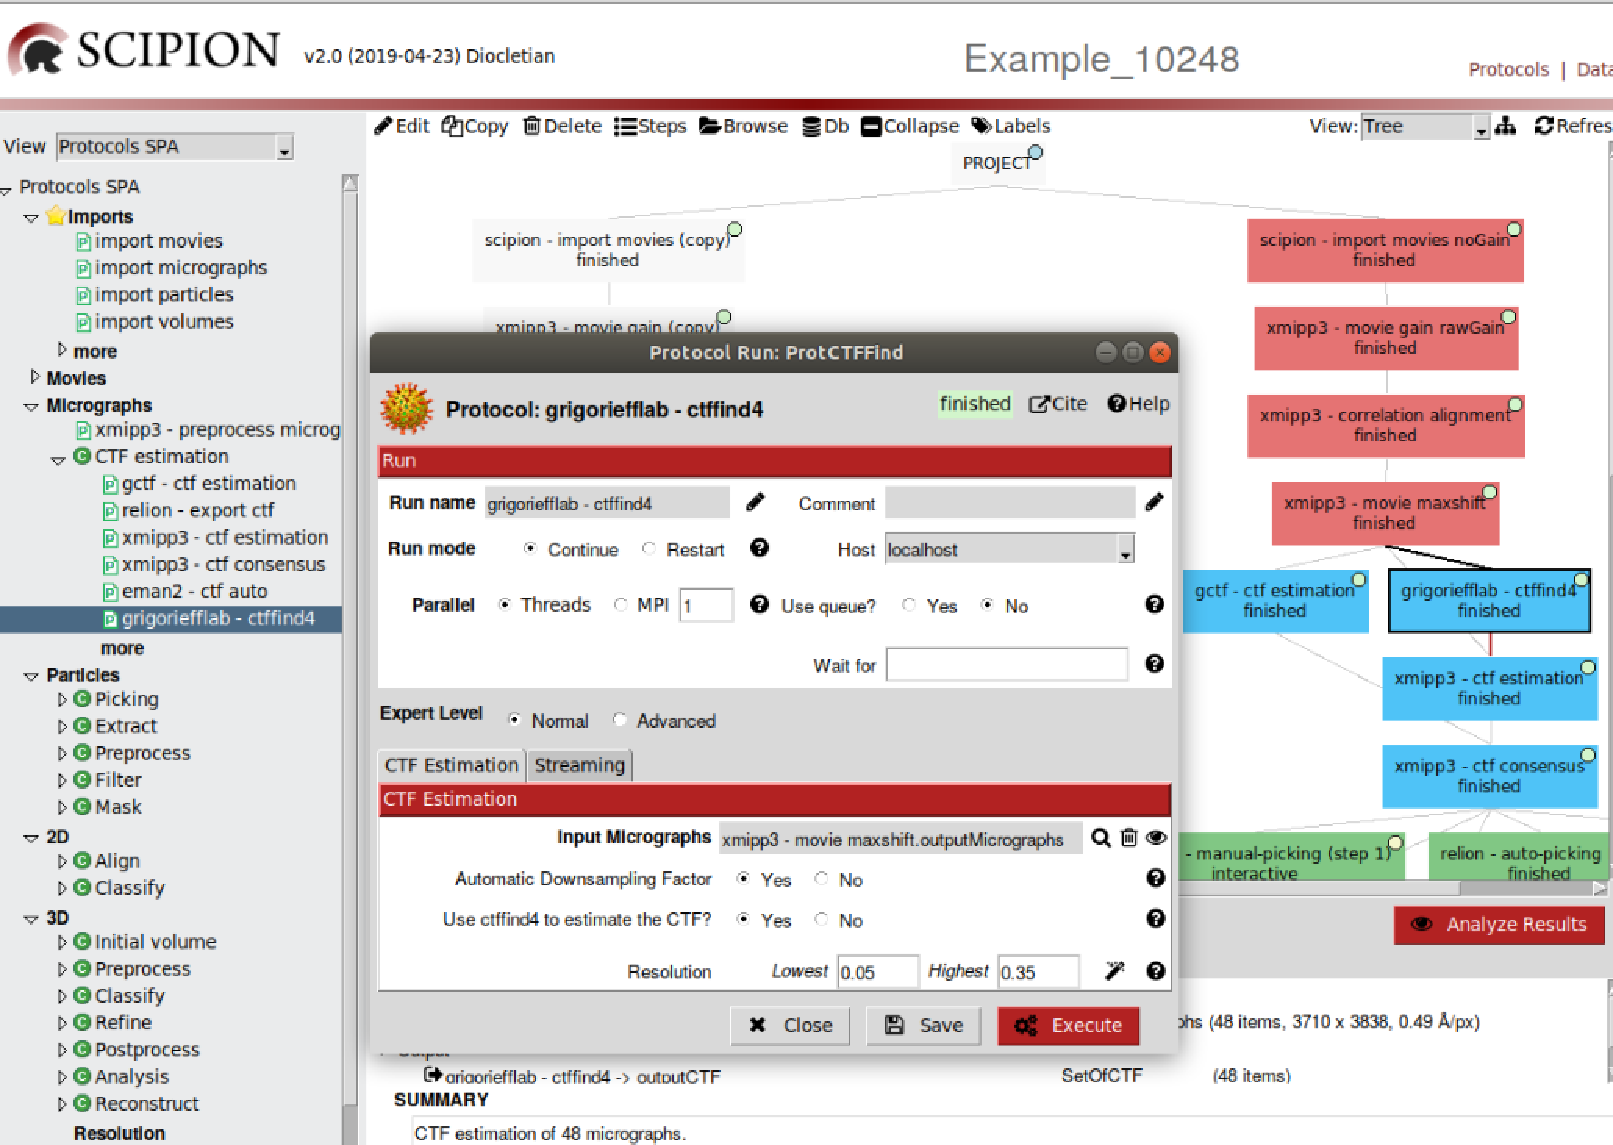
\includegraphics[width=0.95\textwidth]
  {{images/grigorieff_ctffind4.pdf}}
  \caption{Protocol \scommand{grigoriefflab-ctffind4} to compute the CTF.}
  \label{fig:grigorieff-ctffind4}
  \end{figure}
  
  \begin{figure}[H]
  \centering
  \captionsetup{width=.8\linewidth} 
  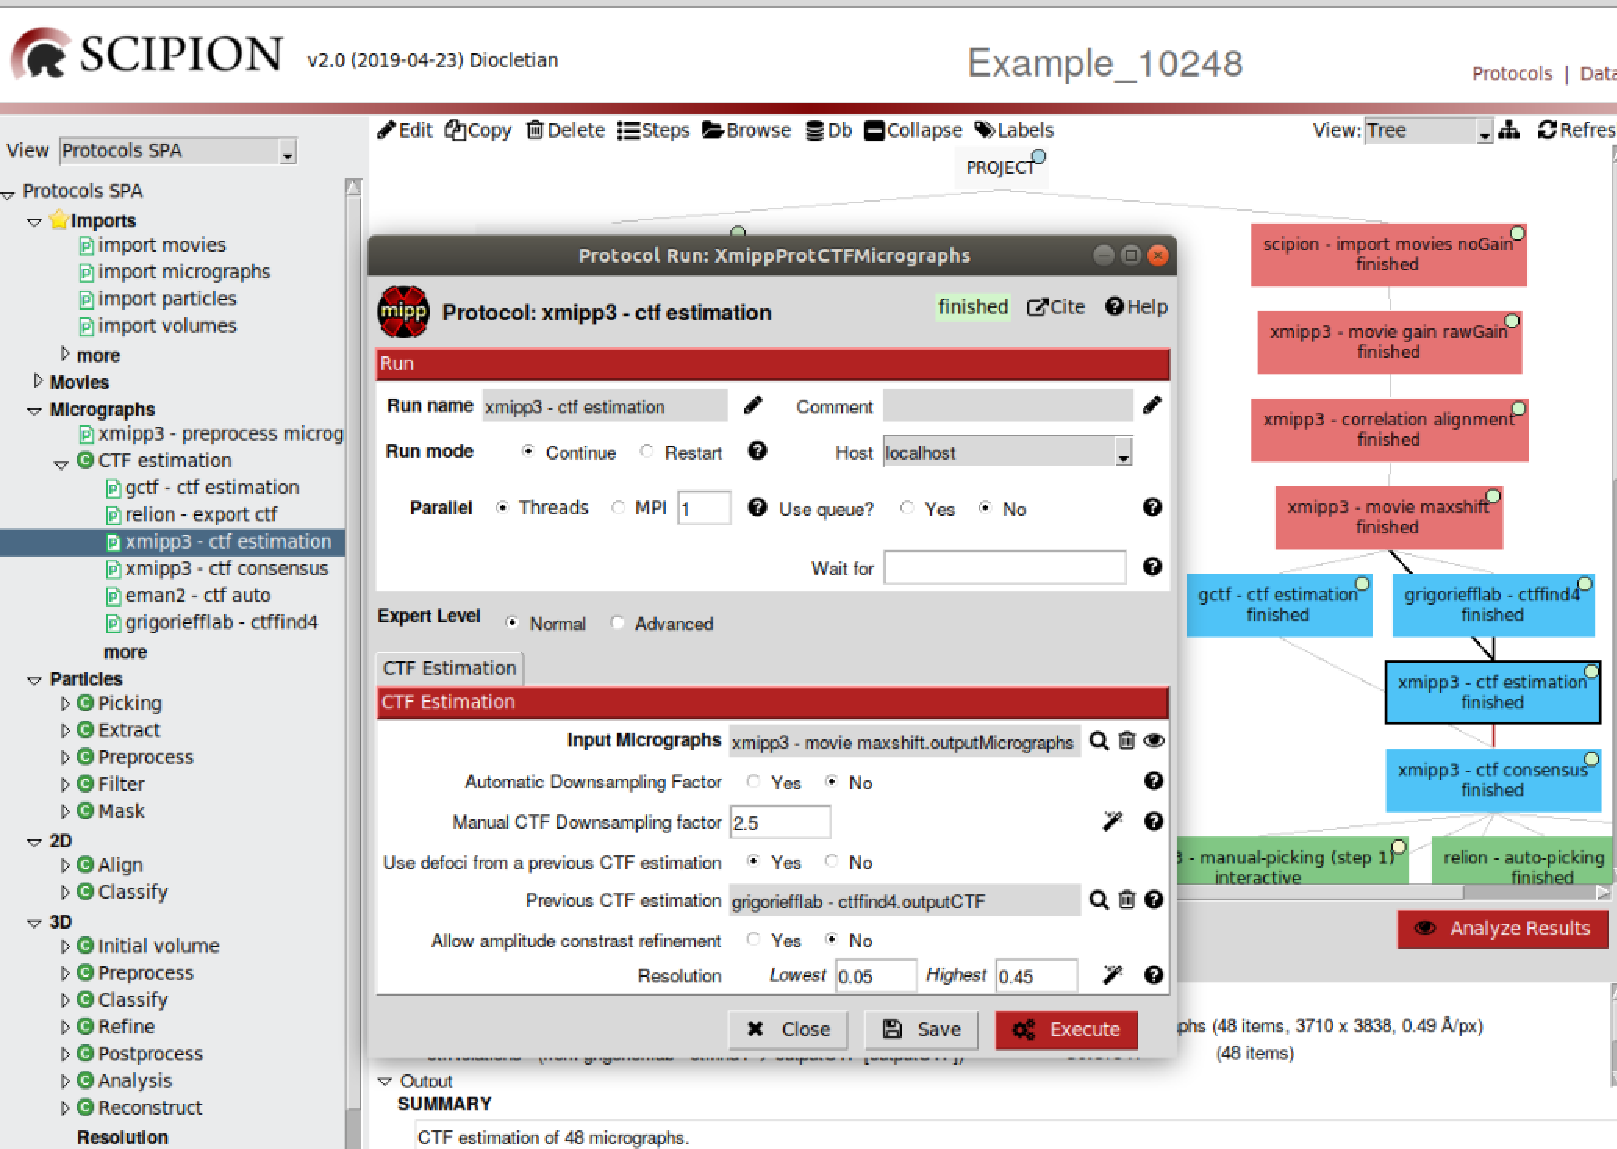
\includegraphics[width=0.95\textwidth]
  {{images/xmipp3-_ctf_estimation.pdf}}
  \caption{Protocol \scommand{xmipp3-ctf estimation} to compute the CTF.}
  \label{fig:xmipp3_ctf_estimation}
  \end{figure}
  
The three algorithms estimate the PSD of the micrographs and the parameters of the CTF (defocus U, defocus V, defocus angle, etc.). They cut micrographs into many smaller images with a desired window size. After that, they compute the Fourier Transform of each image and calculate an average. The three protocols designed to apply the three respective algorithms contain very similar parameters. To estimate the CTF we need to limit the frequency region to be analyzed between the lowest and highest resolution. The frequency domain selected must include all zeros of the CTF. The wizard displayed on the right helps to choose that frequency region.\\

After executing each one of these three protocols, results can be observed by pressing \scommand{Analyze results}. A table will be opened showing the image of the CTF computed of each micrographs, as well as other CTF parameters. CTFs of good micrographs typically display multiple concentric rings extending from the image center towards its edges. Bad micrographs, however, might lack rings or show very few of them that hardly extend from the image center. Micrographs like these will be discarded, likewise micrographs showing strongly asymmetric rings (astigmatic) or rings that attenuate in a particular direction (drifted). To discard a particular micrographs, select it, clik the mouse right button and choose \ttt{Disable}. If you want to see the CTF profile, choose the option \ttt{Show CTF profile}, and a new window will be opened to show the CTF profile. \ttt{Recalculate CTFs} and \ttt{Micrographs} are additional options of \scommand{Analyze results} menu that can be used after selecting specific micrographs. \ttt{Recalculate CTFs} allows to estimate again the CTF when the algorithm has previously failed to find the rings, even they can be seen by eye. The option \ttt{Micrographs} allows to create a new subset of selected micrographs.\\

Concerning some differences among protocols, we remark that micrographs with CTF estimated with \scommand{grigoriefflab-ctffind4} display a hole in the center because, in some cases, they have very much power and avoid appreciate what is underneath. In the particular case of \scommand{xmipp3-ctf estimation} four different images of micrographs are shown. Besides the PSD, this last protocol displays the enhanced PSD, the CTF model by quadrants and half plane.\\

\subsection*{CTF consensus}
The CTF estimation process concludes by applying a consensus protocol to assess differences among the output of the algorithms \ttt{Gctf} and \ttt{Xmipp CTF estimation}. We are going to use \scommand{xmipp3-ctf consensus} to perform this task (\ffigure{fig:xmipp3-ctf_consensus_1}). This protocol allows to screen micrographs according meaningful CTF estimations based on defocus values, astigmatism, resolution and other \ttt{Xmipp} criteria (second tap in the protocol form), which will only be used in case that any of the CTFs computed is estimated by \scommand{xmipp3-ctf estimation}.\\

\begin{figure}[H]
  \centering
  \captionsetup{width=.8\linewidth} 
  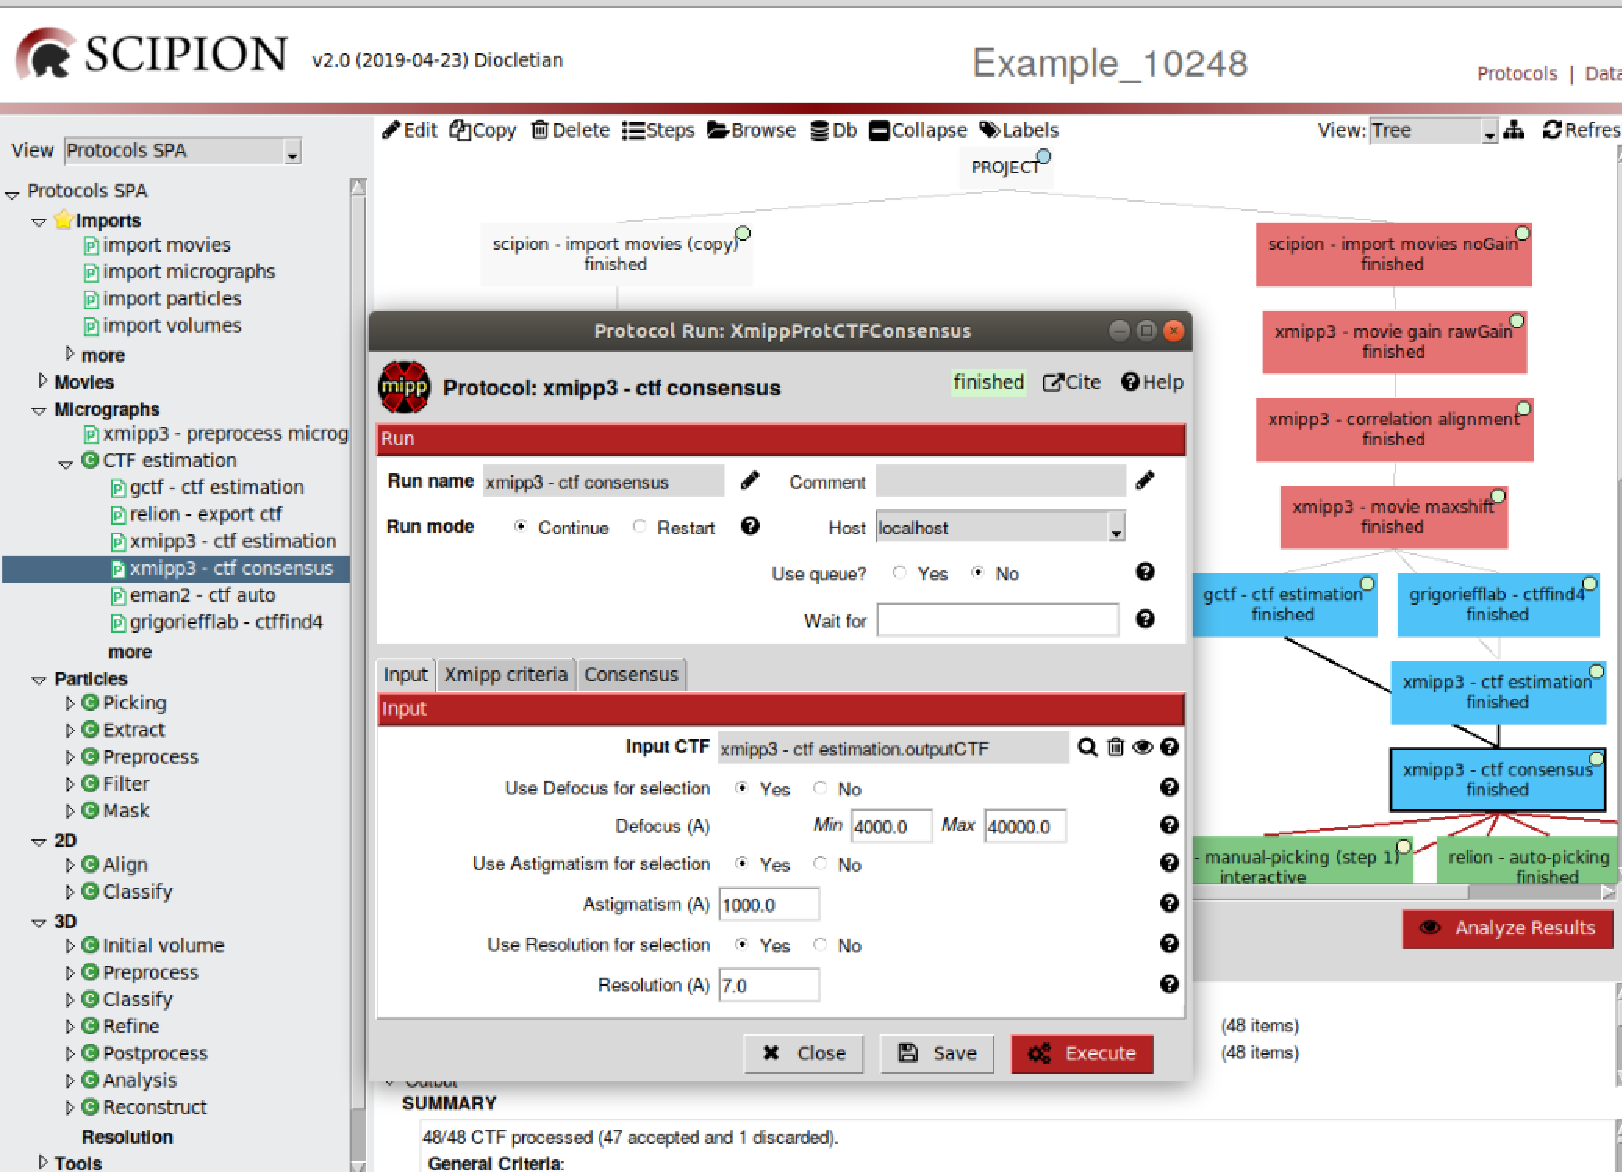
\includegraphics[width=0.95\textwidth]
  {{images/xmipp3-_ctf_consensus_1.pdf}}
  \caption{Filling in the consensus protocol \scommand{xmipp3-ctf consensus}.}
  \label{fig:xmipp3-ctf_consensus_1}
  \end{figure}

In this case we have selected as first input the estimation of the CTF calculated by \scommand{xmipp3-ctf estimation} and as second input the estimation obtained by \scommand{gctf-ctf estimation}. By pressing \scommand{Analyze Results} both accepted (41) and rejected (1) micrographs can be visualized.\\

With the good micrographs we can continue the image processing. The negative effects of the CTF will be corrected in the next steps.

\section{Particle picking}
 \begin{figure}[H]
  \centering
  \captionsetup{width=.8\linewidth} 
  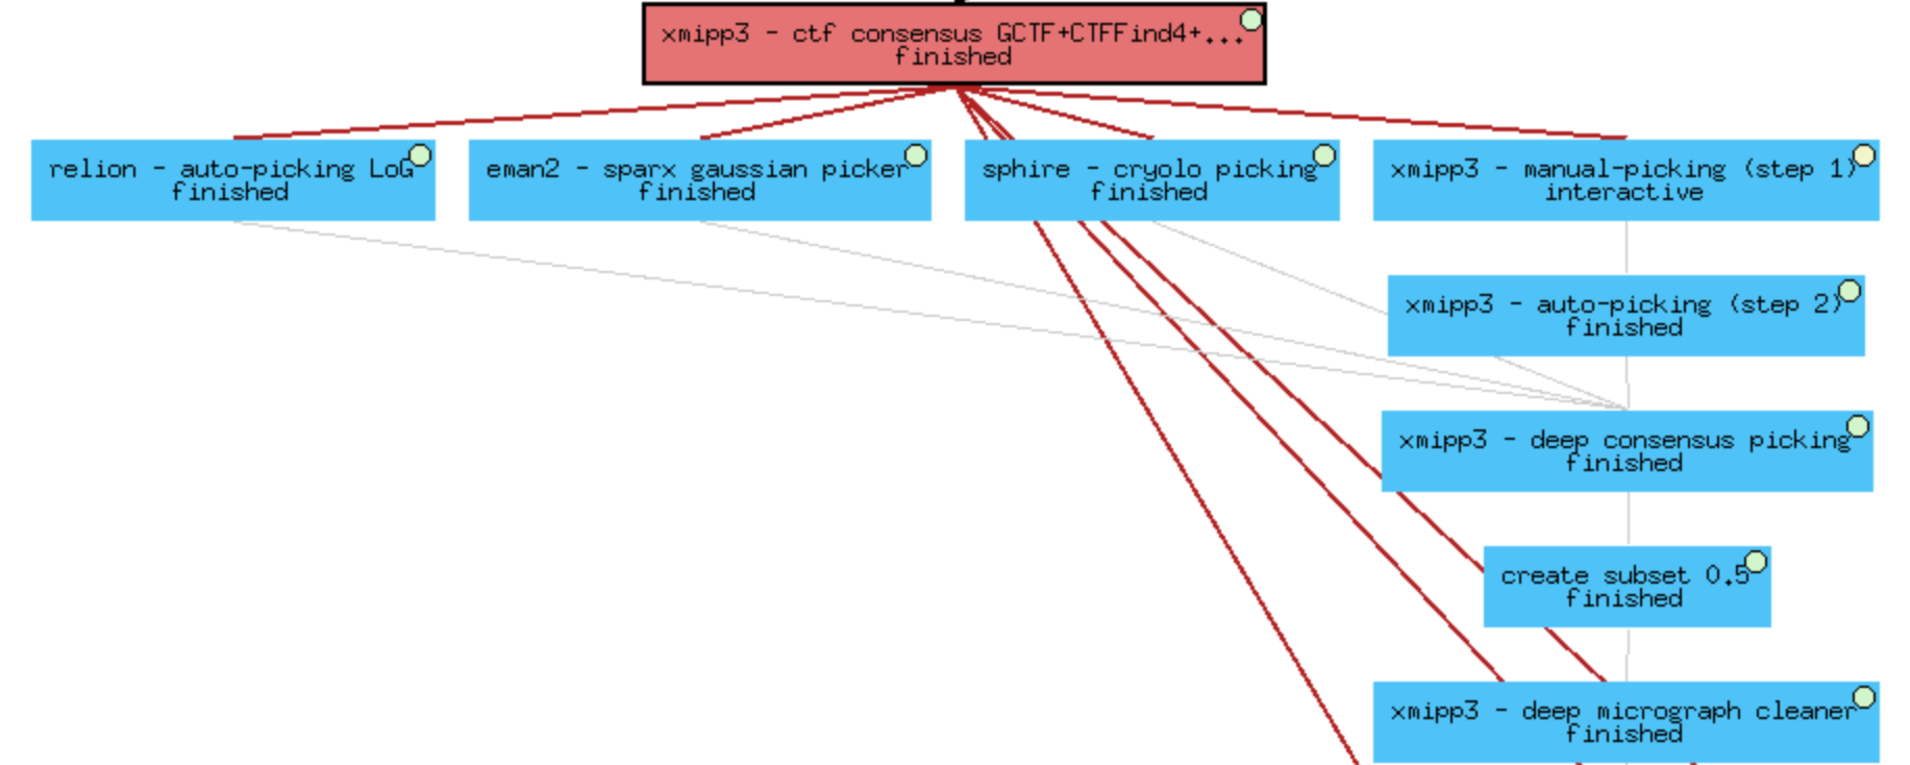
\includegraphics[width=0.75\textwidth]
  {{images/5_workflow3_ParticlePicking.pdf}}
  \caption{Particle picking workflow.}
  \label{fig:workflow_3}
  \end{figure}

Since the reconstruction of the 3D density map of the macromolecule is based on images of individual single particles, the next step is essential in the image processing workflow. With the particle picking step we will retrieve the coordinates of each single particle.\\

Because manual picking can be very tedious, some tools have been designed to help in this task. We have integrated in \scipion different picking tools that can be used individually or in combination to obtain the final coordinates. Currently, we have tools available from \ttt{Eman2}, \ttt{Relion}, \ttt{Bsoft}, \ttt{Sphire} and \ttt{Xmipp}. In this tutorial we are going to use four different protocols that integrate tools from \ttt{Relion} (\scommand{relion-auto-picking LoG} \citep{relion32018}), \ttt{Eman2 (\scommand{eman2-sparx gaussian picker})}, \ttt{Sphire} (\scommand{sphire-cryolo picking} \citep{cryolo2019}) and \ttt{Xmipp} (\scommand{xmipp3- manual-picking (step1)} and \scommand{xmipp3-auto-picking (step 2)} \citep{sorzano2013semiautomatic}). The reason for using several pickers is that, each of them have different properties and different errors which complement the process to have a better estimate.\\

The protocol \scommand{relion-auto-picking LoG} (\ffigure{fig:relion_autopicking}) provides particle coordinates in an automatic way. Together with the 28 input micrographs and the size in pixels for each particle, the protocol form allows to set specific parameters to compute the Laplacian of Gaussian (LoG).

\begin{figure}[H]
  \centering
  \captionsetup{width=.8\linewidth} 
  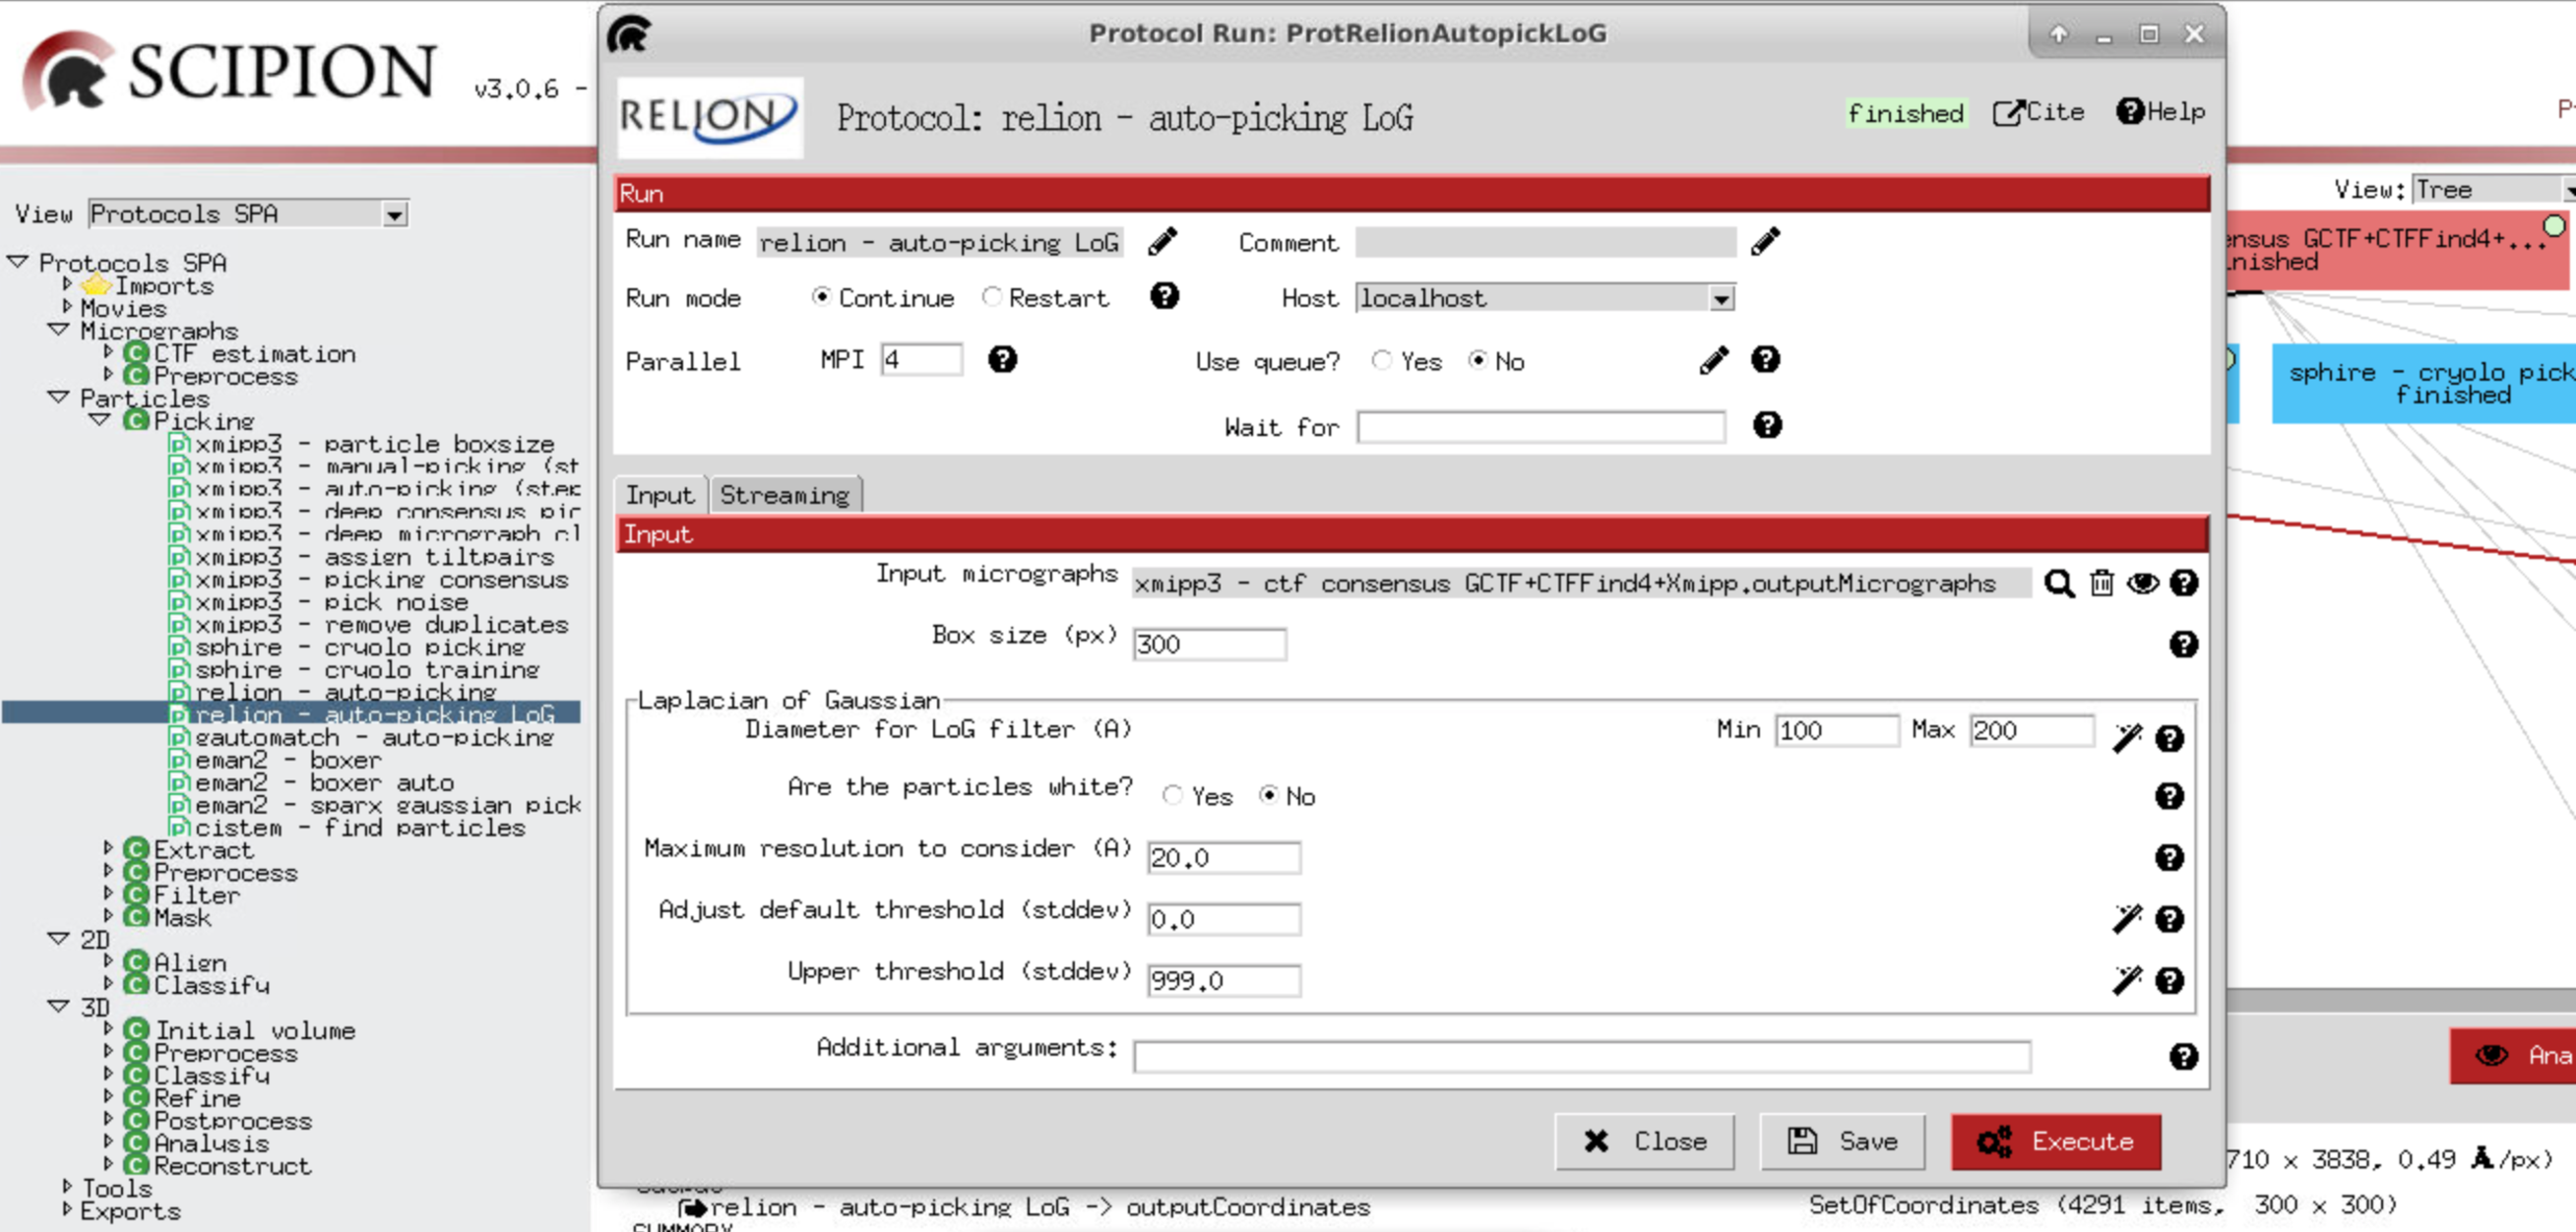
\includegraphics[width=0.95\textwidth]
  {{images/5a_relion_autopickingLog.pdf}}
  \caption{Filling in the protocol 1 \scommand{relion-auto-picking LoG}.}
  \label{fig:relion_autopicking}
  \end{figure}
  
  The protocol \scommand{eman2-sparx gaussian picker} (\ffigure{fig:eman2_sparx}) provides particle coordinates in an automatic way. Similar to Relion, together with the 28 input micrographs, we have to set the size in pixels for each particle, and the width of the Gaussian kernel used for automated particle picking, the protocol allows us to obtain the particles as a set of coordinates.
  
\begin{figure}[H]
  \centering
  \captionsetup{width=.8\linewidth} 
  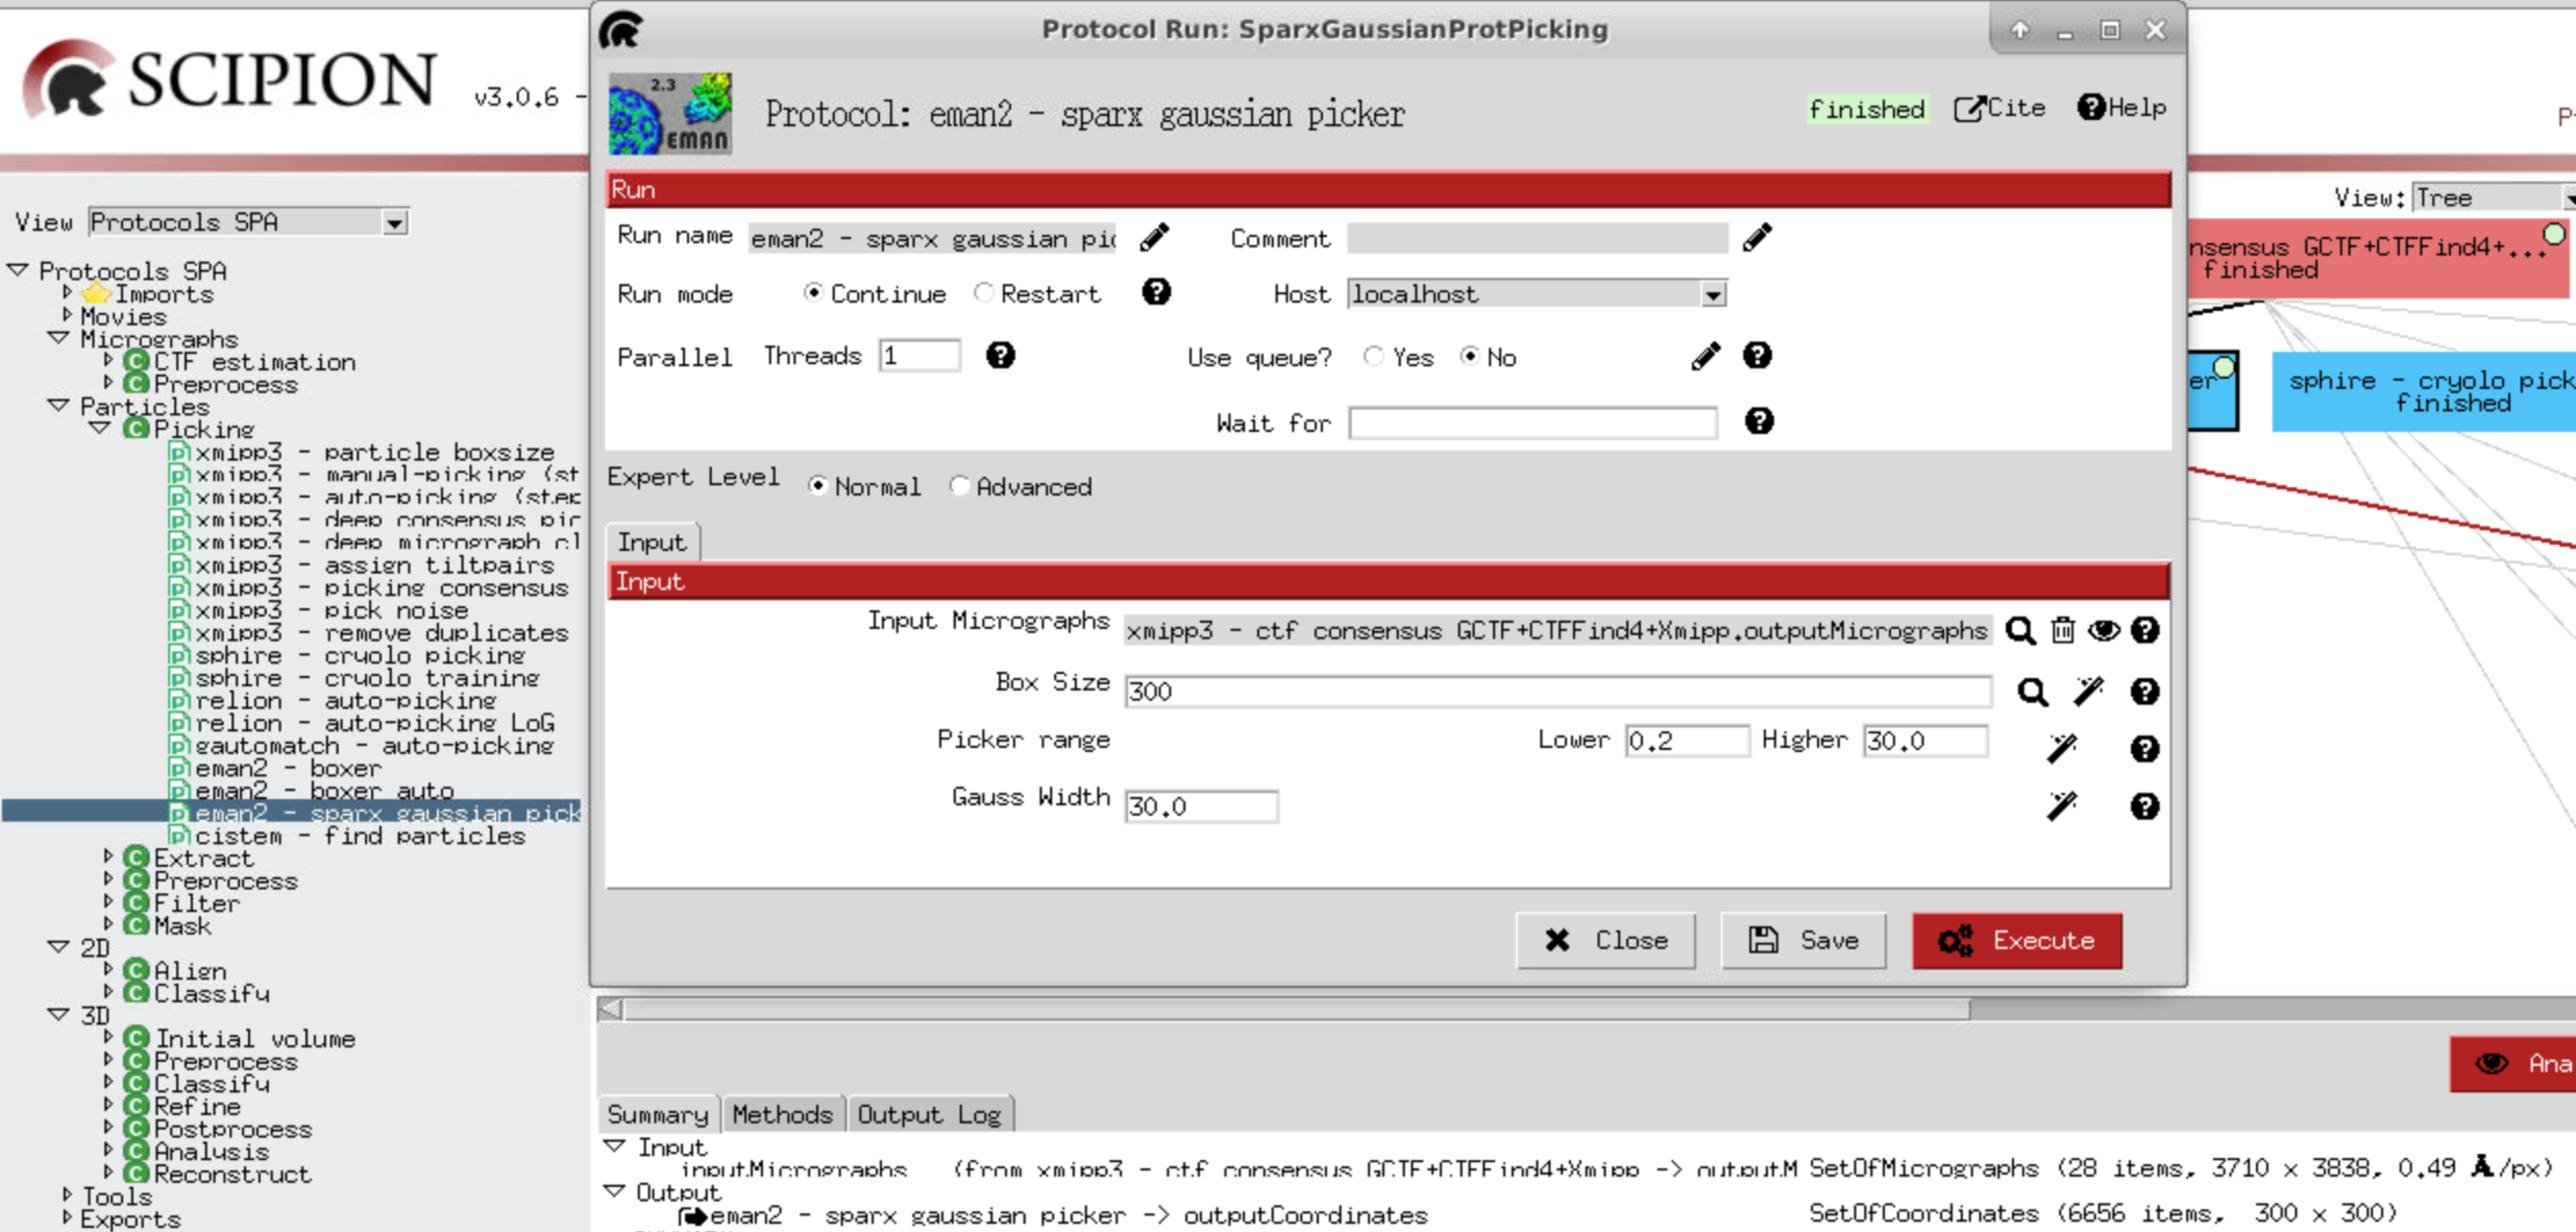
\includegraphics[width=0.95\textwidth]
  {{images/5b_eman2_SparxGaussianPicker.pdf}}
  \caption{Filling in the protocol 2 \scommand{eman2-sparx gaussian picker}.}
  \label{fig:eman2_sparx}
  \end{figure}
  
The protocol \scommand{sphire-cryolo picking} (\ffigure{fig:sphire-cryolo}) integrates a fully automated particle picker based on deep learning. The protocol form also requires the 28 micrographs and the size of particles, and gives you the possibility of using your own network model, obtained in a previous training step, instead of the general one. \ttt{Confidence threshold} allows to perform a more or less conservative picking by increasing or decreasing the value of this param.

\begin{figure}[H]
  \centering
  \captionsetup{width=.8\linewidth} 
  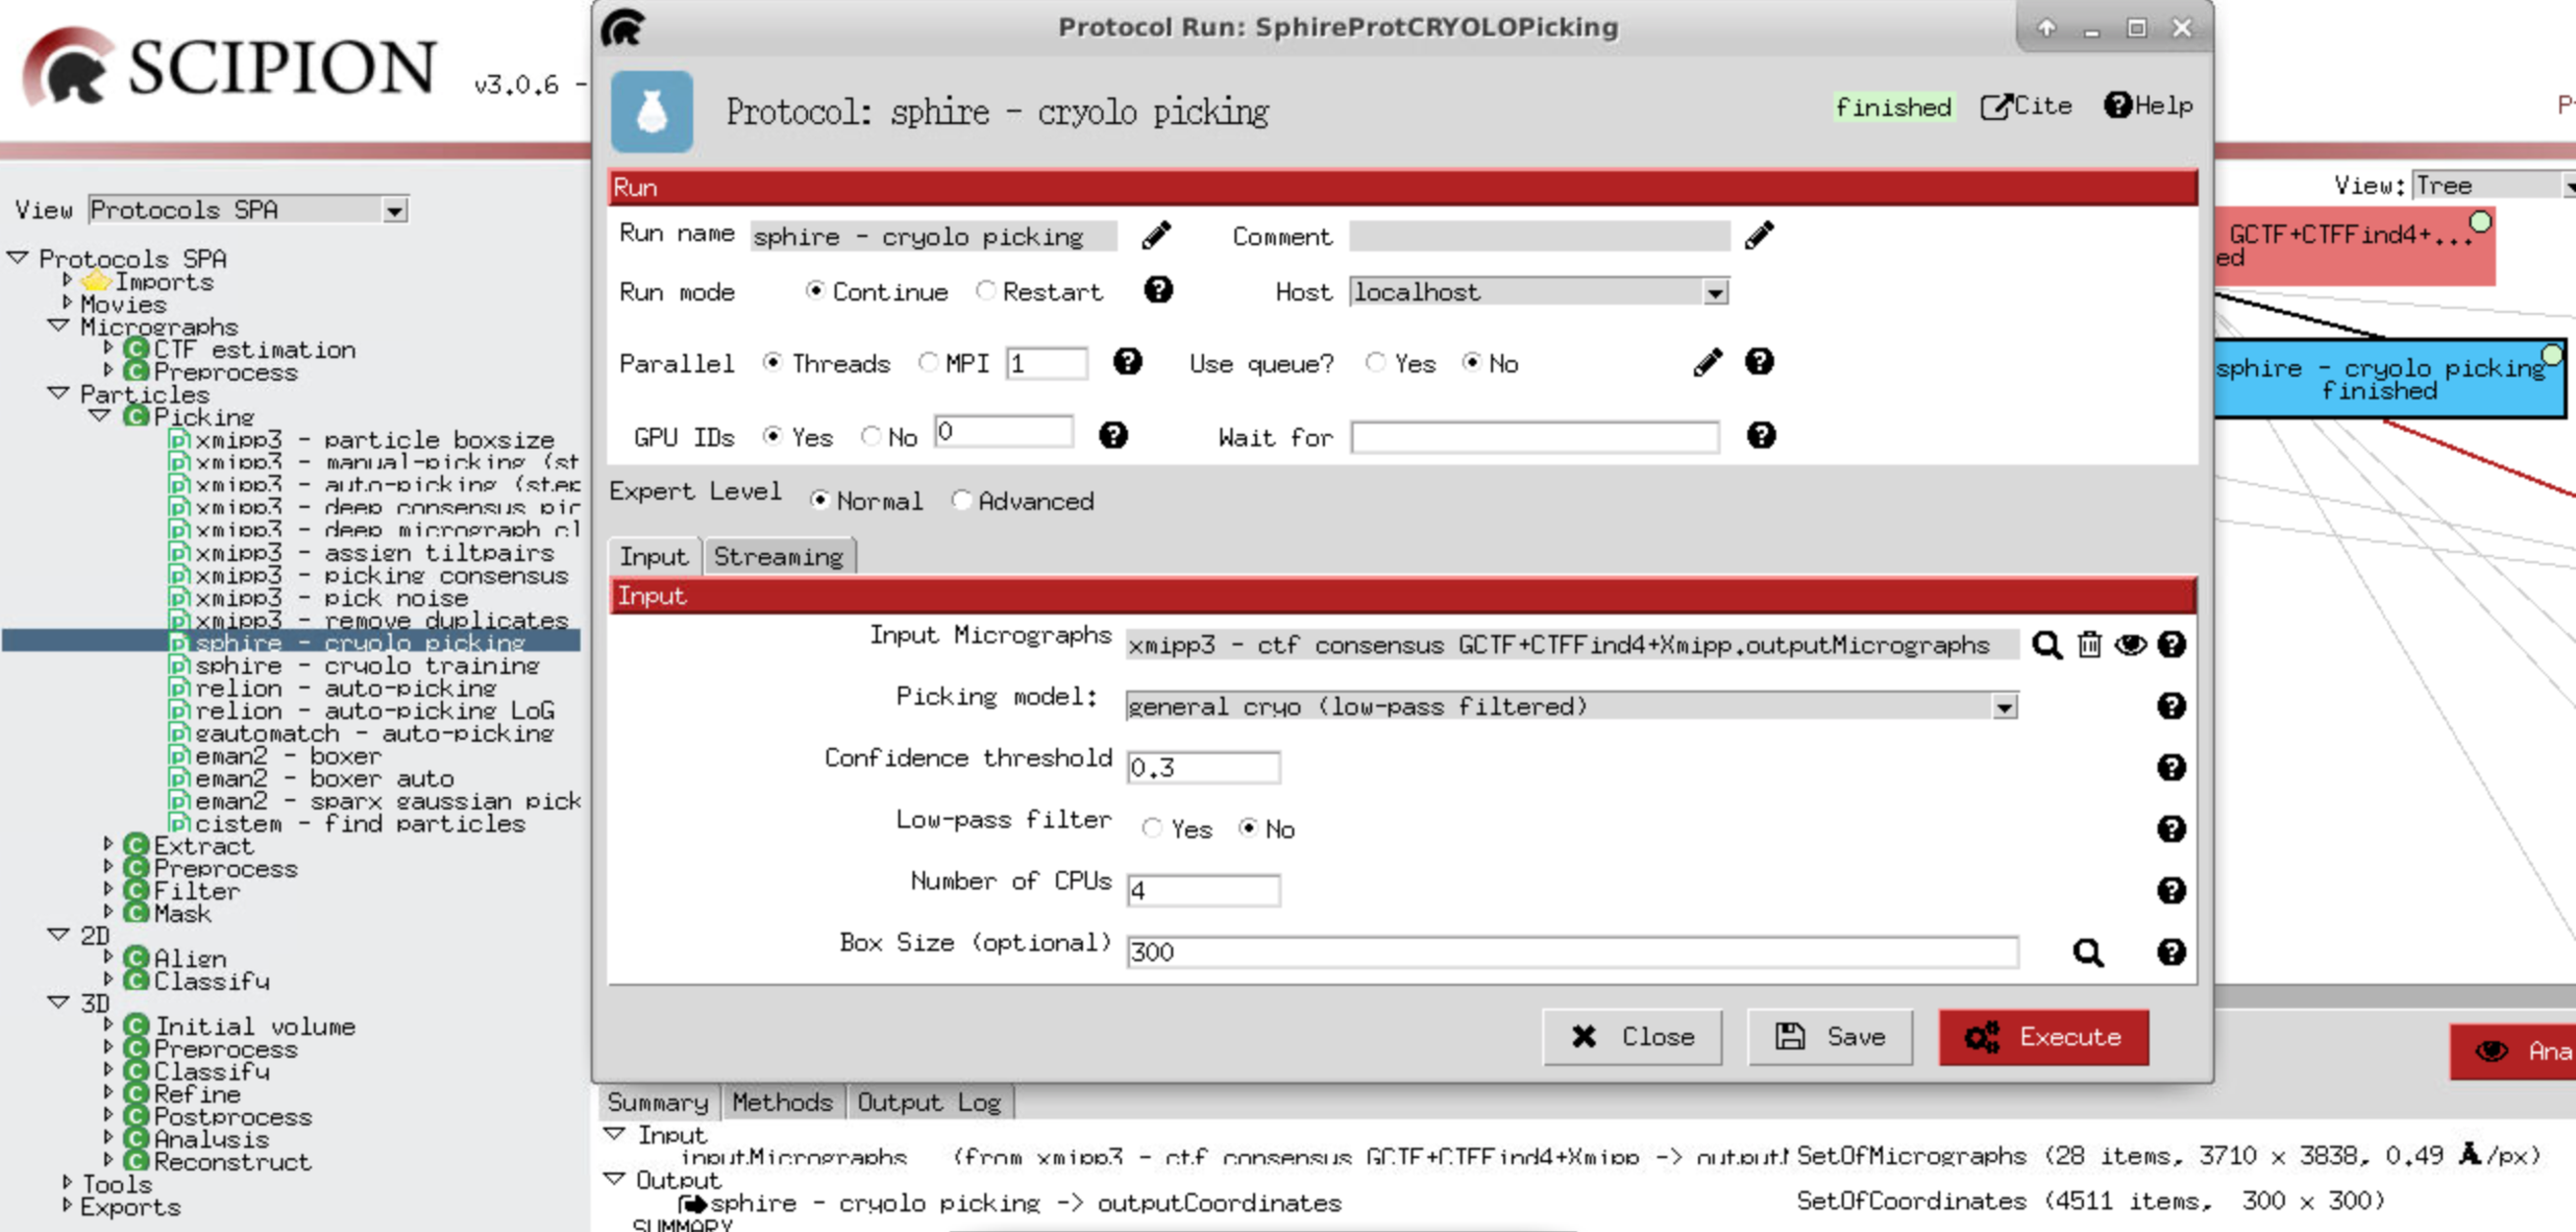
\includegraphics[width=0.95\textwidth]
  {{images/5c_sphire_CryoloPicking.pdf}}
  \caption{Completing in the protocol 3 \scommand{sphire-cryolo picking}.}
  \label{fig:sphire-cryolo}
  \end{figure}
  
The protocol \scommand{xmipp3-manual-picking (step1)} (\ffigure{fig:xmipp_manual_picking_step1}) is the first part of the \ttt{Xmipp} picking method, and allows to perform manual picking in a set of micrographs either manually or in a supervised mode. This protocol only requires as input the set of micrographs.

\begin{figure}[H]
  \centering
  \captionsetup{width=.8\linewidth} 
  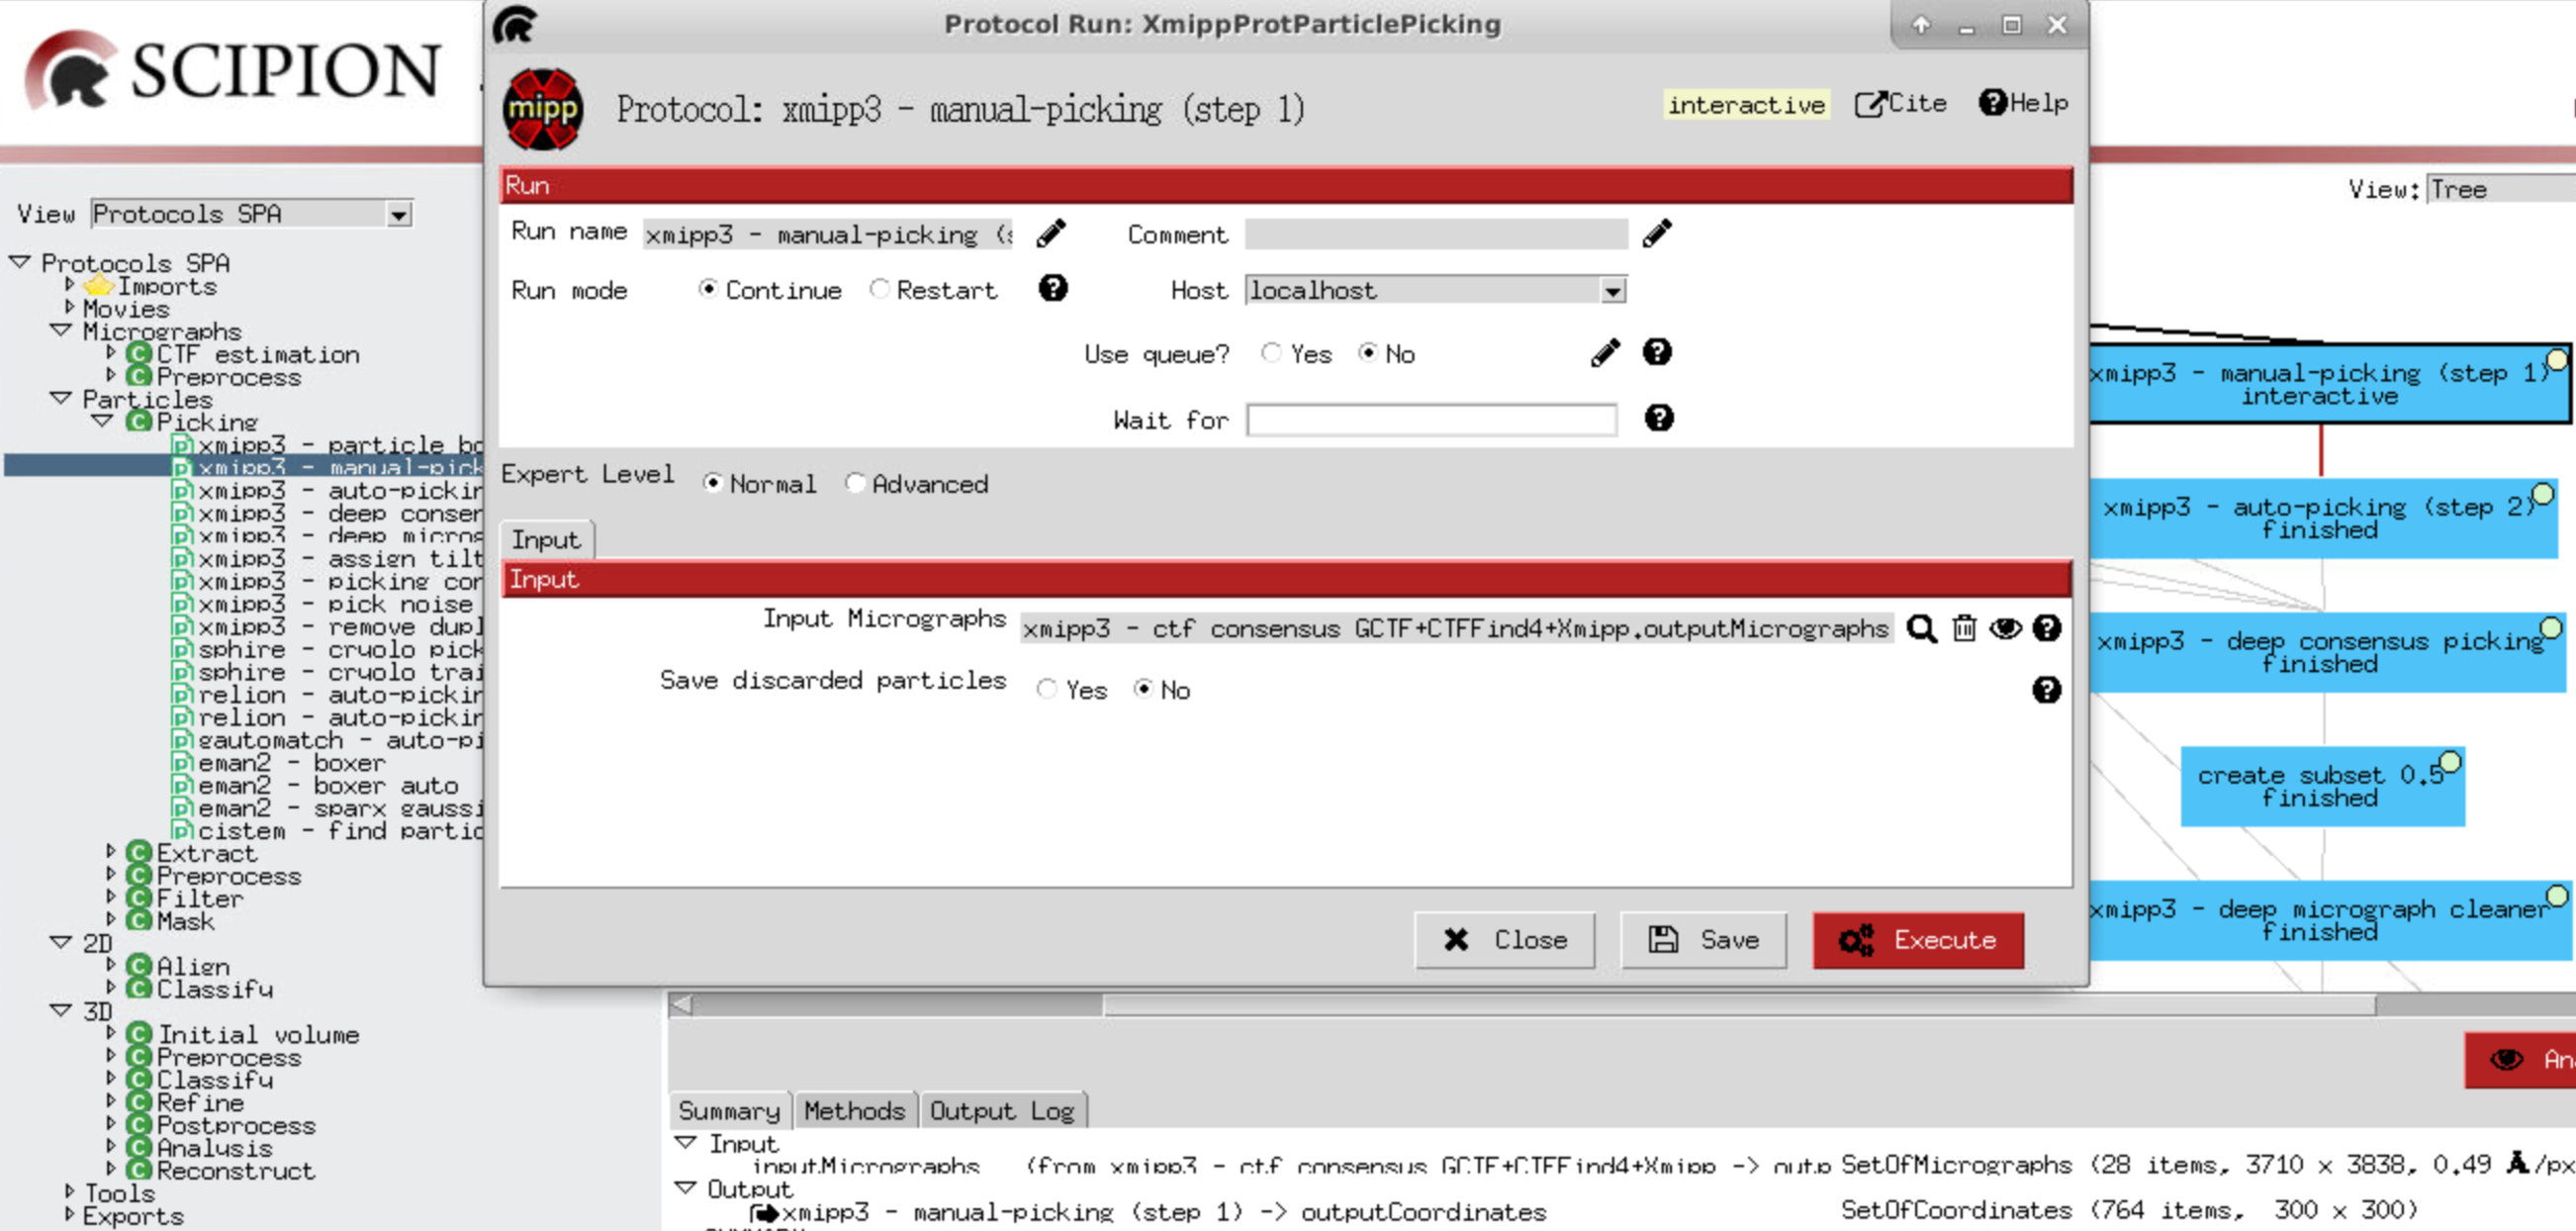
\includegraphics[width=0.95\textwidth]
  {{images/5d_xmipp3_manualPicking.pdf}}
  \caption{Filling in the protocol 4 \scommand{xmipp3- manual-picking (step1)}.}
  \label{fig:xmipp_manual_picking_step1}
  \end{figure}
  
  After executing this protocol, the respective box will become light yellow because an interactive job is running and it can be relaunched at any time.\\
  
  The \ttt{Xmipp} picking GUI contains a control panel with the list of micrographs and some other parameters. The micrograph that we are going to pick is displayed in a separate window and we can apply to it a number of filters/enhancements (like Gaussian blurring, Invert contrast, adjust histogram, etc.) just to improve the visualization of particles. Main control actions are:
  \begin{itemize}
   \item \ttt{Shift} + \ttt{Mouse wheel}: Zoom in and out of the overview window.
   \item \ttt{Mouse left} botton: Mark particles. You may move its position by clicking the left mouse button on the selected particle and dragging it to a new position.
   \item \ttt{Shift} + \ttt{Mouse left}: Remove a selected particle.
   \item You can apply filters in the micrographs to see the particles better. Select those filters in the menu \ttt{Filters}. 
  \end{itemize}

  In the manual/supervised step, we start picking manually a few micrographs (5 in this case) and then clik the \ttt{Active training} button. At this point, the program will train a classifier based on machine learning and will propose some coordinates automatically. You can ``correct'' the proposal of the classifier by adding missing particles or removing wrongly picked ones. After training with a few more micrographs, we can register the output coordinates by clicking the \ttt{Coordinates} red button.\\
  
  After manual picking, we can close the GUI and open the protocol \scommand{xmipp3- auto-picking (step 2)} (\ffigure{fig:xmipp_autopicking_step2}). Select as inputs the previous manual/supervised execution and all micrographs (\ttt{Micrographs to pick}: \ttt{Other}). The method will pick the rest of micrographs automatically. At the end, we can review the picking coordinates and we still have the chance to add/remove particles.
  
  \begin{figure}[H]
  \centering
  \captionsetup{width=.8\linewidth} 
  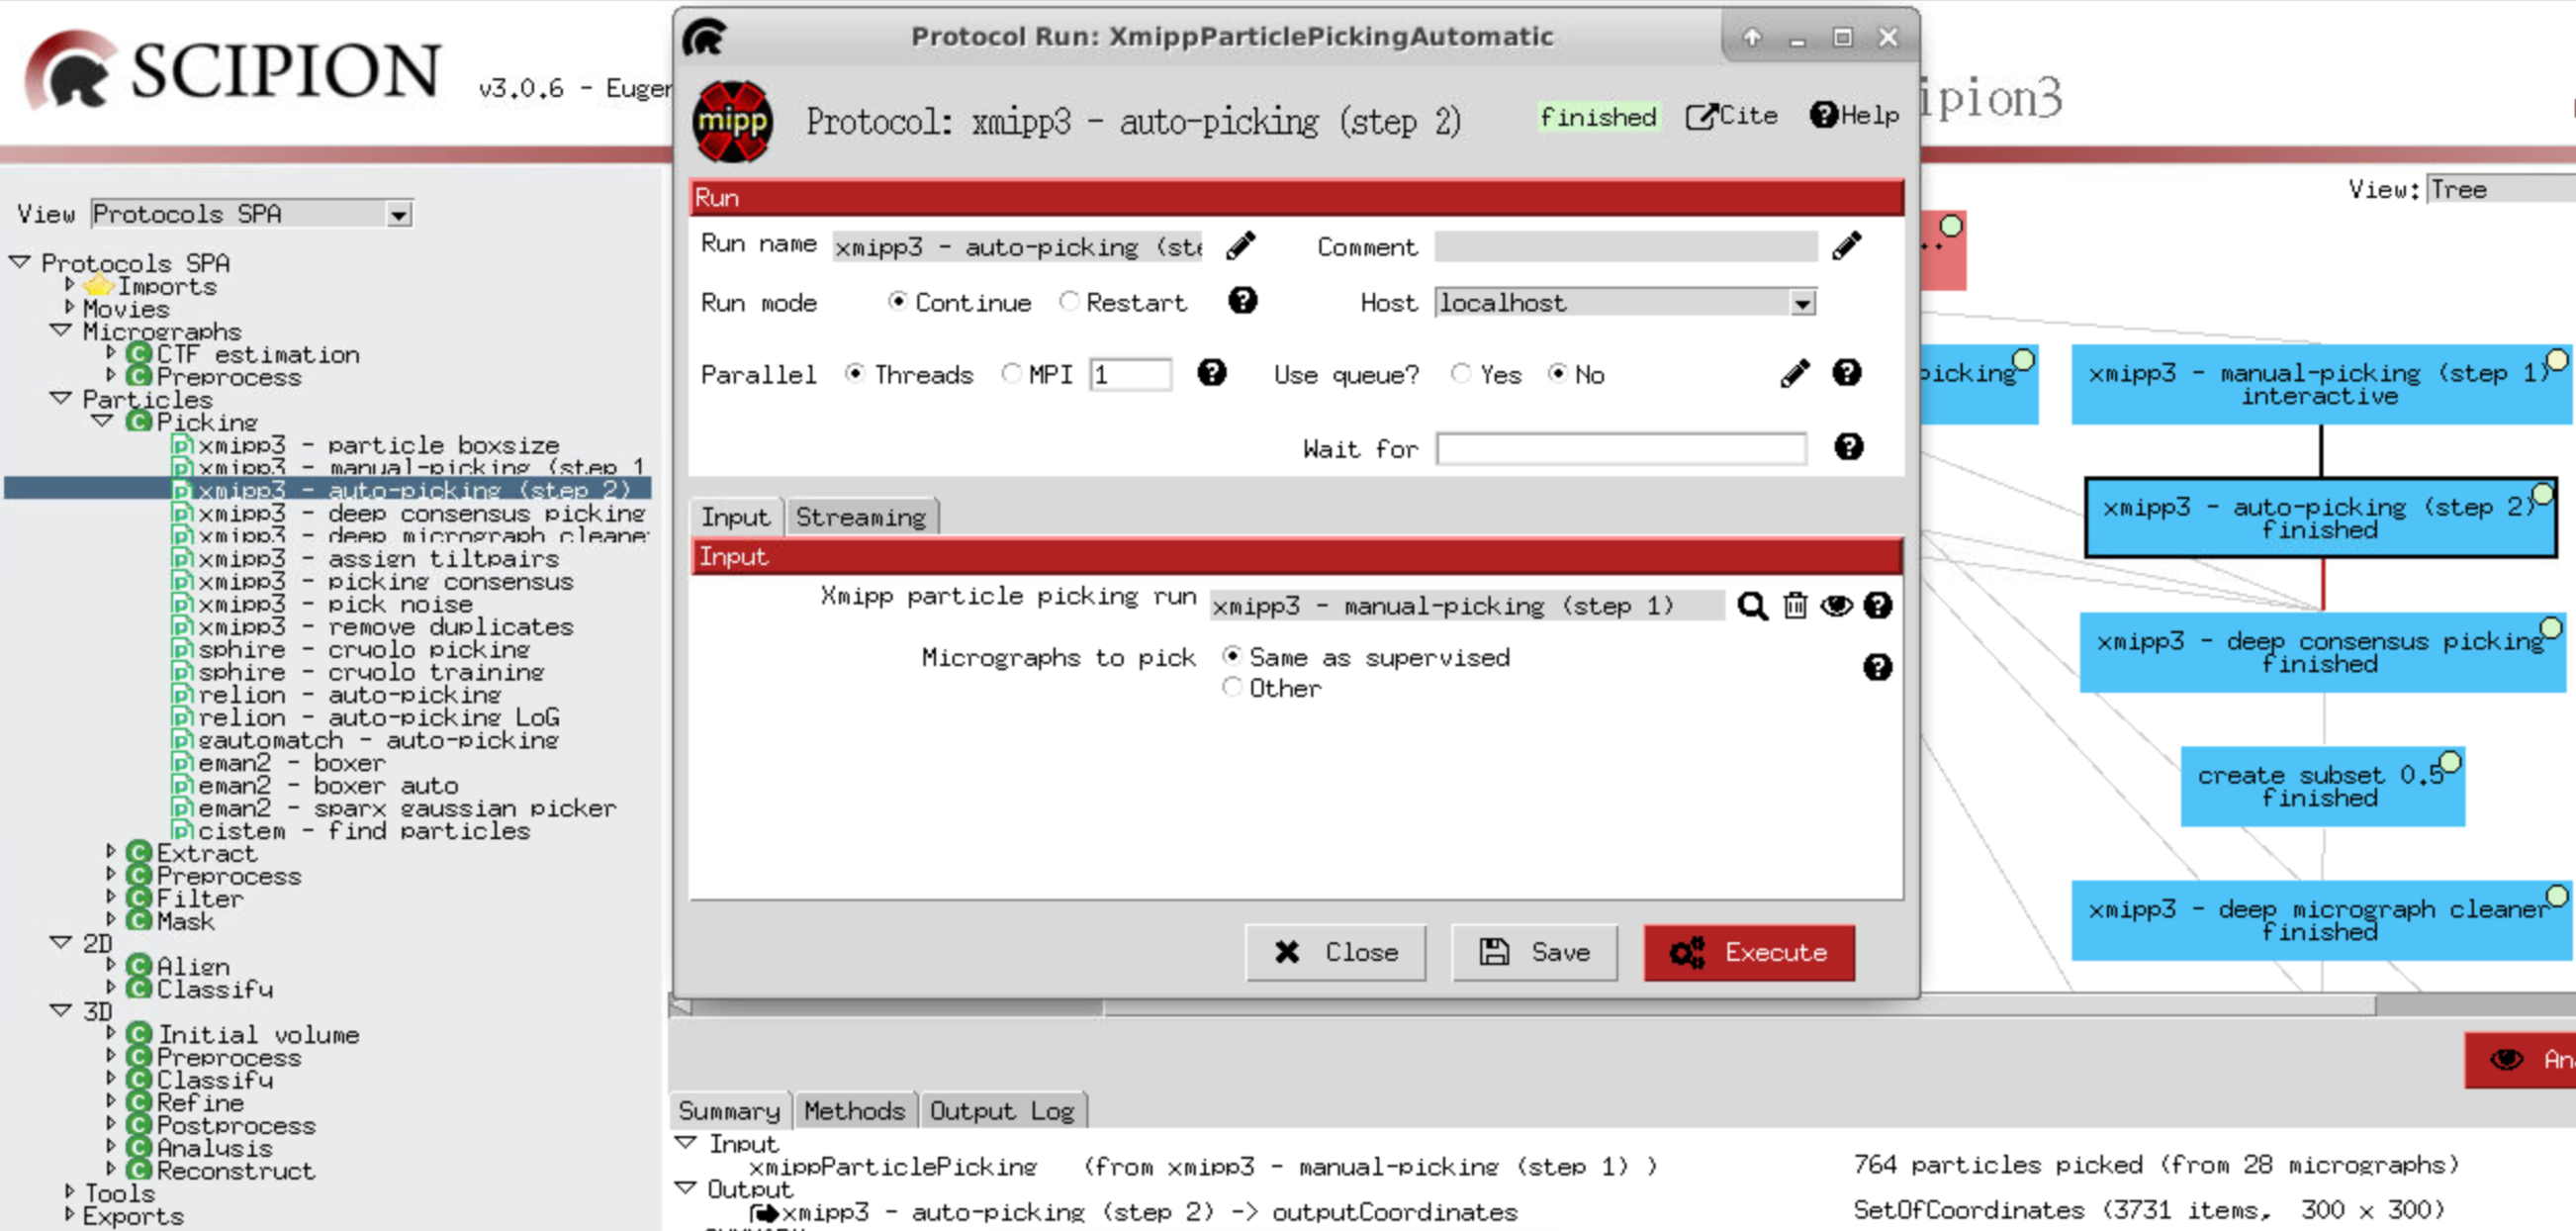
\includegraphics[width=0.95\textwidth]
  {{images/5e_xmipp3_autoPicking.pdf}}
  \caption{Completing the protocol \scommand{xmipp3-auto-picking (step 2)}.}
  \label{fig:xmipp_autopicking_step2}
  \end{figure}

  Results of all these protocols can be observed by pressing \scommand{Analyze Results}. In all cases a table details the number of particles extracted from each micrograph. Total number of particles appear in the lower part of this table, 4,291, 6,656, 4,511, 764 and 3,731 running \scommand{relion-auto-picking LoG}, \scommand{eman2-sparx gaussian picker} ,\scommand{sphire-cryolo picking}, \scommand{xmipp3-manual-picking (step1)}, and \scommand{xmipp3-auto-picking (step 2)}, respectively. As a conclusion, the three algorithms devoted to particle picking give us a similar result, around 4,500 particles. However, there are some differences among programs and we would like to keep only the coordinates of the good particles selected by the four methods.
  
  \subsection*{Consensus in particle picking}
  
  The protocol \scommand{xmipp3-deep consensus picking} (\ffigure{fig:xmipp_deep_consensus}) will try to select consensus particles among different particle picking algorithms. This protocol can also be used to get the consensus of sets of coordinates retrieved after using distinct settings of parameters with the same program. In our case, the whole sets of coordinates retrieved from the four previous methods have to be included as protocol input. 
  
  \begin{figure}[H]
  \centering
  \captionsetup{width=.8\linewidth} 
  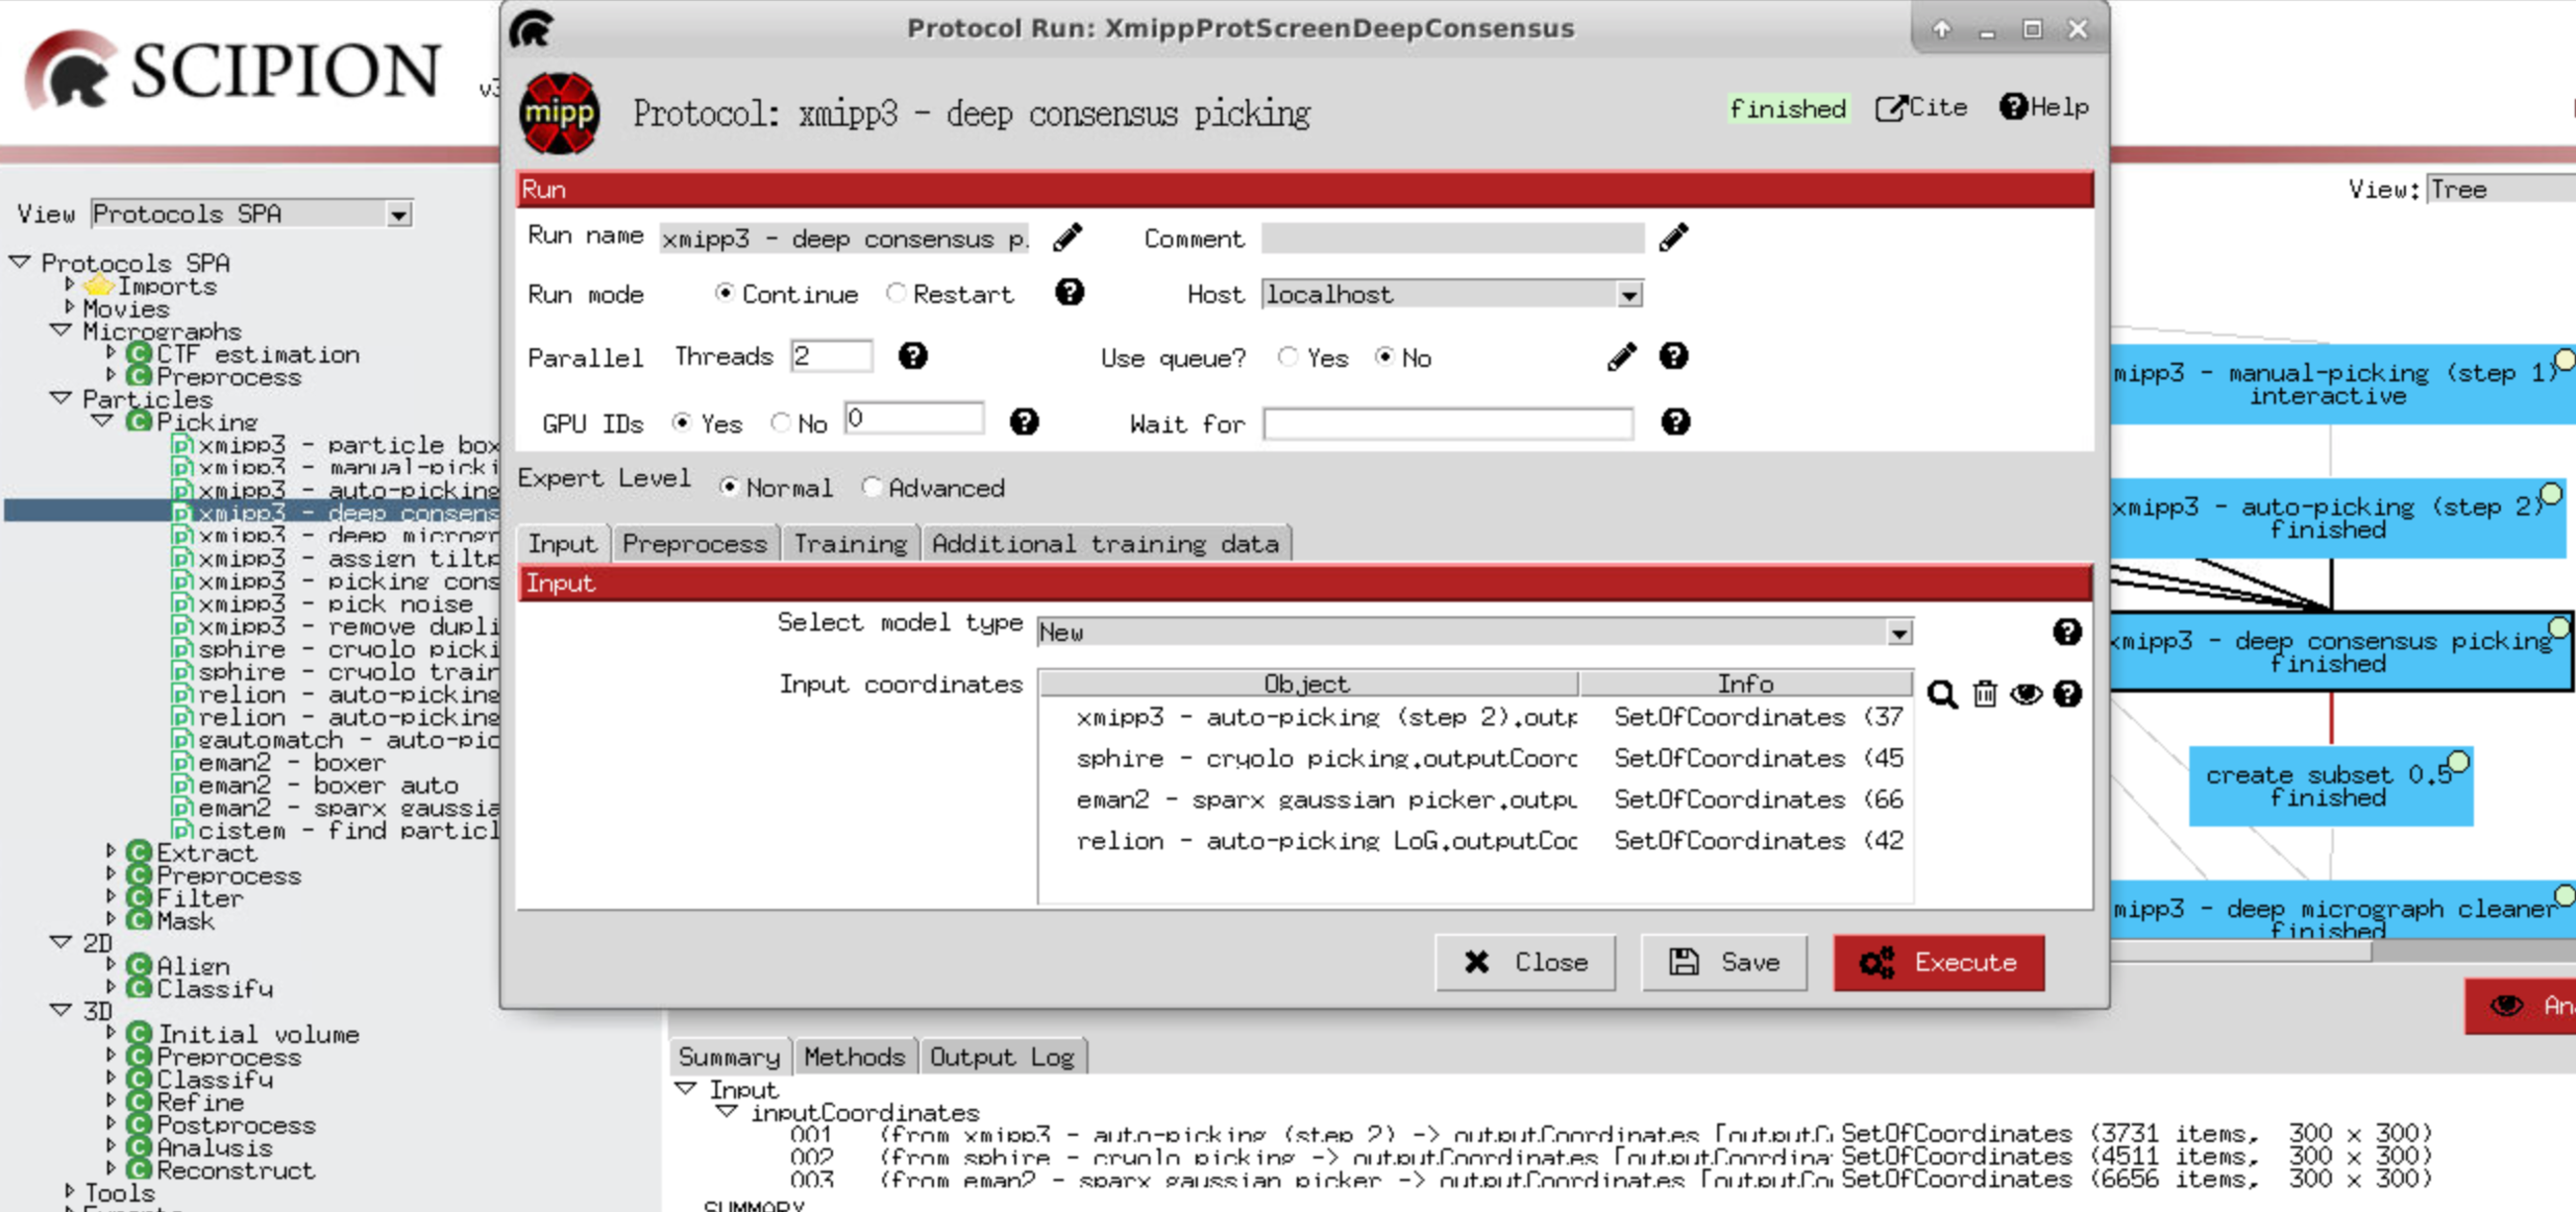
\includegraphics[width=0.95\textwidth]
  {{images/5f_xmipp3_deepConsensusPicking.pdf}}
  \caption{Completing the protocol \scommand{xmipp3-deep consensus picking.}}
  \label{fig:xmipp_deep_consensus}
  \end{figure}
  
  \ttt{(\textbf{Note}:when executed, if the process takes too long in step 13, stop the protocol and press continue.)}\\
  
  A neural network will be trained with subsets of coordinates from particles picked and not picked. Finally, the method provides a score for each particle according to the neural network predictions. After pressing \scommand{Analyze Results}, a menu allows to visualize a table showing an image and the value of the deep learning score of all the particles (\ttt{Select particles/coordinates with high 'zScoreDeepLearning1' values}). Considering that bad particles show scores values close to 0.00 and good particles scores close to 1.00, the threshold, automatically set to 0.50, allows to select good particles. In our example, from the total number of particles (4,006), 0 particles were rejected, and the total number of particles were selected to remain in the processing workflow.\\
  
  An additional cleaning step, accomplished with the protocol \scommand{xmipp3-deep micrograph cleaner}, removes particles located in carbon zones or in large impurities (\ffigure{fig:xmipp_deep_micrograph_cleaner}). Provide as input the previously selected set of coordinates and indicate the set of micrographs from which the computation will be performed. By default, we use the same as coordinates.
  
  \begin{figure}[H]
  \centering
  \captionsetup{width=.8\linewidth} 
  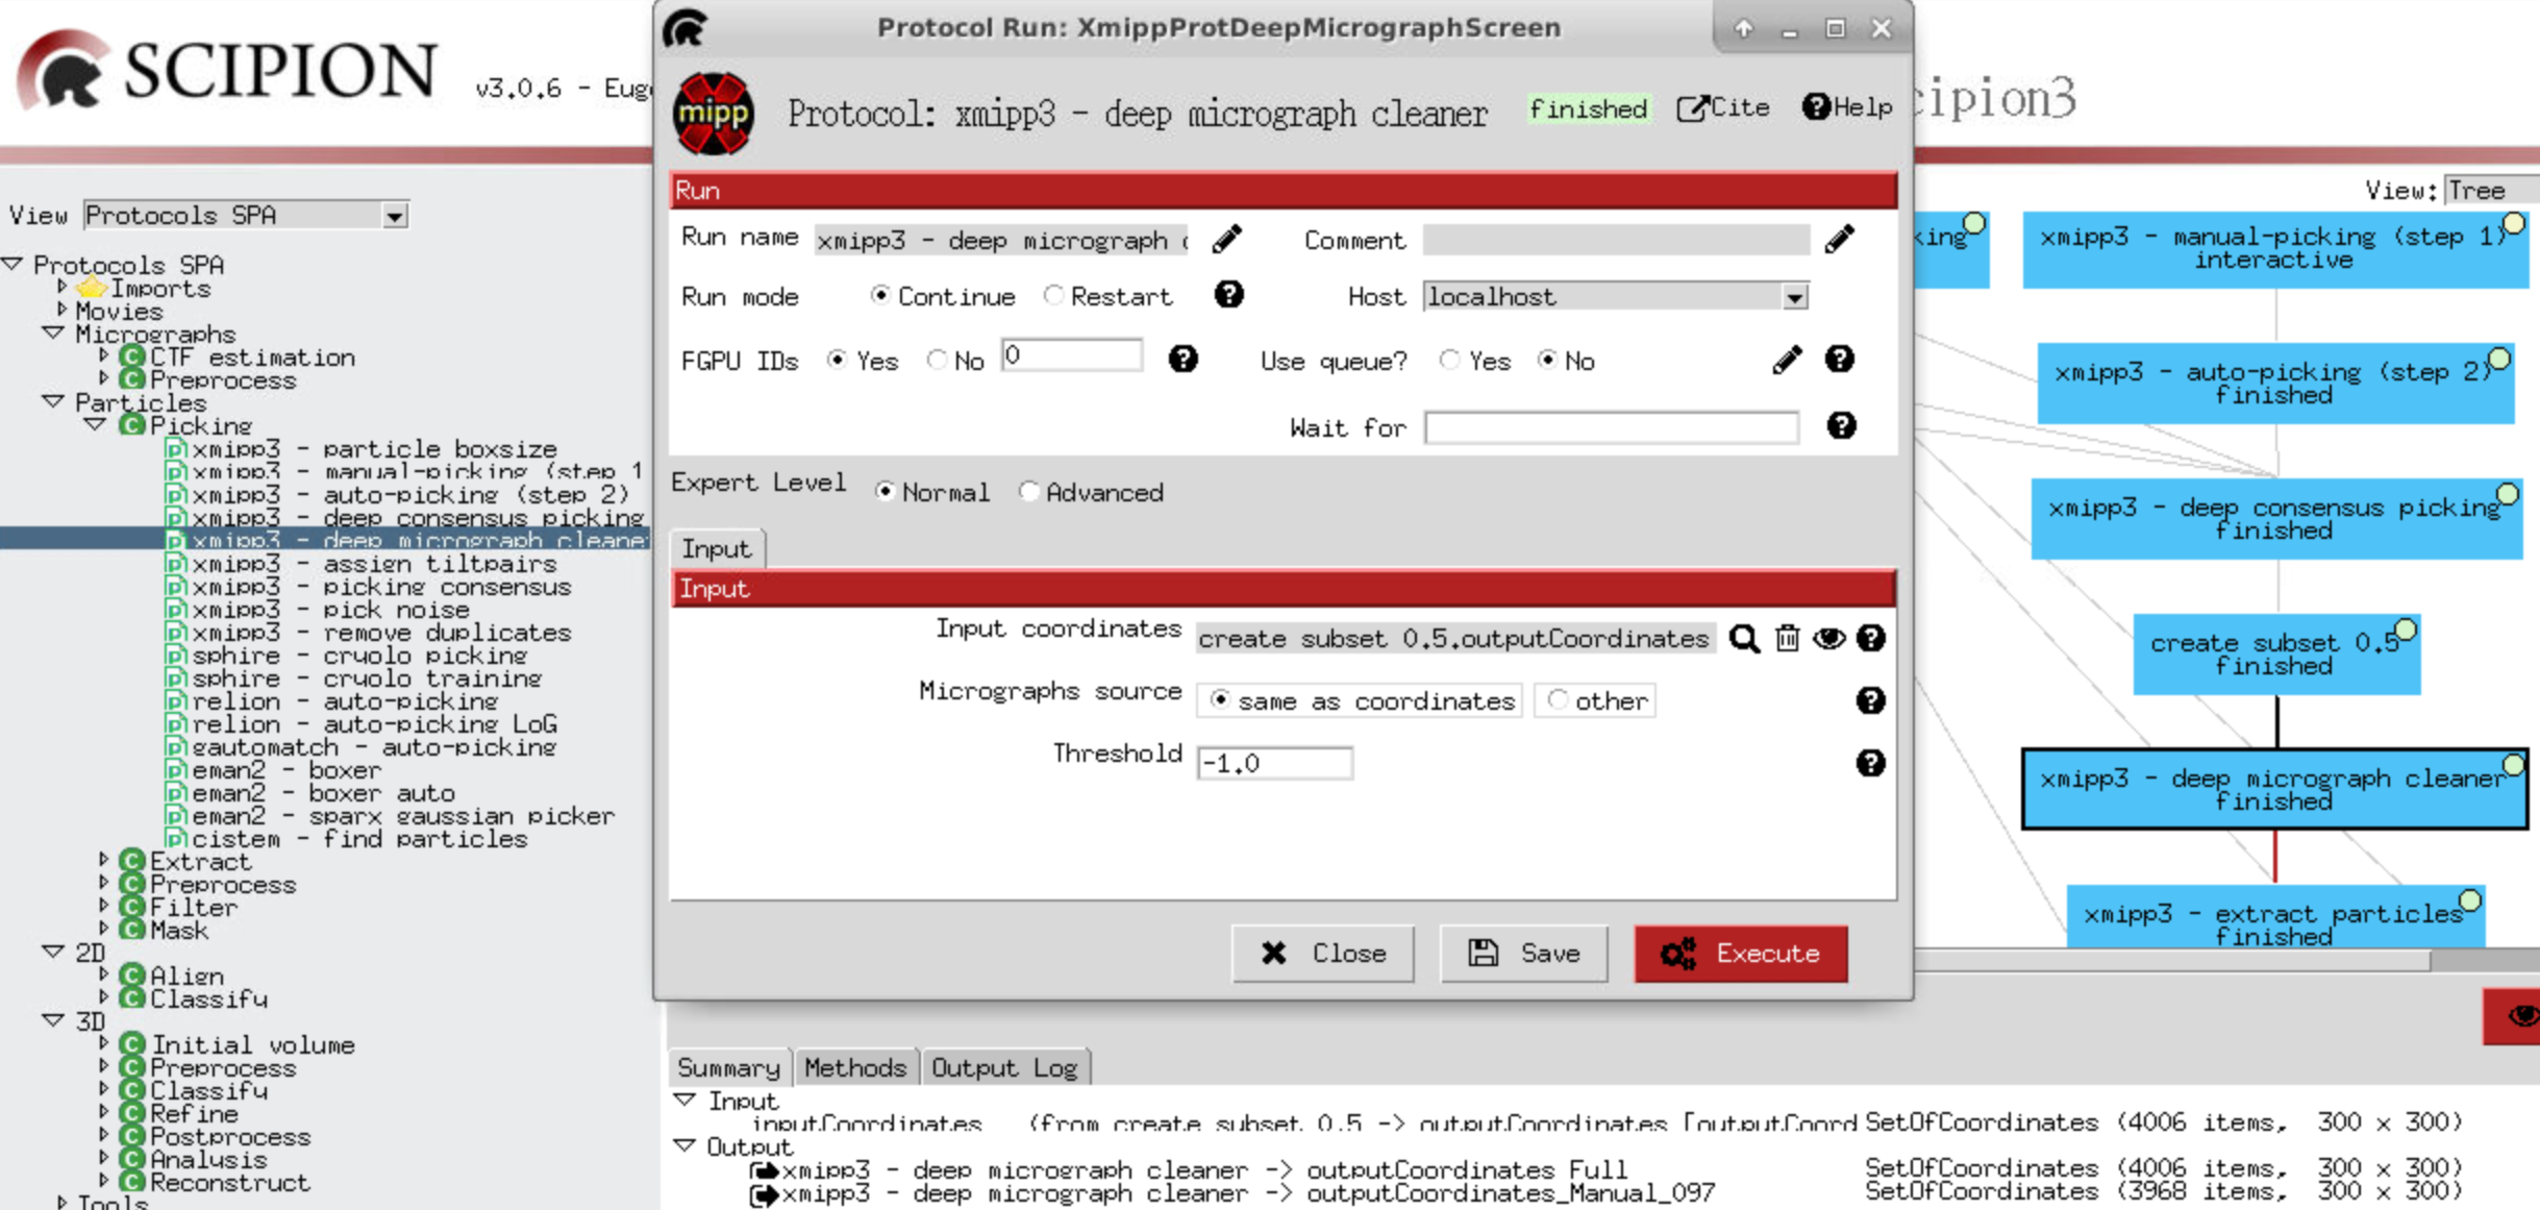
\includegraphics[width=0.95\textwidth]
  {images/5h_xmipp3_deepMicCleaner.pdf}
  \caption{Completing the protocol \scommand{xmipp3-deep consensus picking}.}
  \label{fig:xmipp_deep_micrograph_cleaner}
  \end{figure}
  
  After this additional cleaning step, 38 particles were rejected. The coordinates of the remaining reliable 3,968 particles are selected for further processing.\\ 
  
  For more information: 
\begin{itemize}
   \item \textbf{Video tutorial}:  first half of this video \url{https://www.youtube.com/watch?v=eVjQoZ8eohw&list=PLQjWIcrmtc4JjyC-_BM99_XW-VsDa4_i3&index=27}.
   \item \textbf{Theoretical lecture}: first half of this video \url{https://www.youtube.com/watch?v=yVFvN2T_soQ&list=PLQjWIcrmtc4JjyC-_BM99_XW-VsDa4_i3&index=33}.
  \end{itemize}
  

\section{Extract Particles}
 \begin{figure}[H]
  \centering
  \captionsetup{width=.8\linewidth} 
  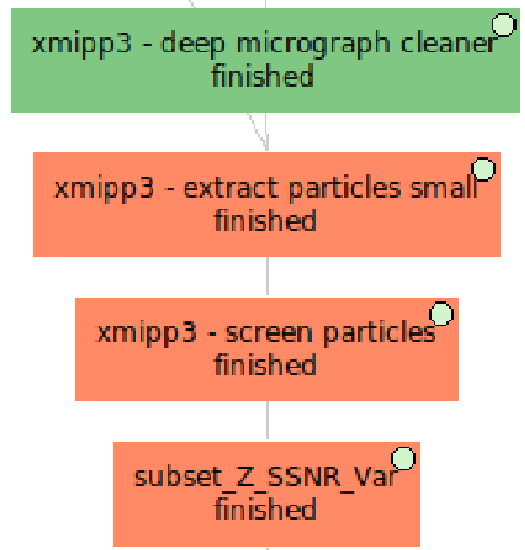
\includegraphics[width=0.35\textwidth]
  {{images/workflow_4_a.pdf}}
  \caption{Extract particles workflow (Orange color).}
  \label{fig:workflow_4_a}
  \end{figure}
Once we have a set of coordinates, we can proceed to extract particles with \ttt{Xmipp} protocol \scommand{xmipp3-extract particles} (\ffigure{fig:xmipp_extract_particles}). This protocol allows to extract, normalize and correct the CTF phases of the selected particles. As input, this protocol requires the set of coordinates and the consensus CTF values obtained in previous steps, and a downsampling factor. To save computing resources, include in the input the desired reduced size of the particles. In this particular case, 74 pixels.

\begin{figure}[H]
  \centering
  \captionsetup{width=.8\linewidth} 
  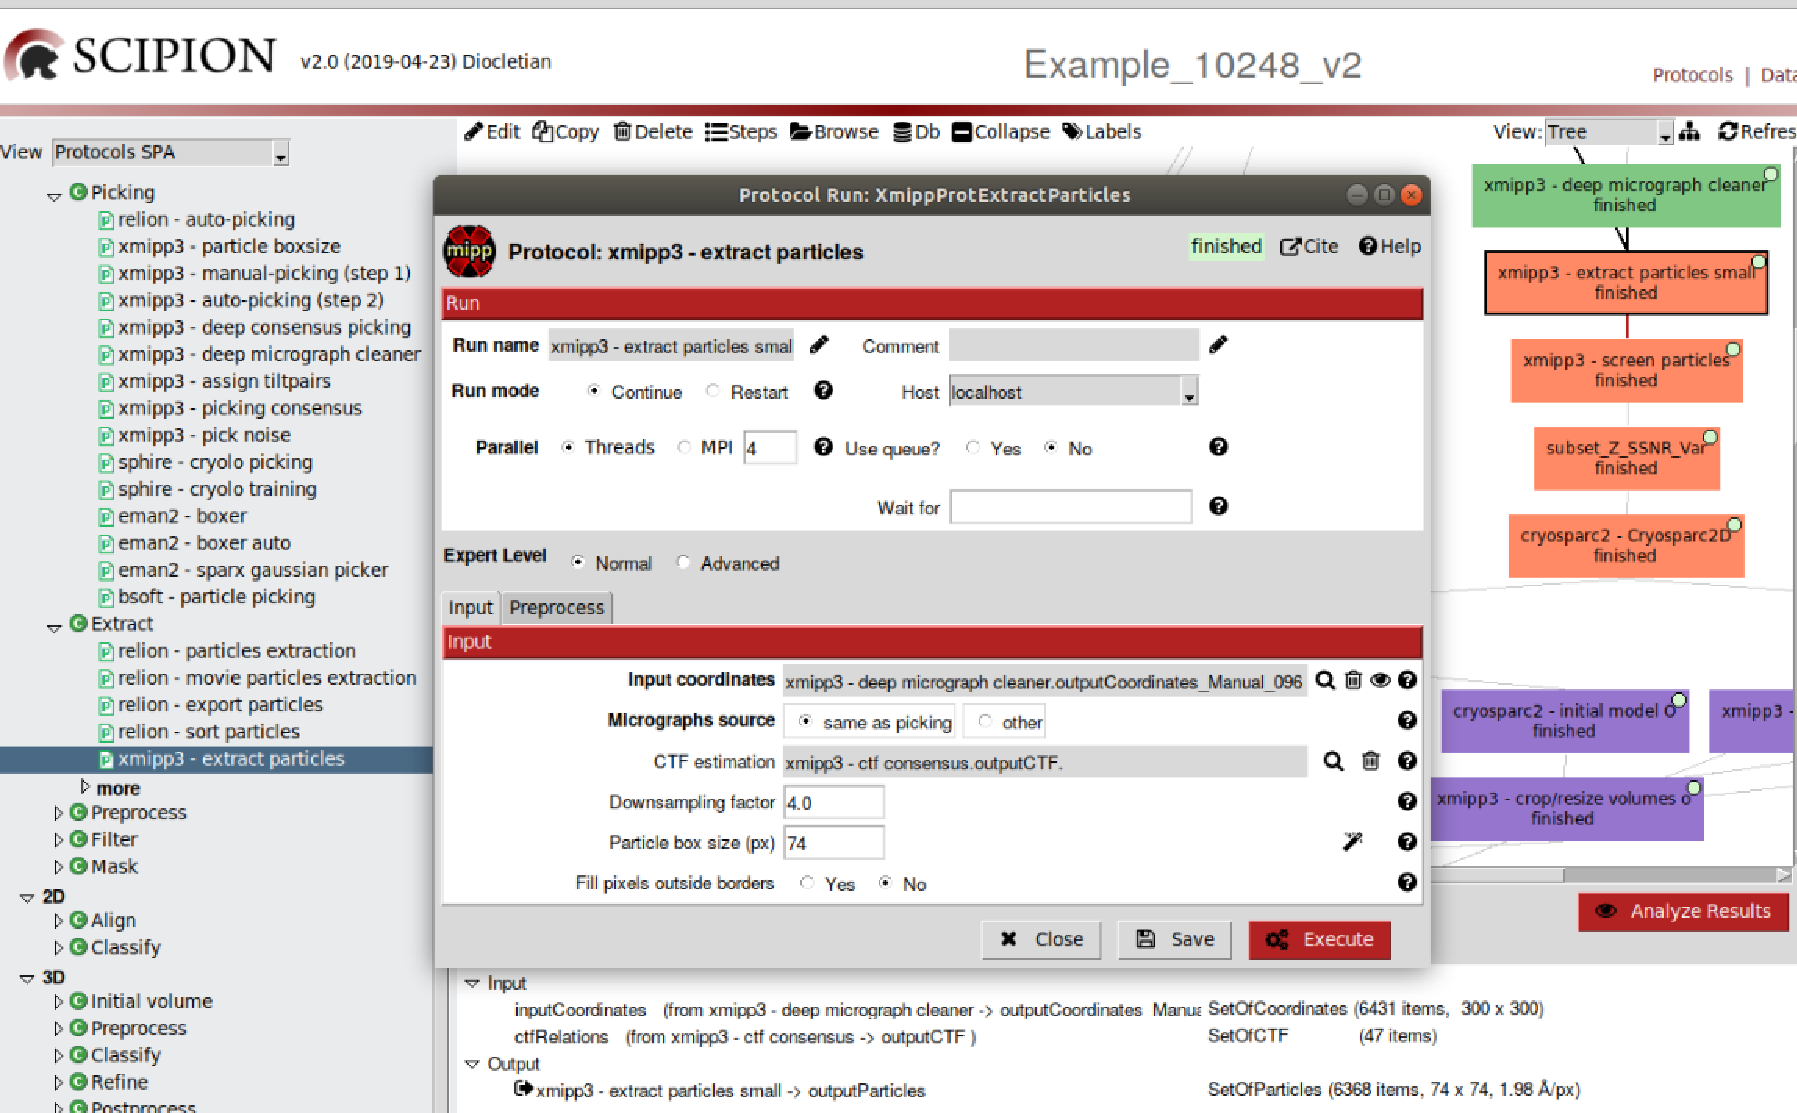
\includegraphics[width=0.95\textwidth]
  {images/xmipp_extract_particles.pdf}
  \caption{Filling in the protocol \scommand{xmipp3-extract particles}.}
  \label{fig:xmipp_extract_particles}
  \end{figure}
  
  The form tap \ttt{Preprocess} gives you additional options:
  \begin{itemize}
   \item \ttt{Invert contrast}: Option \ttt{Yes} means that bright regions become dark and the other way around.
   \item \ttt{Phase flipping}: Option \ttt{Yes} means that the protocol corrects \ttt{CTF} phases of the particles.
   \item \ttt{Normalize}: Option \ttt{Yes} (recommended) means that the particles are normalized with zero mean and one as standard deviation for background pixels.
  \end{itemize}

  As output, the protocol generates a new set of 6,368 particles after discarding other 63 particles. The extracted particles have the smaller selected size and 4 times the initial sampling rate. The images of the normalized extracted particles can be seen pressing \scommand{Analyze Results}. By default, particles displayed in gallery mode can be sorted by \ttt{Zscore}. To visualize the score associated to each particle, switch the table view by pressing the top left button. If you want to remove any of the particles showing lower score values, select them, press the mouse right button and choose \ttt{Disable}. A new subset of particles can be created by clicking on \ttt{Particles} red button. 
  
  \subsection*{Particle cleaning}
  
  Additional cleaning steps of bad particles can be performed with other screening protocols such as \scommand{xmipp3-screen particles} (\ffigure{fig:xmipp_screen_particles}). The protocol input is the subset of particles previously generated. Three different criteria for rejection can be selected, \ttt{Zscore}, \ttt{SSNR} and \ttt{Variance}. Zscore assesses the similarity of each particle with the average. SSNR evaluates the signal to noise ratio in the Fourier space. The variance is assessed for each particle in the context of particles where that particle was picked. In this particular case, we are not going to set any of the mentioned params (Zscore, SSNR and Variance). Instead, selection will be performed after visualizing the plots of those statistics. 
  
  \begin{figure}[H]
  \centering
  \captionsetup{width=.8\linewidth} 
  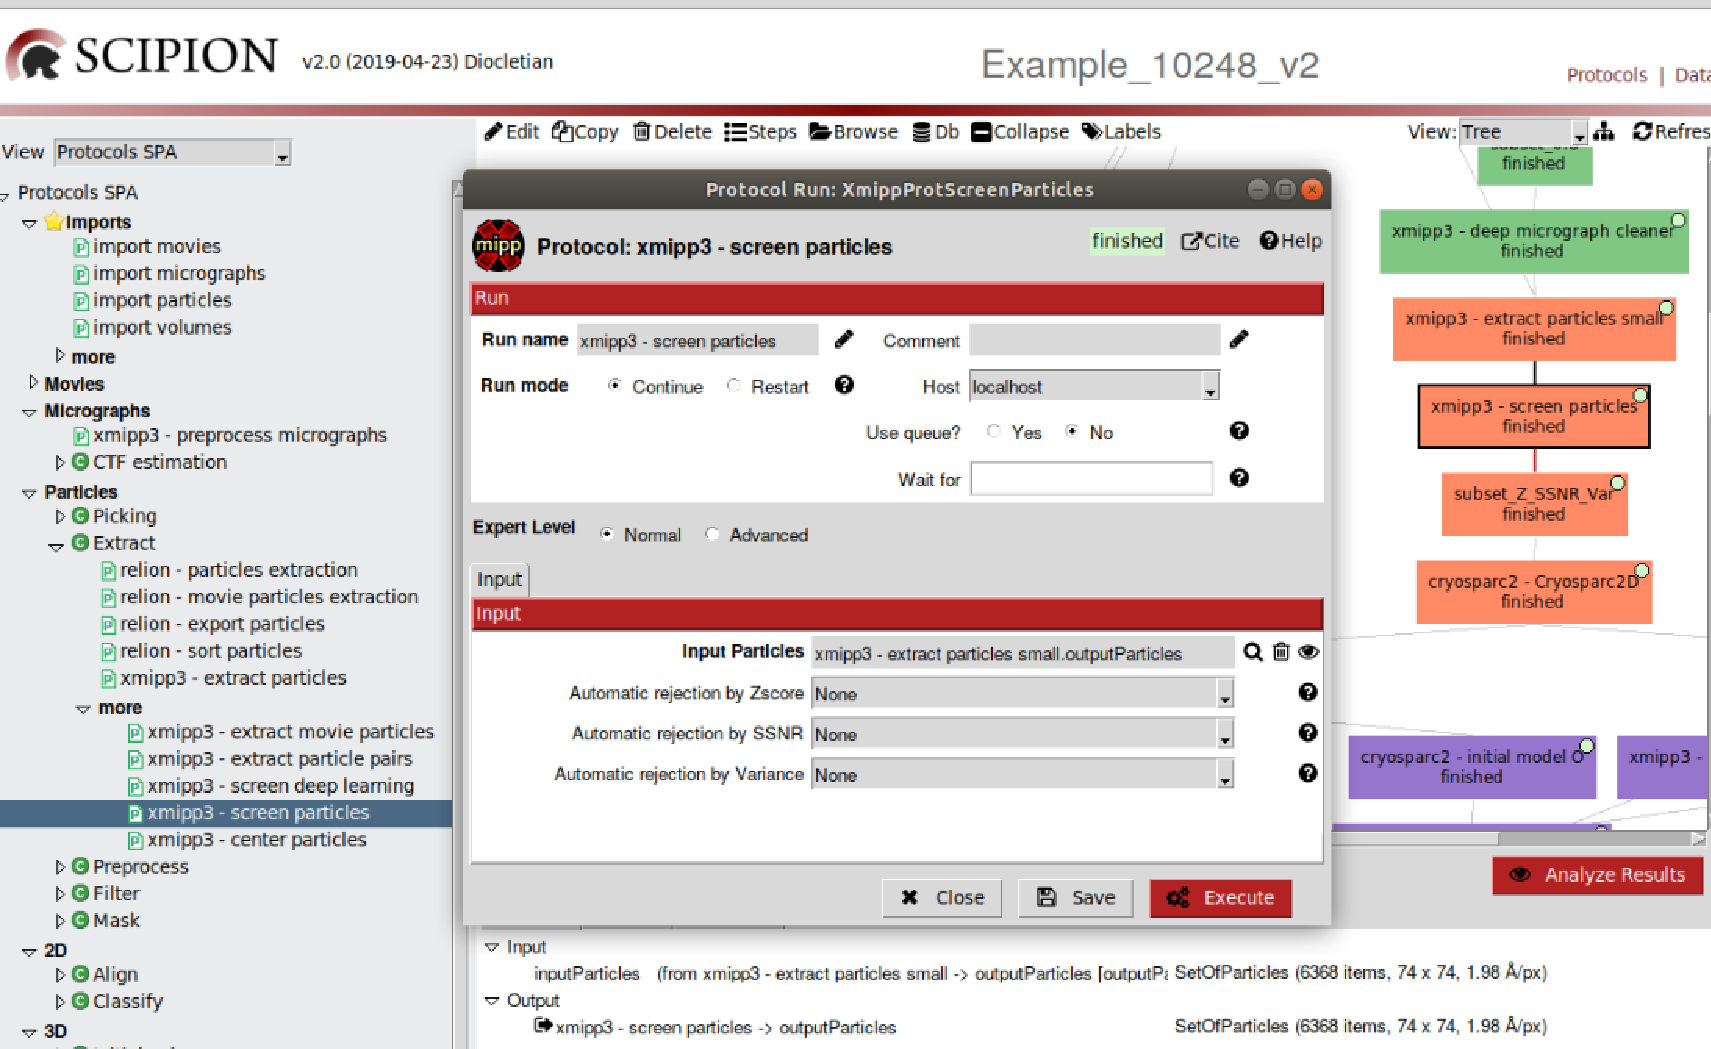
\includegraphics[width=0.95\textwidth]
  {images/xmipp_screen_particles.pdf}
  \caption{Completing the protocol \scommand{xmipp3-screen particles}.}
  \label{fig:xmipp_screen_particles}
  \end{figure}
  
  After executing the protocol without discarding any particles, we press \scommand{Analyze Results}. The plot of \ttt{Zcore} and the \ttt{Variance} histogram will be open, together with the table of particles. According to the \ttt{Zcore} plot, we discard particles with \ttt{Zcore} value higher than 3.0. According to the \ttt{Variance} histogram, we reject particles with \ttt{Variance} higher than 1.21. We can also visualize the histogram of \ttt{\_xmipp\_cumulativeSSNR}. According to this histogram, particles with \ttt{SSNR} values lower than 2.5 and higher than 5 will be discarded. The new subset of ``cleaned'' particles  obtained according those specific criteria (\ttt{subset\_Z\_SSNR\_Var}) contains 5,913 particles, after discarding 455 of them (7.1\%), that can be observed pressing \scommand{Analyze Results}. This new subset of selected particles is considered reliable for further image processing.

\section{\ttt{2D} classification}
 \begin{figure}[H]
  \centering
  \captionsetup{width=.8\linewidth} 
  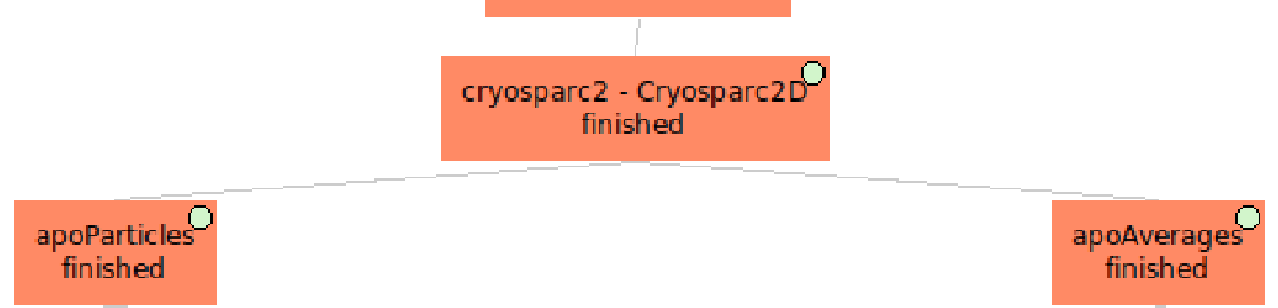
\includegraphics[width=0.95\textwidth]
  {{images/workflow_4_b.pdf}}
  \caption{\ttt{2D} classification workflow.}
  \label{fig:workflow_4_b}
  \end{figure}
The next step in image processing involves the \ttt{2D} classification of the particle images to group similar ones. This process can serve as an exploratory tool of your data and might also be used to throw away bad particles. In addition, by overlapping similar images we can obtain the average images or \ttt{2D} classes. Since these classes are the projections of the 3D object that we try to reconstruct, they can also be used in the reconstruction of the \ttt{3D} object.\\

Although there exist several \ttt{2D} classification algorithms, in this tutorial the \ttt{2D} classes will be created with the $cryoSPARC$ \citep{punjani2017cryosparc} \ttt{2D} classification method \citep{punjani2016building}, integrated in the protocol \scommand{cryosparc2- 2d classification}. We used as input the subset of particles previously selected. The \ttt{2D} classification parameters can be observed in the central tap of the protocol form in the \ffigure{fig:cryosparc2_second_tap}. Remark that we choose in advance the number of classes, 16 in this case.

\begin{figure}[H]
  \centering
  \captionsetup{width=.8\linewidth} 
  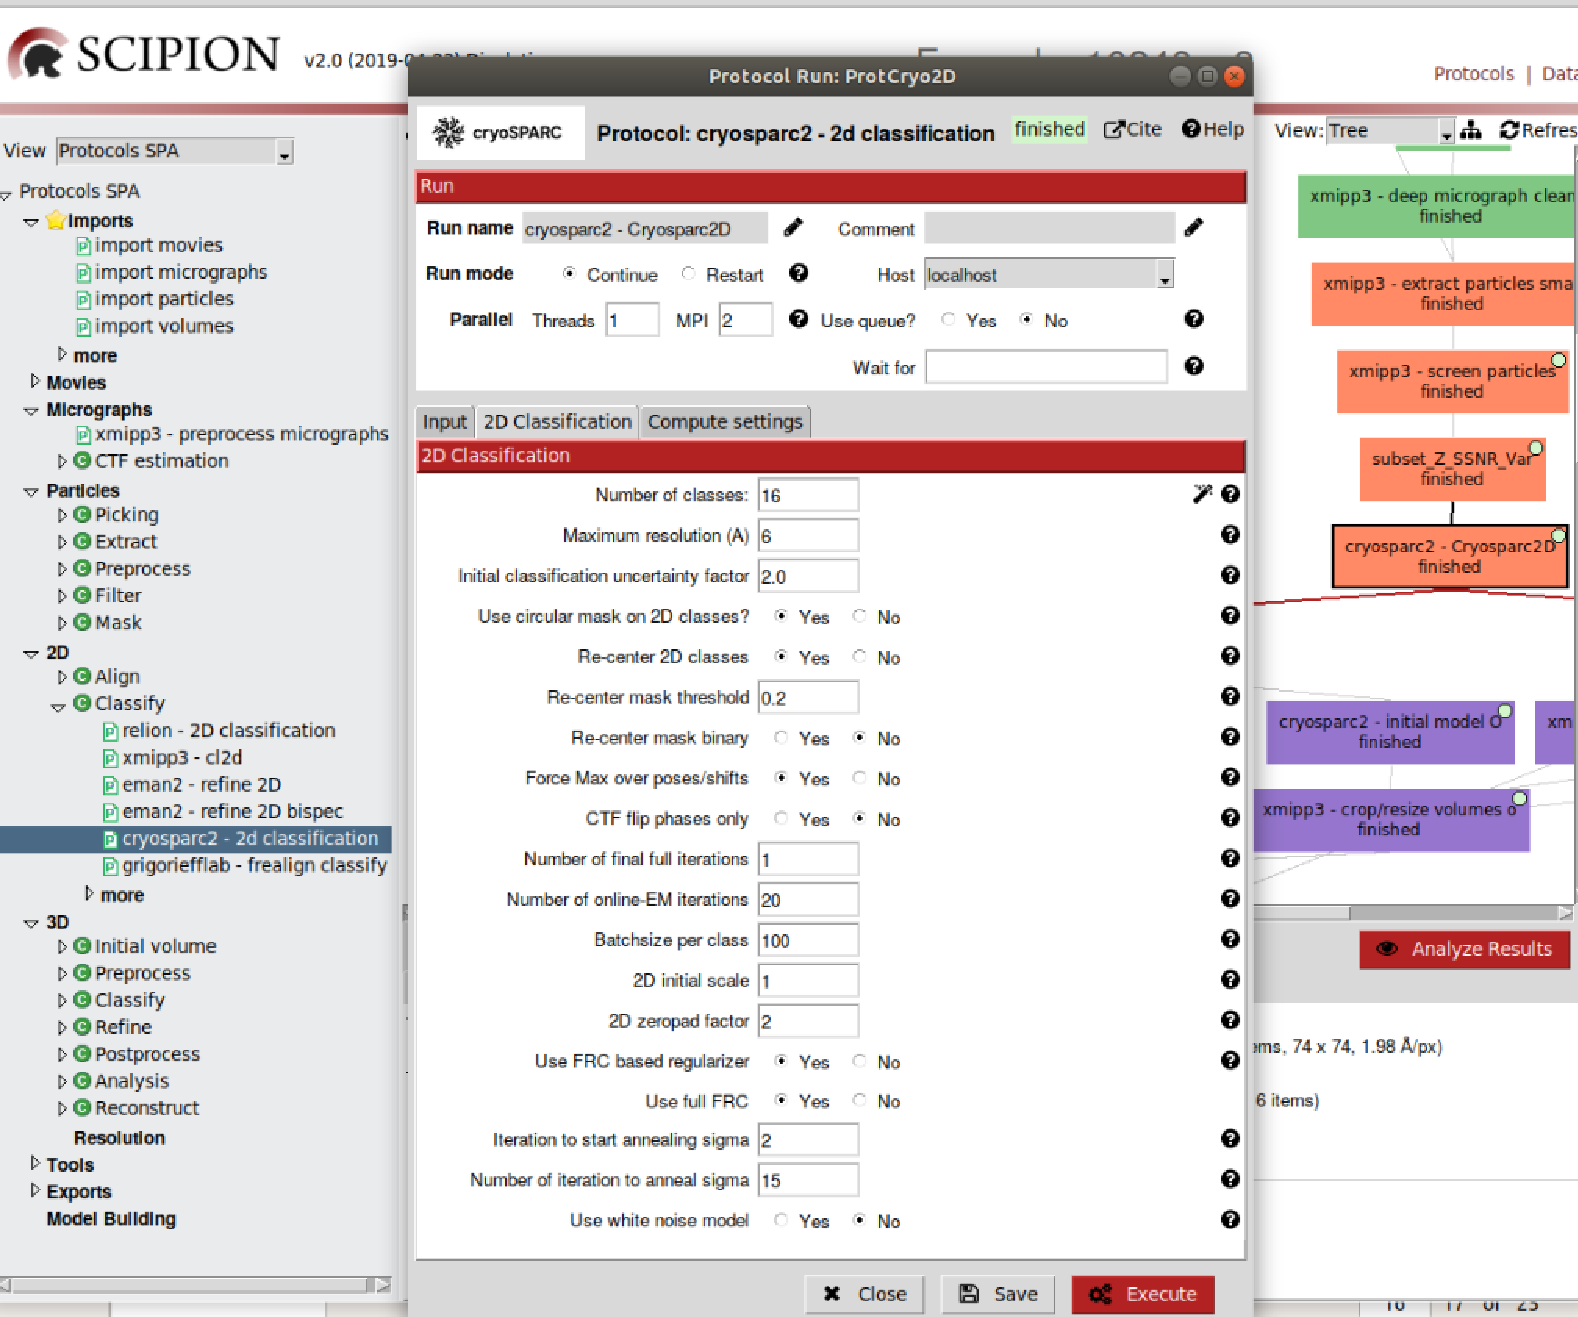
\includegraphics[width=0.95\textwidth]
  {images/cryosparc2_A.pdf}
  \caption{Filling in the second tap of the protocol \scommand{cryosparc2-2d classification}.}
  \label{fig:cryosparc2_second_tap}
  \end{figure}
  
After running the protocol, particle classes can be visualized selecting any of the two options of the menu opened with \scommand{Analyze Results}, the common \scipion viewer or the $cryoSPARC$ GUI. The final number of classes also appears in the Summary output detailed in the \ffigure{fig:cryosparc2_2branches}.

\begin{figure}[H]
  \centering
  \captionsetup{width=.8\linewidth} 
  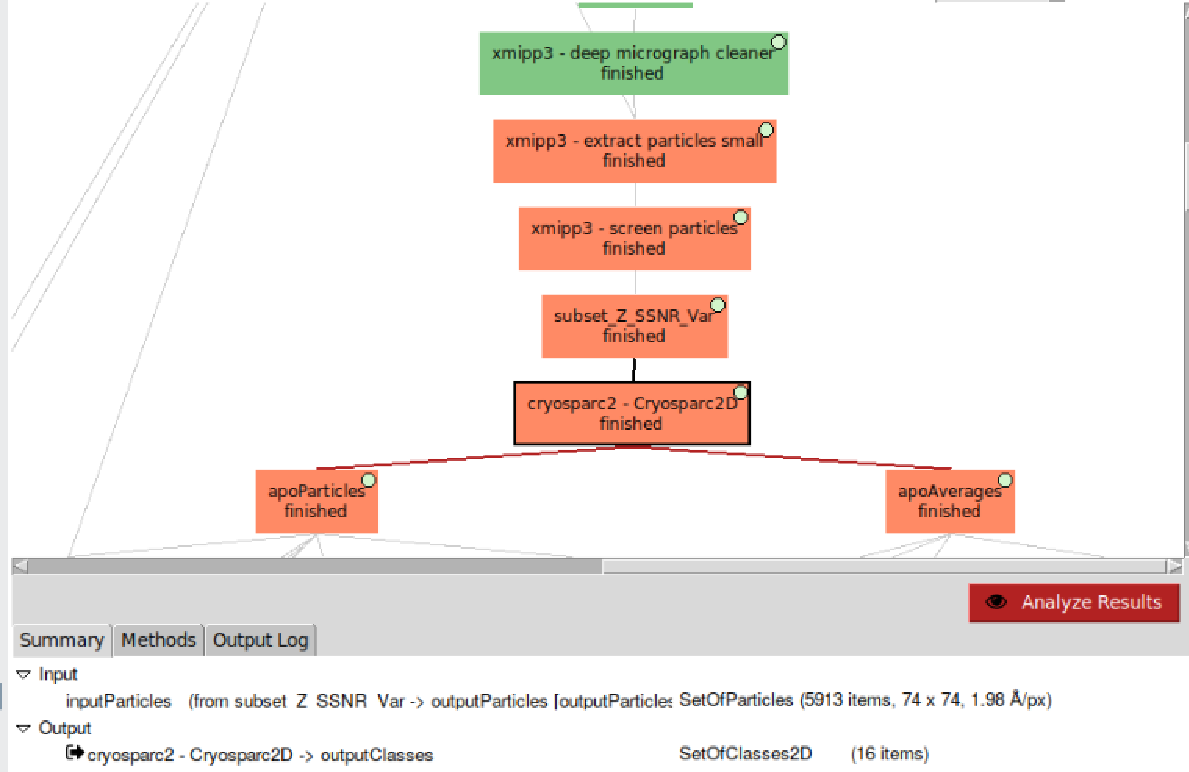
\includegraphics[width=0.95\textwidth]
  {images/cryosparc2_B.pdf}
  \caption{Summary of $cryoSPARC$ \ttt{2D classification} results.}
  \label{fig:cryosparc2_2branches}
  \end{figure}
  
Two branches derive from the \scommand{cryosparc2- 2d classification} protocol box (\ffigure{fig:cryosparc2_2branches}), pointing to two boxes, \ttt{apoParticles} and \ttt{apoAverages}, which include the whole set of particles and the \ttt{2D} classes, respectively. These two branches can be obtained by clicking in the lower part of the Summary (\ttt{cryosparc2 - Cryosparc2D -> outputClasses}). A panel will be displayed with the \ttt{2D} classes. By selecting the classes that we are interested in (14 from 16) and pressing \scommand{Particles}, a new set of 5,673 aligned particles will be created, included in the box \ttt{apoParticles} (see Summary output of the \ffigure{fig:cryosparc2_apoParticles}). 

\begin{figure}[H]
  \centering
  \captionsetup{width=.8\linewidth} 
  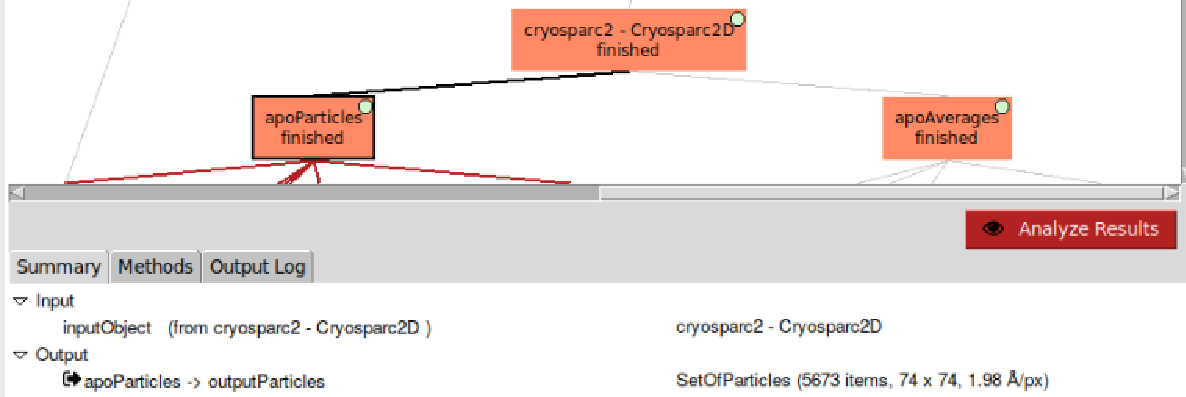
\includegraphics[width=0.95\textwidth]
  {images/cryosparc2_C.pdf}
  \caption{Summary of particle selected in \ttt{apoParticles} box.}
  \label{fig:cryosparc2_apoParticles}
  \end{figure}

If, instead, we press \scommand{Averages}, a new set of 14 class representative particles will be created, included in the box \ttt{apoAverages} (\ffigure{fig:cryosparc2_apoAverages}, Summary output). 

\begin{figure}[H]
  \centering
  \captionsetup{width=.8\linewidth} 
  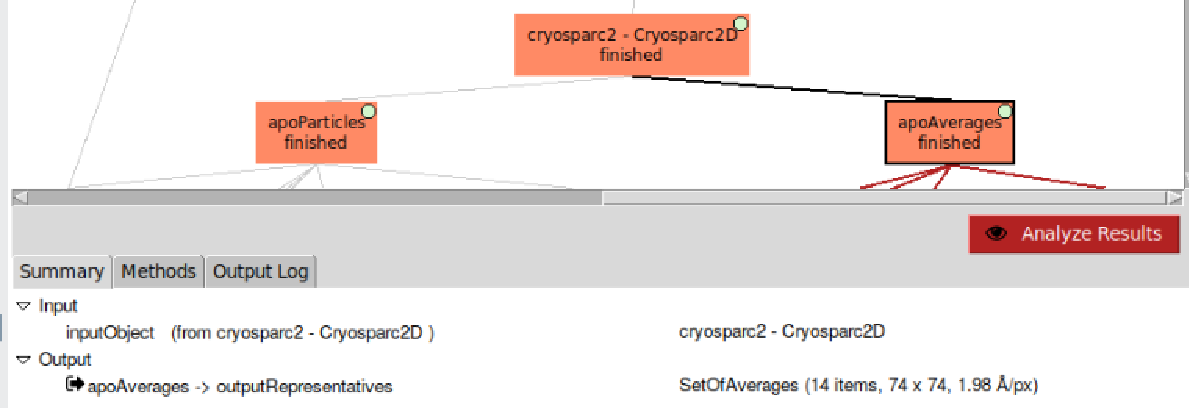
\includegraphics[width=0.95\textwidth]
  {images/cryosparc2_D.pdf}
  \caption{Summary of particle selected in \ttt{apoAverages} box.}
  \label{fig:cryosparc2_apoAverages}
  \end{figure}
  
Finally, if we press \scommand{Classes} after selecting some of the classes, a new set of classes with the number of the selected classes will be created.\\

The selected elements in the two mentioned branches, individual particles and class representative particles, will be used in the next step in the processing workflow to generate the initial volume.  

\section{Initial volume}

%%%
\section{\ttt{3D} classification and Refinement}

 \begin{figure}[H]
  \centering
  \captionsetup{width=.8\linewidth} 
  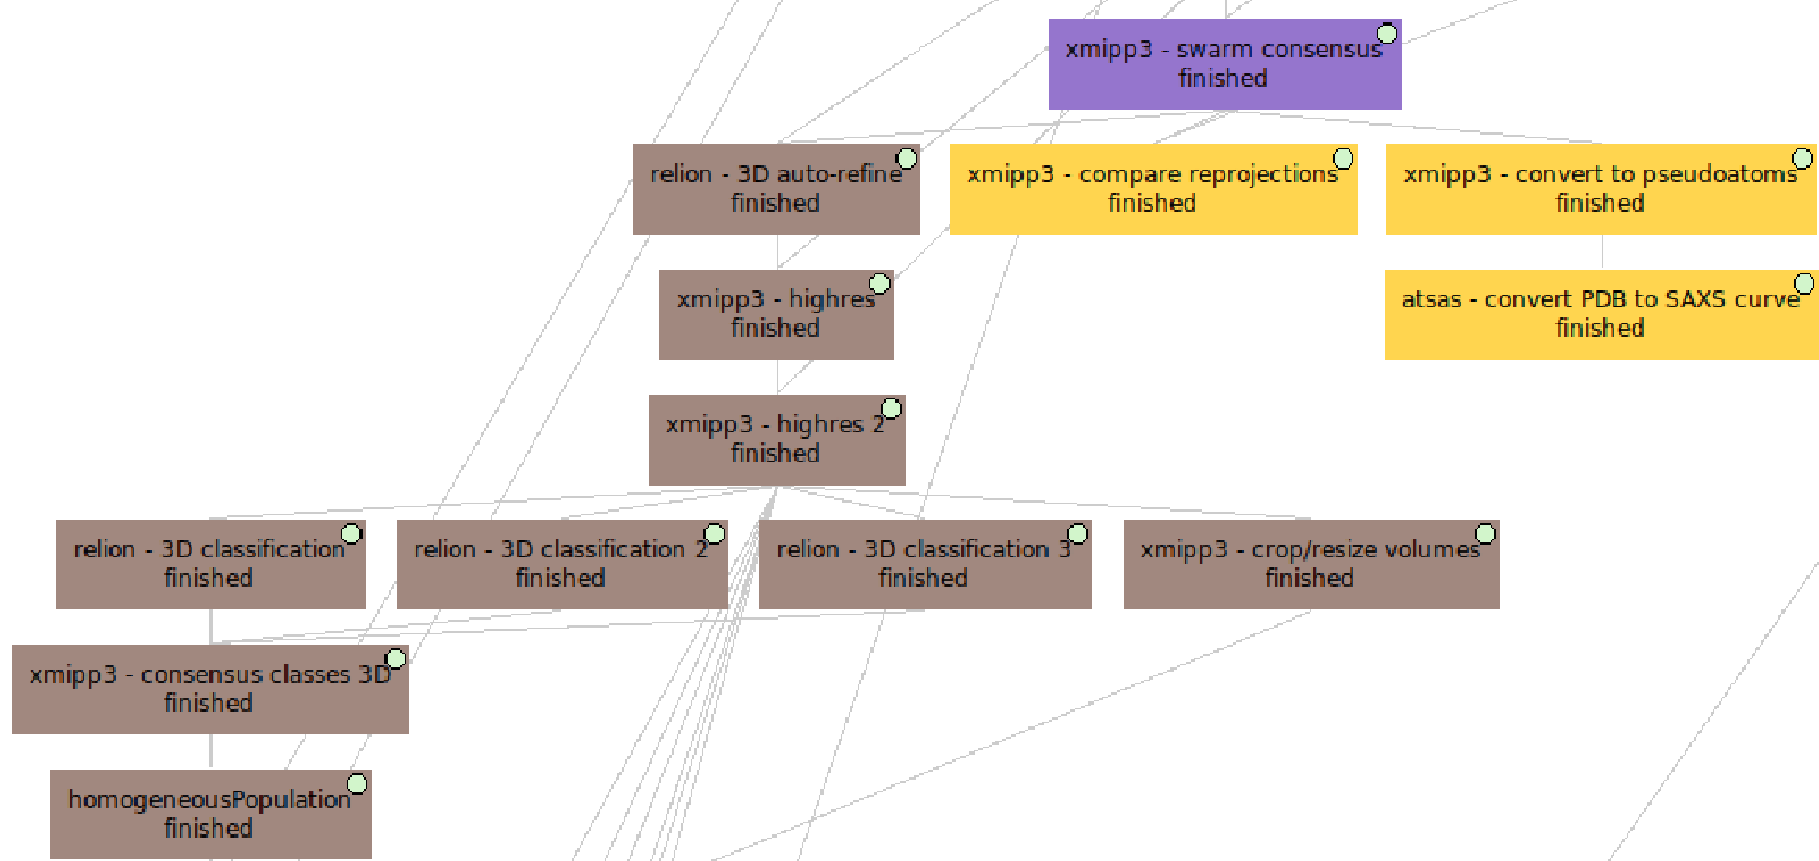
\includegraphics[width=1\textwidth]
  {{images/workflow_6.pdf}}
  \caption{Refinement and \ttt{3D} classification (Brown color).}
  \label{fig:workflow_6}
  \end{figure}

\ttt{3D} classification and Refinement are the two last overlapping steps in image processing. They consume the most time and resources with the aim of obtaining a \ttt{3D} map at the highest possible resolution. This is only feasible if data are homogeneous enough, $i.e.$, if data represent a unique conformation of the specimen.\\

Before starting with the \ttt{3D} classification properly, three consecutive steps of refinement will be performed with our initial map. The first approach to get a high resolution map in a fully automated manner was performed with the algorithm $Relion$ \ttt{auto\_refine}, based on an empirical Bayesian approach. This procedure employs the so-called gold-standard Fourier Shell Correlation (FSC) to estimate the resolution. Combined with a novel procedure to estimate the accuracy of the angular assignments, the algorithm converges. We have implemented it in the protocol \scommand{relion- \ttt{3D} auto-refine} (\ffigure{fig:initial_vol_1}). In the \ttt{Input} tap of this protocol form we include the subset of homogeneous particles  selected previously. The initial volume will be included in the \ttt{Reference 3D map} tap, as well as a \ttt{Initial low pass-filter (A)} of 60.0. This tap gives you the possibility of using \ttt{Reference mask (optional)} and, in some cases, $e.g$ non-empty icosahedral viruses, a \ttt{Second reference mask (optional)}.

\begin{figure}[H]
  \centering
  \captionsetup{width=.8\linewidth} 
  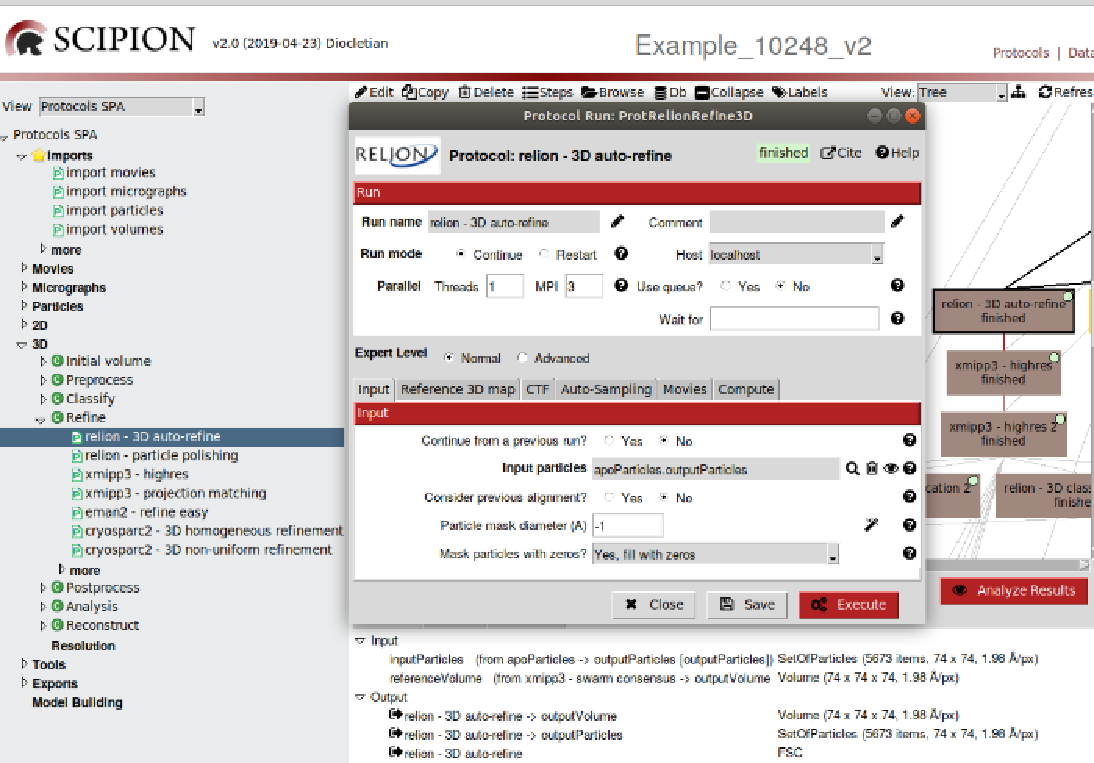
\includegraphics[width=0.95\textwidth]
  {{images/relion_3D_auto_refine_1.pdf}}
  \caption{Completing the params of the protocol \scommand{relion- \ttt{3D} auto-refine}.}
  \label{fig:relion_3D_auto_refine_1}
  \end{figure}

There are three questions in the tab \ttt{CTF}: 
\begin{itemize}
 \item \ttt{Do CTF correction?}, set to \ttt{Yes} to perform full phase + amplitude CTF correction.
 \item \ttt{Has reference been CTF-corrected?}, set to \ttt{No} because the Fourier transforms of the reference projections are not multiplied by the \ttt{CTF} in the first iteration. 
 \item \ttt{Do manual grouping ctfs?}, set to \ttt{No} because we have enough number of particles that we do not need to group them.
\end{itemize}

The \ttt{Angular sampling interval (deg)} option in the tab \ttt{Auto-Sampling} will be used only in the first few iterations. Later the algorithm will automatically increase its value until convergence. For symmetries lower than octahedral or icosahedral we use the default values of \ttt{Angular sampling interval (deg)} and \ttt{Local search from auto-sampling (deg)}.\\

\ttt{Movies} tab allows to align movie-particles of each frame and execute later a protocol of particle polishing.\\

After executing 7 iterations a refined map of 5.05 \AA\ of final resolution was obtained as output, with the same size and sampling rate that we had in the inputs. Press \scommand{Analyze Results} and visualize any iteration or the last one by default. Concerning particles, their angular assignment and the \ttt{\*\_optimiser.star file}, with general information about the refinement process, can be shown. Different volumes can be \ttt{2D} or \ttt{3D} visualized, such as each half map, both, or the final one. \ttt{SSRN} and resolution \ttt{FSC} plots are also available.\\

The next two following steps of refinement have been performed with the $Xmipp$ algorithm \ttt{highres} \citep{sorzano2018new} that we have implemented in the protocol \scommand{xmipp3-highres} (\ffigure{fig:xmipp_highres_1}). This method computes a weight for each particle and performs both global and local alignment. Iterations can be performed one by one, removing particles that worse fit the map from one iteration to the next one. This \ttt{3D} refinement protocol uses as input the refined map obtained from $Relion$ \ttt{auto\_refine} and the same set of particles used by this algorithm. The \ttt{Symmetry group} has been also included in the \ttt{Input} tap. In the \ttt{Angular assignment} tap we choose \ttt{Global} as \ttt{Image alignment} and 1 \ttt{Number of iterations} with 4 \AA\ as \ttt{Max. Target Resolution}.

\begin{figure}[H]
  \centering
  \captionsetup{width=.8\linewidth} 
  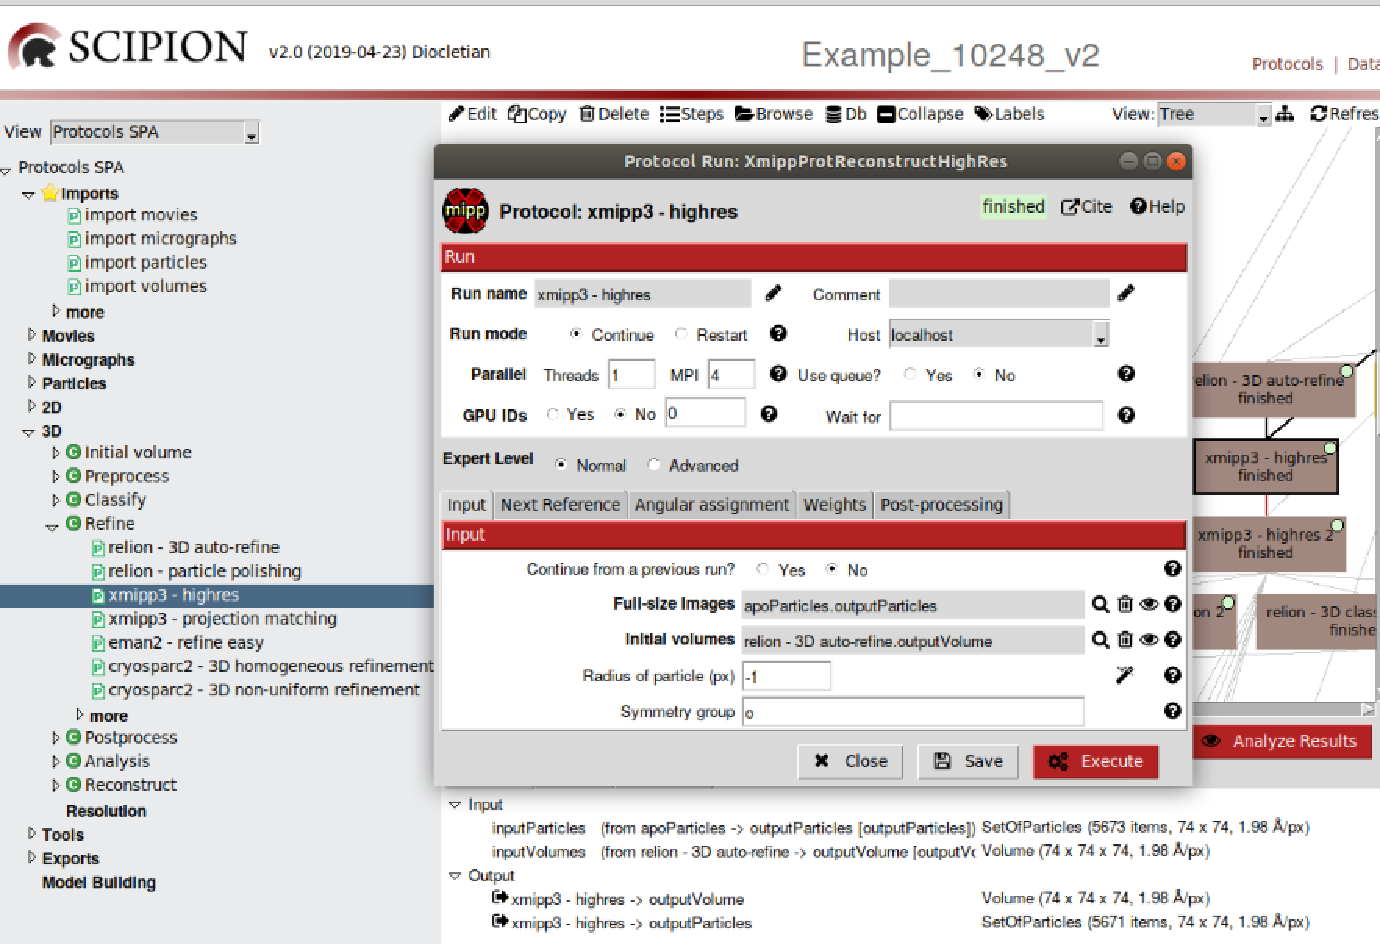
\includegraphics[width=0.95\textwidth]
  {{images/xmipp_highres_1.pdf}}
  \caption{Filling in the params of the protocol \scommand{xmipp3-highres}.}
  \label{fig:xmipp_highres_1}
  \end{figure}

This protocol also generates one map as output with the initial size and sampling rate. Press \scommand{Analyze Results} to check the results of the iteration 1. Particles and map can also visualized. 2 particles have been rejected.\\

The second time that we execute the protocol \scommand{xmipp3-highres} we select the map obtained in the previous step and the same set of particles as input. In the tap \ttt{Angular assignment} we replace \ttt{Global} by \ttt{Local} in the \ttt{Image alignment} param. The rest of the params remain unchanged since we have selected \ttt{Yes} in the param \ttt{Continue from a previous run?} of tap \ttt{Input}. In this case, another map has been generated as output with the same size and sampling rate. 6 particles have been discarded this time.\\

To continue with the refinement process and to obtain a better resolution, we are to start executing three times the same algorithm of $Relion$ \ttt{3D classification} that we have implemented in the protocol \scommand{relion-3D classification} (\ffigure{fig:relion_3Dclassification}). In the tap \ttt{Input} we include the particles derived from executing the previous protocol \scommand{xmipp3-highres}. The map derived from this protocol will be the \ttt{Input volume(s)} in the tap \ttt{Reference 3D map}. The optimization params appear in the tap \ttt{Optimization}: 3 \ttt{Number of classes} and 25 \ttt{Number of iterations}. As \ttt{Regularisation parameter T} values 3-4 are common for \ttt{3D} classificacion.

\begin{figure}[H]
  \centering
  \captionsetup{width=.8\linewidth} 
  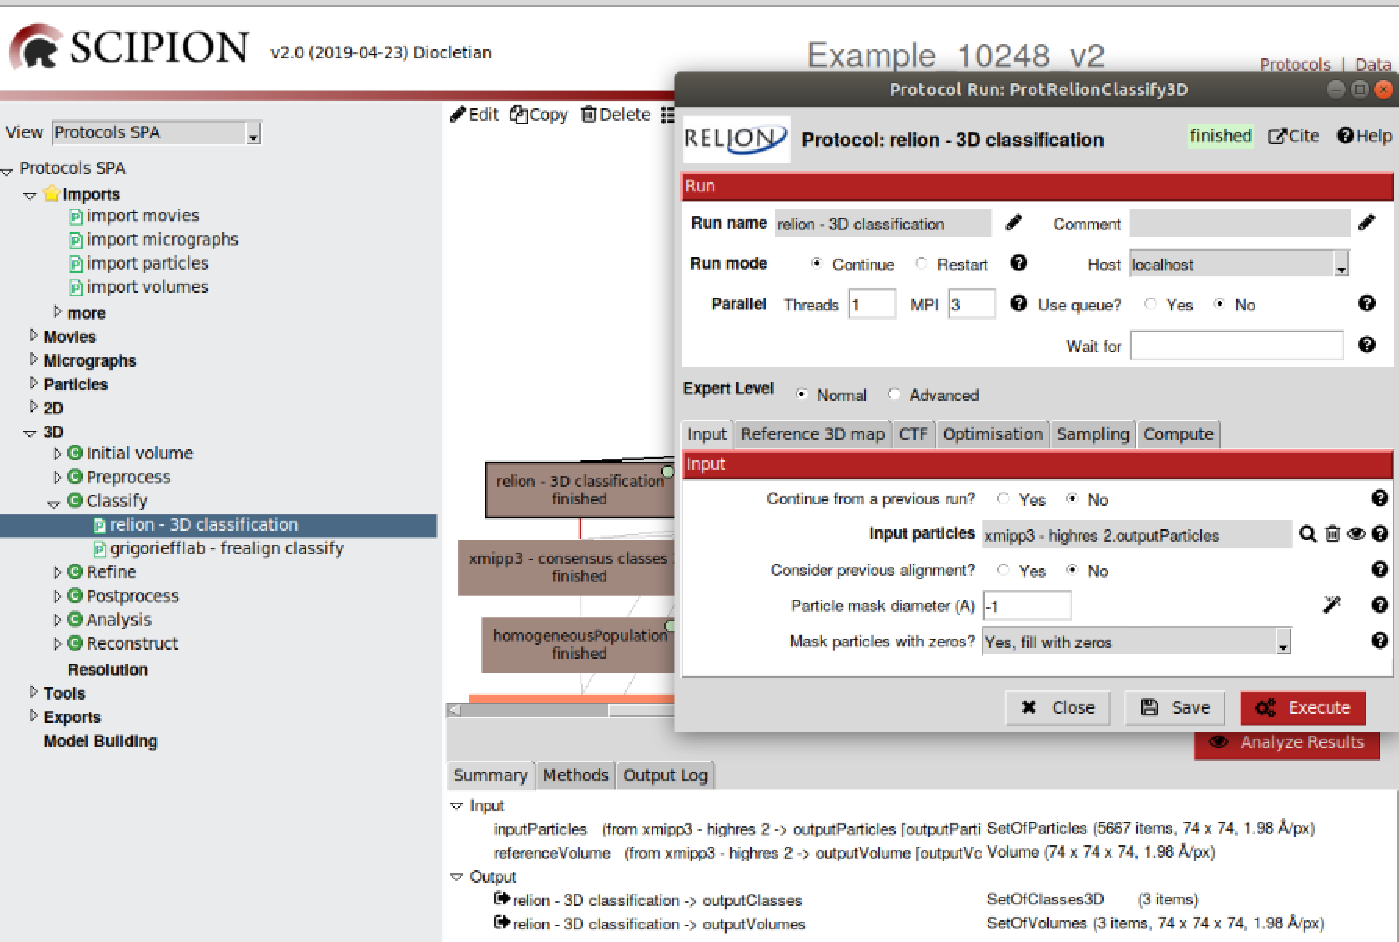
\includegraphics[width=0.95\textwidth]
  {{images/relion_3Dclassification.pdf}}
  \caption{Completing the params of the protocol \scommand{relion-3D classification}.}
  \label{fig:relion_3Dclassification}
  \end{figure}
  
The output of these three protocols are 3 maps 
       

\section{3D refinement}


% \section{A Note on Software Installation}
  All the protocols shown in this document are available in the stable \scipion release \ttt{2.0.0} (code name \textit{Diocletian}). This is a major release in which protocols are published as ``plugins''. Required plugins for each protocol are indicated in respective Appendices. Follow the instructions to install each plugin (\url{https://github.com/scipion-em/}).
  %All the protocols shown in this document will be available in the next stable \scipion release (code name \textit{Diocletian}). This will be a major release in which protocols will be published as ``plugins''. In the meantime, if you want to use the model building protocols you may clone \scipion repository (install git if not present in your system):

  %\begin{verbatim}
   %git clone https://github.com/mmmtnez/scipion.git
   %cd scipion
   %git branch mm_modeling_new
  %\end{verbatim}

  In addition to the standard \scipion and \ttt{scipion plugins} installation, you need to install the following packages:
  
  \begin{itemize}
   \item\textbf{CCP4} (v. 7.0.056 or higher): Connect to \url{http://www.ccp4.ac.uk/download/#os=linux} and follow instructions.
   \item\textbf{Phenix}: Connect to \url{https://www.phenix-online.org/download/} and follow instructions. Protocols have been tested for versions
   1.13-2998 and 1.16-3549.
   \item\textbf{Clustal Omega}: \ttt{sudo apt-get install clustalo} (in ubuntu).
   \item\textbf{MUSCLE}: \ttt{sudo apt-get install muscle} (in ubuntu).
  \end{itemize}

  
  Finally, (1) edit the file \ttt{~/.config/scipion/scipion.conf} and set the right values for the variables \ttt{CCP4\_HOME} and \ttt{PHENIX\_HOME}, and (2) execute \ttt{scipion config --update}

% \section{TODO}

List of protocols in the process to be incorporated:

\begin{itemize}
 \item \textbf{map\_to\_model:} (phenix) \iii{de novo} model building.
 \item \textbf{buccaneer:} (ccp4) \iii{de novo} model building.
\end{itemize}


\bibliographystyle{elsart-harv}
\bibliography{../tutorial_common/em}




%\marginnote{swissmodel}[1cm]
%When predicting by homology a structure is constructed by aligning a target protein sequence with known template structures. The protein sequence can be obtained from many sources, for example NCBI or UniProt. The quality of a structure depends upon the similarity between the target sequence and the database sharing highest similarity is aligned. 

%Esto es otro parrafo


\end{document}

% NOTES
% to be implemented map2model (phenix)
%       chimera (see building parts of a protein without using a template)
